\documentclass[a4paper,12pt, headsepline, ngerman]{scrartcl}

%%%%%%%%%%%%%%%%%%%%%%% PACKAGES %%%%%%%%%%%%%%%%%%%%%%%%%%%%%%%%%%%%%%%%%%%%%%%%
\usepackage{scrlayer-scrpage}
\usepackage[nodisplayskipstretch]{setspace}     %vspace before/after math mode
\usepackage{geometry}
\usepackage{listings}                           %\lstinline[language=C]!while{$a || $b}!
\usepackage{babel}				                %Silbentrennung mit ngerman
\usepackage{booktabs} 			                % For prettier tables
\usepackage{mathtools}  		                %Mathe-Paket
\usepackage{color}				                %\textcolor{blue}{text...}
\usepackage[dvipsnames]{xcolor}                 %Mehr Auswahl bei Farben
\usepackage[T1]{fontenc}		                %Umlaute
\usepackage[utf8]{inputenc}
\usepackage{wrapfig}
\usepackage{caption}
\usepackage{ulem}                               %Durchstreichen von Wörtern mit \sout{text}
\usepackage{enumitem}				            %Aufzählungen [label=\alph*)]
\usepackage{tcolorbox} 				            %Merkboxen
\usepackage{marvosym}                           %\Lightning
\usepackage{multirow}
\usepackage[hidelinks]{hyperref}			                %Hyperlinks setzen
\usepackage[answerdelayed]{exercise}	        %Nach hyperref einbinden!
%%%%%%%%%%%%%% FARBEN %%%%%%%%%%%%%%%%%%%%%%%%%%%%%%%%%%%%%%%%%%%%%%%%%%%%%%%%%%%%%%
\definecolor{codegreen}{rgb}{0,0.6,0}
\definecolor{codegray}{rgb}{0.5,0.5,0.5}
\definecolor{codepurple}{rgb}{0.58,0,0.82}
\definecolor{backcolour}{rgb}{0.95,0.95,0.92}
\definecolor{basiccolour}{rgb}{0.9,0,0.6}
\definecolor{tcback}{rgb}{.95,.95,.95}          %tcolorbox Hintergrund
\definecolor{tcframe}{rgb}{.89,.15,.21}         %tcolorbox Umrandung
%%%%%%%%%%%%%%% KONFIGURATION VON PACKAGES %%%%%%%%%%%%%%%%%%%%%%%%%%%%%%%%%%%%%%%%%%%%
\geometry{a4paper, portrait, left=1.5cm, right=2cm, top=1cm, bottom=2cm, headsep=0.2cm, includehead, head=27.30193pt}
\setlist[enumerate]{nosep, topsep=0pt}	        %Kleinere Abstände bei Aufzählungen
\setlist[itemize]{noitemsep, topsep=0pt}
\lstdefinestyle{mystyle}{
	language=SQL,
	backgroundcolor=\color{backcolour},
	commentstyle=\color{codegreen},
	keywordstyle=\color{magenta},
	numberstyle=\tiny\color{codegray},
	stringstyle=\color{codepurple},
	basicstyle=\color{basiccolour}\ttfamily,
	breakatwhitespace=false,
	breaklines=false,
	captionpos=b,
	keepspaces=false,
	extendedchars=true,
	numbers=left,
	numbersep=5pt,
	showspaces=false,
	showstringspaces=false,
	showtabs=false,
	tabsize=2,
	columns=fullflexible %erzeugt keine komischen Leerzeichen mehr, die man erst beim Kopieren sieht
}
\lstset{style=mystyle}
\lstset{literate=%
	{Ö}{{\"O}}1
	{Ä}{{\"A}}1
	{Ü}{{\"U}}1
	{ß}{{\ss}}1
	{ü}{{\"u}}1
	{ä}{{\"a}}1
	{ö}{{\"o}}1
	{~}{{\textasciitilde}}1
}
\setkomafont{headsepline}{\color{black}}
%Exercise-Paket Umbenennungen
\renewcommand{\listexercisename}{Liste der Aufgaben}%
\renewcommand{\ExerciseName}{Aufgabe}%
\renewcommand{\AnswerName}{L{\"o}sung zu Aufgabe}%
\renewcommand{\ExerciseListName}{Aufg.}%
\renewcommand{\AnswerListName}{L{\"o}sung}%
\renewcommand{\ExePartName}{Teil}%
\renewcommand{\ArticleOf}{von\ }%
\renewcommand{\ExerciseHeader}{%
	\textbf{\large\ExerciseHeaderDifficulty\ExerciseName\ %
	\ExerciseHeaderNB\normalsize\ExerciseHeaderTitle\ExerciseHeaderOrigin}\medskip}
\renewcommand{\AnswerHeader}{
	\medskip\textbf{L{\"o}sung zu \ExerciseName\ \ExerciseHeaderNB}\smallskip}
%tcolorbox Konfiguration
\tcbset{
%	frame code={}
%	center title,
%	left=0pt,
%	right=0pt,
%	top=0pt,
%	bottom=0pt,
	fonttitle=\large\bfseries,
	colback=tcback,
	colframe=tcframe,
%	width=\dimexpr\textwidth\relax,
%	enlarge left by=0mm,
%	boxsep=5pt,
%	arc=0pt,outer arc=0pt,
}
%%%%%%%%%%%%%%%%%%%%%% STYLE %%%%%%%%%%%%%%%%%%%%%%%%%%%%%%%%%%%
\pagestyle{headings} %KOMA-Script mit Kopf-Fuß-Zeilen
\raggedbottom
\raggedright
\onehalfspacing


\begin{document}
	\setlength\parindent{0pt} %keine Einrückungen beim Start eines Paragraphen

	%Header
	\lohead{Datenbanken}
	%\cohead{} %im Arbeitsblatt
	\rohead{}
	\cofoot[\pagemark]{\pagemark}
	\title{Datenbanken

	Ein Skript für das Berufskolleg}
	\author{Hermann Maier}
	\maketitle
	\thispagestyle{empty}
	\newpage
	\null\vfill
	\copyright 2023 Maier, Hermann, \href{mailto:maier@privatemail.com}{maier@privatemail.com}

    Aktuelle Version unter \href{https://github.com/hoerm007/DatenbankenSkript_KaufmBK_BW}{https://github.com/hoerm007/DatenbankenSkript\_KaufmBK\_BW}

    \begin{tcolorbox}\raggedright
        Die verwendeten Datenbanken finden sich unter
        {\small\href{https://github.com/hoerm007/DatenbankenSkript\_KaufmBK\_BW/tree/main/Datenbanken}{https://github.com/hoerm007/DatenbankenSkript\_KaufmBK\_BW/tree/main/Datenbanken}}
    \end{tcolorbox}

	Dieses Werk unterliegt der CC BY-NC-SA 4.0 Lizenz \href{https://creativecommons.org/licenses/by-nc-sa/4.0/legalcode.de}{https://creativecommons.org/licenses/by-nc-sa/4.0/legalcode.de}.

	Sie dürfen:
	\begin{itemize}
		\item Teilen — das Material in jedwedem Format oder Medium vervielfältigen und weiterverbreiten
		\item Bearbeiten — das Material remixen, verändern und darauf aufbauen
	\end{itemize}
	Unter folgenden Bedingungen:
	\begin{itemize}
		\item Namensnennung - Sie müssen angemessene Urheber- und Rechteangaben machen , einen Link zur Lizenz beifügen und angeben, ob Änderungen vorgenommen wurden. Diese Angaben dürfen in jeder angemessenen Art und Weise gemacht werden, allerdings nicht so, dass der Eindruck entsteht, der Lizenzgeber unterstütze gerade Sie oder Ihre Nutzung besonders.
		\item Nicht kommerziell - Sie dürfen das Material nicht für kommerzielle Zwecke nutzen.
		\item Weitergabe unter gleichen Bedingungen - Wenn Sie das Material remixen, verändern oder anderweitig direkt darauf aufbauen, dürfen Sie Ihre Beiträge nur unter derselben Lizenz wie das Original verbreiten.
	\end{itemize}
	\newpage
	\tableofcontents
	\thispagestyle{empty}
	\newpage
	\def\pics{./pics}
	\rohead{Entity-Relationship-Modell}
	% !TeX root = ../Skript_DB.tex
\cohead{\Large\textbf{Grundlagen ERM}}
\section[Enity-Relationship-Modell]{Enity-Relationship-Modell}
\subsection[Datenbanken]{Datenbanken - Einführung}
Datenbanken enthalten, wie der Name schon sagt, große Mengen an Daten, z.B. eine Firma, die ihre Kunden mit Anschrift und die zugehörigen Bestellungen speichern muss. Das Verwalten und Durchsuchen von großen Mengen an Daten ist nicht trivial, z.B. würde Excel schnell an seine Grenzen stoßen, wenn z.B. eine Firma ihre Produkte, Kunden, Bestellungen, usw. speichern will. Datenbanken wurden genau zu diesem Zweck, dem Speichern, Durchsuchen und Bearbeiten von großen Mengen an Daten entwickelt.

Die Daten sollen übersichtlich gespeichert werden und so, dass man sie bearbeiten und durchsuchen kann. Dafür benötigt man eine Struktur. Stellen wir uns vor, eine Firma würde alle Daten, also Bestellungen, Kundendaten, Produktbeschreibungen, Preise, Rechnungen, Daten zu Angestellten, usw. einfach ausdrucken und in einen riesigen Container zusammen werfen. Die Daten wären zwar vorhanden, aber sucht man nun nach der Bestellung von John Wick, weil er sich beschwert, einen Toaster statt eines Eierkochers bekommen zu haben, so würde dies exorbitant viel Zeit in Anspruch nehmen. Würde man jedoch alle Bestellungen zusammen in einem Ordner sammeln, wäre die Suche deutlich einfacher. Die Daten sind dann strukturiert und damit übersichtlicher und einfacher zu durchsuchen bzw. zu bearbeiten. Etwas Ähnliches macht man auch mit den Daten in einer Datenbank. Sehr häufig wird das Enity-Relationship-Modell (ERM) verwendet, um die Daten zu strukturieren.
\subsection[Grundlagen]{Enity-Relationship-Modell}
Das Enity-Relationship-Modell (ERM) dient dazu die Struktur von Daten darzustellen, z.B., dass ein Kunde über einen Namen, Vornamen und eine Adresse verfügt. Wie genau ein bestimmter Kunde heißt oder wo er wohnt spielt für das ERM keine Rolle. Das ERM stellt also nur die Struktur dar, nicht aber den Inhalt. Dazu wird eine Grafik, das ER-Diagramm angefertigt sowie eine Beschreibung der Elemente dieser Grafik. In unseren Beispielen werden die Elemente selbsterklärend sein und wir werden uns die Beschreibung sparen (Im obigen Beispiel ist klar, was Name, Vorname und Adresse des Kunden sind. Es ist keine zusätzliche Beschreibung notwendig).

Für die grafische Darstellungen werden wir die \texttt{Chen-Notation} verwenden. Die wesentlichen Elemente eines ERMs sind:
\begin{tcolorbox}[title=Entitätstypen und Entitäten]
	Darstellung eines meistens in der Realität vorhandenen Objekts auf der Datenbank, z.B. Kunden, Schüler oder Rechnungen. Der Entitätstyp ist die abstrakte Darstellung, z.B. Schüler, während eine Entität eine konkrete Ausprägung, also ein Beispiel ist. So wäre der Schüler Momen Subotic eine Entität in der Datenbank des Entitätstyps Schüler.

	Weitere Beispiele für Entitäten sind:
	\begin{itemize}
		\item Individuen: Person Heinrich Müller, Firma GehtganzGut, Kunde Maria Meyer
		\item Konkreter Gegenstand: Raum A-308, Abteilung Lohn\&Gehalt, Wohnort Berlin
		\item Ereignis: Buchung, Mahnung, Vermietung
		\item Abstraktes: Unterricht, Klasse, Zahlungsart, Tagesplan
	\end{itemize}
	Eine Entität ist immer Mitglied einer Gruppe, auch Entitätstyp genannt. Diese kategorisiert also Entitäten mit gleichen Eigenschaften. So sind z.B. die Schülerin Christine Adler und der Schüler Christopher Jäger konkrete individuell identifizierbare Objekte, zu denen Informationen gespeichert werden. Da sie aber die gleichen Eigenschaften haben, gehören sie zum Entitätstyp Schüler. Welche Objekte so wichtig sind, dass sie als Entitätstyp in das Datenbankmodell aufgenommen werden sollen, muss sich an den funktionellen und informatorischen Zusammenhängen der zu speichernden Daten orientieren.

	Der Entitätstyp, also die Menge der Entitäten, wird in der grafischen Darstellung des ER-Modells, dem ER-Diagramm, als Rechteck dargestellt und die Bezeichnung eines Entitätstyps ist immer ein Substantiv, das wir im Plural verwenden.
\end{tcolorbox}
\begin{tcolorbox}[title=Beziehungen]
	Verknüpfungen von Entitäten, z.B. ist eine Rechnung immer einem bestimmten Kunden zugeordnet. Oft kann ein Entitätstyp Beziehungen zu vielen anderen Entitätstypen haben. So könnte die Rechnung nicht nur mit einem Kunden, sondern auch mit dem Entitätstyp Produkt verknüpft sein, der die bestellten Waren angibt.

	Durch Beziehungen werden die Wechselwirkungen oder Abhängigkeiten von Entitäten ausgedrückt. Beziehungen können ebenfalls Attribute (Eigenschaften) besitzen. Ein Beziehungstyp ist, analog zum Entitätstyp, die Abstraktion gleichartiger Beziehungen. Die Beziehung wird dabei meist durch Verben beschrieben und soll in Beziehungsrichtung einen vollständigen Satz ergeben.

	Beispiele für Beziehungen:
	\begin{itemize}
		\item Kind gehört zu Eltern
		\item Team verfügt über Betreuer
		\item Team besteht aus Teammitglied
	\end{itemize}
	Der Beziehungstyp wird grafisch durch eine Raute dargestellt, die durch zwei Kanten mit den Entitätstypen verbunden ist. In der Raute steht der Name des Beziehungstyps.
\end{tcolorbox}
\begin{tcolorbox}[title=Attribute]
	Attribute, auch als Eigenschaft oder Merkmal bezeichnet, beschreiben die Entitäten näher. Alle Entitäten eines Entitätstyps besitzen dieselben Attribute, jedoch sind die Attributswerte unterschiedlich. Attribute bzw. die Werte der Attribute charakterisieren also einen Entitätstyp bzw. eine Entität oder einen Beziehungstyp bzw. eine Beziehung.

	Beispiele für Attribute:
	\begin{itemize}
		\item Name, Vorname oder Adresse einer Person
		\item Betrag einer Rechnung oder Bestellung
		\item Klassengröße oder Klassenzimmer einer Klasse
	\end{itemize}
	In der grafischen Darstellung werden Attribute als Ellipsen oder Kreise dargestellt. Diese sind über ungerichtete Kanten mit dem Entitätstyp verbunden.
\end{tcolorbox}
\begin{minipage}{\textwidth}
	\begin{minipage}{0.33\textwidth}
		\centering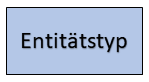
\includegraphics[width=4cm]{\pics/ERMEntity.png}

		Grafische Darstellung eines Entitätstyps.
	\end{minipage}
	\begin{minipage}{0.33\textwidth}
		\centering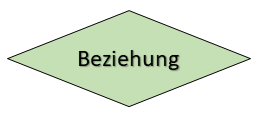
\includegraphics[width=4cm]{\pics/ERMRelationship.png}

		Grafische Darstellung einer Beziehung.
	\end{minipage}
	\begin{minipage}{0.33\textwidth}
		\centering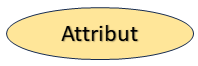
\includegraphics[width=4cm]{\pics/ERMAttribute.png}

		Grafische Darstellung eines Attributs.
	\end{minipage}
\end{minipage}
\begin{Exercise}[title={Beantworte folgende Fragen.}, label=ERMFragen1]
	\begin{enumerate}
		\item Worin liegt der Unterschied zwischen Entitäten und Entitätstypen?
		\item Worin liegt der Unterschied zwischen Attributen und Attributswerten?
	\end{enumerate}
\end{Exercise}
%%%%%%%%%%%%%%%%%%%%%%%%%%%%%%%%%%%%%%%%%
\begin{Answer}[ref=ERMFragen1]
	\begin{enumerate}
		\item Worin liegt der Unterschied zwischen Entitäten und Entitätstypen?

		Ein Entitätstyp ist der abstrakte Übergriff, z.B. Schüler, während eine Entität ein konkretes Beispiel ist, z.B. der Schüler Noah Schimek ist eine Entität vom Entitätstyp Schüler.
		\item Worin liegt der Unterschied zwischen Attributen und Attributswerten?

		Auch hier ist das Attribut die abstrakte Eigenschaft, z.B. hat der Entitätstyp Schüler ein Attribut Namen. Den Wert eines Attributs erhält man, wenn man eine bestimmte Entität betrachtet, z.B. hat das Attribut Namen beim obigen Schüler den Wert Noah Schimek.
	\end{enumerate}
\end{Answer}
\begin{Exercise}[title={Erstelle jeweils ein ERM}, label=ERMErstellen1]
	\begin{enumerate}
		\item Ein Fahrradverleih am Bodensee verleiht Damen-, Herren- und Kinderfahrräder. Dabei wird für jedes Fahrrad ein eigener Mietvertrag abgeschlossen. Eine Person kann mehrere Fahrräder mieten. Der Fahrradverleih möchte eine Datenbank aufbauen. Helfen Sie dabei.
		\item Ein befreundeter Autohändler bittet uns beim Aufbau einer Kundendatenbank zu helfen. Zuerst soll diese in einem ERM modelliert werden. Darin erscheinen sollen Kunde, Auto, Karosserietyp und Reifen. Ein Auto gehört dabei zu einem Kunden, ein Kunde kann aber mehrere Autos haben.
		\item Ein DVD-Verleiher betreibt mehrere Filialen (id, strasse, plz), wo es jeweils mehrere Medien (DVDs, BluRays, Spiele) zu leihen gibt. Jeder Kunde kann nur einer Filiale zugeordnet sein. Jeder Kunde kann mehrere Medien ausleihen. Ein Mitarbeiter kann nur in einer Filiale arbeiten.
	\end{enumerate}
\end{Exercise}
%%%%%%%%%%%%%%%%%%%%%%%%%%%%%%%%%%%%%%%%%
\begin{Answer}[ref=ERMErstellen1]
	Anmerkung: Die ERMs sind nur Lösungsvorschläge. Man kann auch zusätzliche Attribute hinzufügen. Zudem sind die ERMs nicht vollständig, wir werden später noch neue Begriffe kennen lernen, die hier noch fehlen.
	\begin{enumerate}
		\item Ein Fahrradverleih am Bodensee verleiht Damen-, Herren- und Kinderfahrräder. Dabei wird für jedes Fahrrad ein eigener Mietvertrag abgeschlossen. Eine Person kann mehrere Fahrräder mieten. Der Fahrradverleih möchte eine Datenbank aufbauen. Helfen Sie dabei.

		\begin{minipage}{0.8\textwidth}
			\centering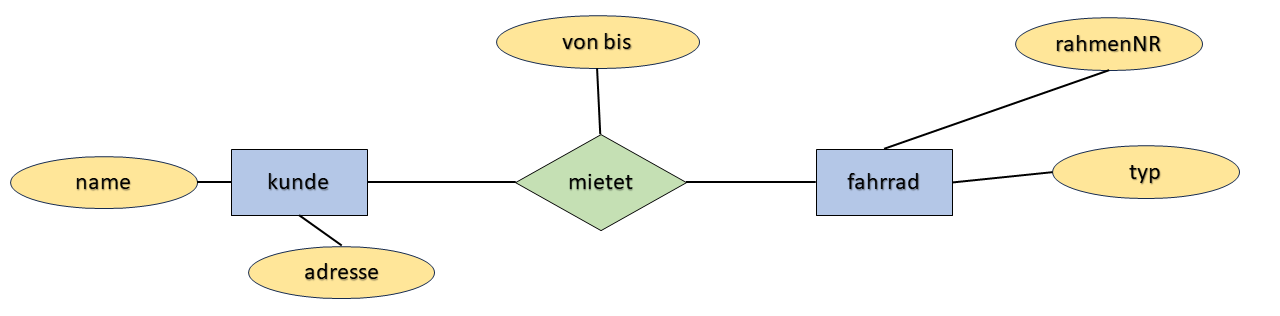
\includegraphics[width=\textwidth]{\pics/ERMFahrrad.png}
		\end{minipage}

		\item Ein befreundeter Autohändler bittet uns beim Aufbau einer Kundendatenbank zu helfen. Zuerst soll diese in einem ERM modelliert werden. Darin erscheinen sollen Kunde, Auto, Karosserietyp und Reifen. Ein Auto gehört dabei zu einem Kunden, ein Kunde kann aber mehrere Autos haben.

		\begin{minipage}{0.8\textwidth}
			\centering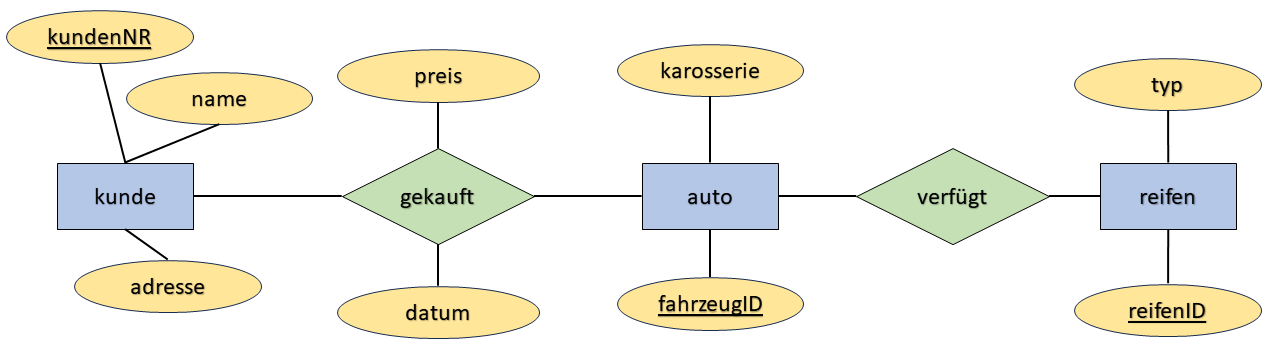
\includegraphics[width=\textwidth]{\pics/ERMAuto.png}
		\end{minipage}

		\item Ein DVD-Verleiher betreibt mehrere Filialen (id, strasse, plz), wo es jeweils mehrere Medien (DVDs, BluRays, Spiele) zu leihen gibt. Jeder Kunde kann nur einer Filiale zugeordnet sein. Jeder Kunde kann mehrere Medien ausleihen. Ein Mitarbeiter kann nur in einer Filiale arbeiten.

		\begin{minipage}{0.8\textwidth}
			\centering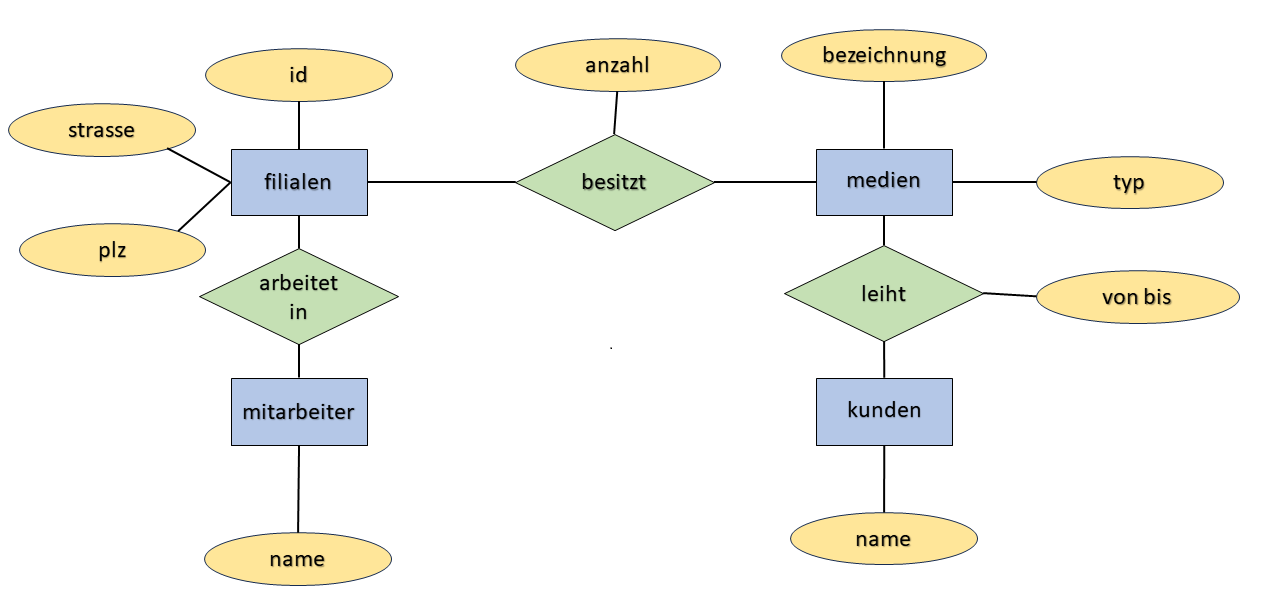
\includegraphics[width=\textwidth]{\pics/ERMDVDs.png}
		\end{minipage}
	\end{enumerate}
\end{Answer}

\subsection{Primärschlüssel und Kardinalitäten}
Der Primärschlüssel löst das Problem der Eindeutigkeit. Jede Entität, die auf der Datenbank gespeichert wird, muss eindeutig identifizierbar sein. Speichert z.B. eine Firma eine Entität  vom Typ Kunden, so muss jeder Kunde eindeutig identifizierbar sein. Würde man als Attribute nur den Namen und Vornamen anhängen, so könnte man Diego Maradonna aus Bremen nicht von Diego Maradonna aus Stuttgart unterscheiden. Man kann natürlich einfach zusätzliche Attribute hinzufügen, wie z.B. das Geburtsdatum oder die Adresse, bis man sich sicher ist, dass es nicht zu Verwechslungen kommen kann, aber es gibt einen eleganteren Weg. Im Normalfall hängt man eine Nummer an (z.B. die Kundennummer), die für jede Entität eine andere sein muss. So kann man jede Entität eindeutig an Hand der Nummer identifizieren. Diego mit der Kundennummer 44445 ist dann eine andere Person als Diego mit der Kundennummer 85417. Diese Nummer bezeichnet man Primärschlüssel.
\begin{tcolorbox}[title=Primärschlüssel]
	Attribut, das eine Entität eindeutig identifizierbar macht. Im Normalfall eine laufende Nummer, d.h. bei jeder neu hinzukommenden Entität wird die Nummer einfach um eins größer gemacht. Der Primärschlüssel wird im ERM durch Unterstreichen kenntlich gemacht.
\end{tcolorbox}
\begin{tcolorbox}[title=Fremdschlüssel]
	Wird der Primärschlüssel eines Entitätstyps an einen anderen Entitätstyp als Attribut hinzugefügt, so bezeichnet man dieses Attribut als Fremdschlüssel.
\end{tcolorbox}
Die Kardinalität gehört zu Beziehungen und gibt an, wie viele Entitäten jeweils in Beziehung zueinander stehen können. Diesen Angaben schreibt man auf die Kanten zwischen den jeweiligen Entitätstypen und der Beziehung. Man unterscheidet im Wesentlichen folgende Kardinalitäten:

\begin{itemize}
	\item 1:1 Beziehung

	Jede Entität des einen Typs \(E_1\) ist maximal einer Entität des anderen Typs \(E_2\) zugeordnet und umgekehrt, z.B. hat jedes Land genau eine Hauptstadt und jede Hauptstadt liegt in genau einem Land.
	\begin{minipage}{0.8\textwidth}
		\centering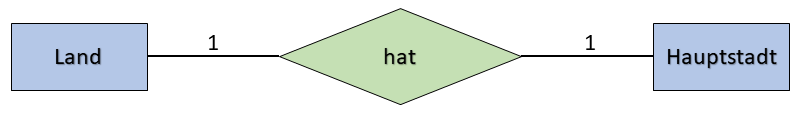
\includegraphics[width=\textwidth]{\pics/ERMBeziehungen11.png}
		Grafische Darstellung einer 1:1 Beziehung.
	\end{minipage}
	\item 1:N Beziehung

	Jeder Entität des einen Typs \(E_1\) sind beliebig viele Entitäten des zweiten Typs \(E_2\) zugeordnet. Umgekehrt sind jedoch jeder Entität vom Typ \(E_2\) maximal eine Entität vom Typ \(E_1\) zugeordnet, z.B. gehen mehrere Schüler in eine Klasse, umgekehrt geht aber ein einzelner Schüler in genau eine Klasse.

	\begin{minipage}{0.8\textwidth}
		\centering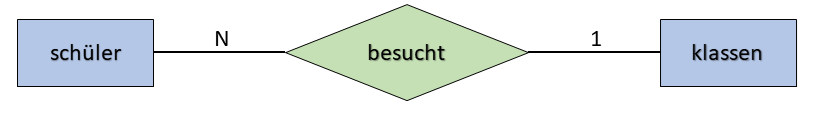
\includegraphics[width=\textwidth]{\pics/ERMBeziehungen1N.png}

		Grafische Darstellung einer 1:N Beziehung.
	\end{minipage}
	\item N:M Beziehung

	Jeder Entität des einen Typs \(E_1\) sind beliebig viele Entitäten des zweiten Typs \(E_2\) zugeordnet und umgekehrt, z.B. kann ein Mitarbeiter an mehreren Projekten gleichzeitig arbeiten und umgekehrt können an einem Projekt mehrere Mitarbeiter gleichzeitig arbeiten.

	\begin{minipage}{0.8\textwidth}
		\centering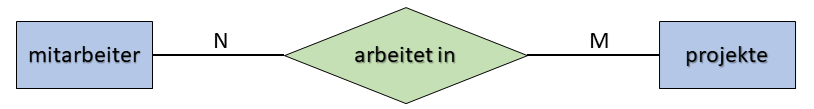
\includegraphics[width=\textwidth]{\pics/ERMBeziehungenNM.png}

		Grafische Darstellung einer N:M Beziehung.
	\end{minipage}
\end{itemize}

\subsection{Beispiel eines ERMs einer Firma}
Die Kunden einer Firma können Bestellungen aufgeben, die ein oder mehrere Artikel enthalten. Zu jeder Bestellung erhält der Kunde eine Rechnung. Für die Firma wichtig sind Name und Adresse der Kunden, das Datum der Bestellung, welche Artikel enthalten sind und wie teuer diese sind sowie der Betrag und das Fälligkeitsdatum der Rechnung:

\begin{minipage}{\textwidth}
	\centering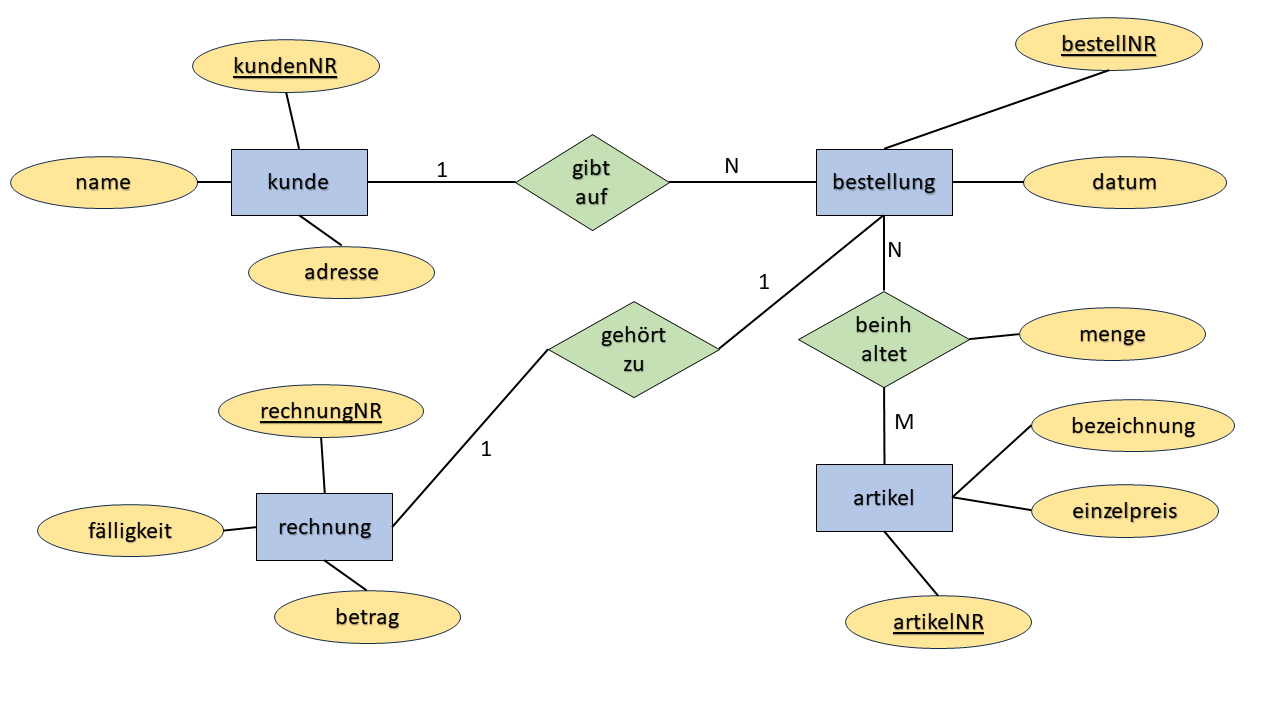
\includegraphics[width=\textwidth]{\pics/ERMFirmaEinfach.png}
\end{minipage}

Beispiel für ein ERM. Die Primärschlüssel sind jeweils unterstrichen. Die Kardinalitäten der Beziehungen ergeben sich aus folgenden Überlegungen:
\begin{itemize}
	\item Kunden zu Bestellungen eine 1:N Beziehung. Ein Kunde kann mehrere Bestellungen aufgeben, aber jede Bestellung ist genau einem Kunden zugeordnet.
	\item Rechnungen zu Bestellungen eine 1:1 Beziehung. Hinter jeder Rechnung verbirgt sich genau eine Bestellung und zu jeder Bestellung wird genau eine Rechnung erstellt.
	\item Bestellungen zu Artikel eine N:M Beziehung. In jeder Bestellung können mehrere (M verschiedene) Artikel vorkommen und umgekehrt kann ein Artikel in verschiedenen Bestellungen (N verschiedene) vorkommen.
\end{itemize}
\begin{Exercise}[title=Vervollständige die ERMs aus Aufgabe \ref{ERMErstellen1}. Jeder Entitätstyp muss einen Primärschlüssel haben und ergänze die Kardinalitäten., label=ERMErstellen2]
	\phantom{ }
\end{Exercise}%
%%%%%%%%%%%%%%%%%%%%%%%%%%%%%%%%%%%%%%%%%%
\begin{Answer}[ref=ERMErstellen2]
	\begin{enumerate}
		\item Ein Fahrradverleih am Bodensee verleiht Damen-, Herren- und Kinderfahrräder. Dabei wird für jedes Fahrrad ein eigener Mietvertrag abgeschlossen. Eine Person kann mehrere Fahrräder mieten. Der Fahrradverleih möchte eine Datenbank aufbauen. Helfen Sie dabei.

		\begin{minipage}{0.8\textwidth}
			\centering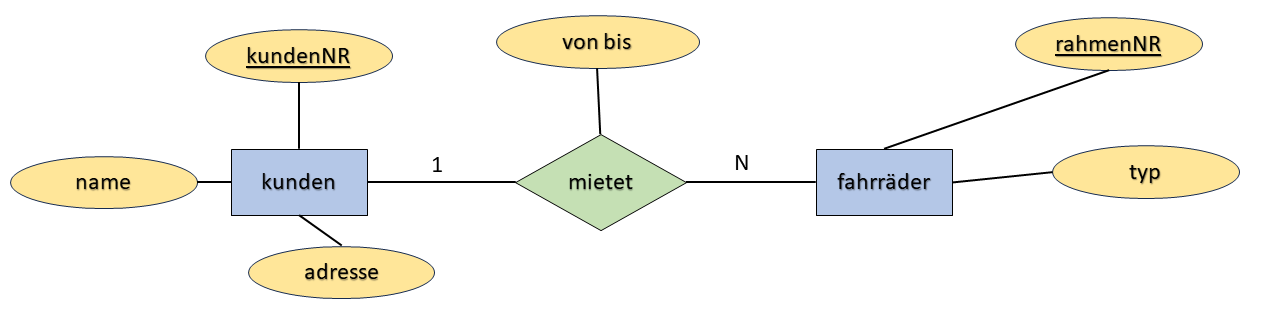
\includegraphics[width=\textwidth]{\pics/ERMFahrradvoll.png}
		\end{minipage}
		\item Ein befreundeter Autohändler bittet uns beim Aufbau einer Kundendatenbank zu helfen. Zuerst soll diese in einem ERM modelliert werden. Darin erscheinen sollen Kunde, Auto, Karosserietyp und Reifen. Ein Auto gehört dabei zu einem Kunden, ein Kunde kann aber mehrere Autos haben.

		\begin{minipage}{0.8\textwidth}
			\centering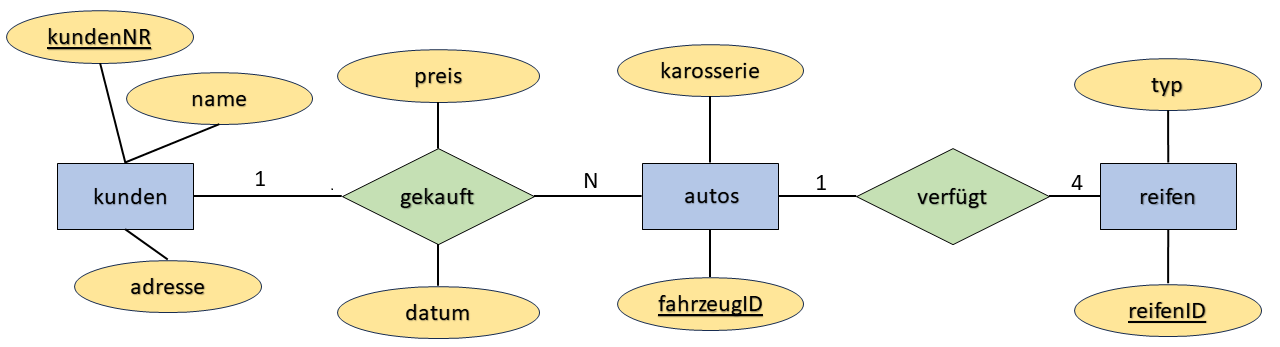
\includegraphics[width=\textwidth]{\pics/ERMAutovoll.png}
		\end{minipage}
		\item Ein DVD-Verleiher betreibt mehrere Filialen (id, strasse, plz), wo es jeweils mehrere Medien (DVDs, BluRays, Spiele) zu leihen gibt. Jeder Kunde kann nur einer Filiale zugeordnet sein. Jeder Kunde kann mehrere Medien ausleihen. Ein Mitarbeiter kann nur in einer Filiale arbeiten.

		\begin{minipage}{0.8\textwidth}
			\centering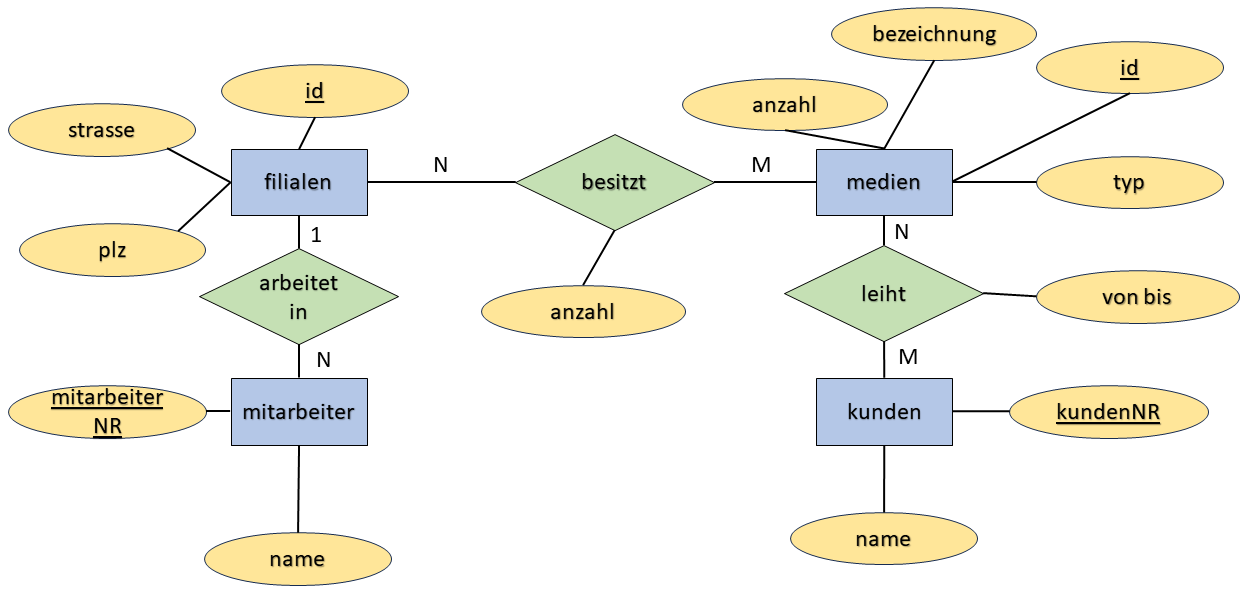
\includegraphics[width=\textwidth]{\pics/ERMDVDsvoll.png}
		\end{minipage}
	\end{enumerate}
\end{Answer}
\newpage
\begin{Exercise}[title=Erstelle ein ERM., label=ERMErstellen3]

	In der Oberstufe eines Gymnasiums wird nicht mehr in Klassen, sondern in Kursen unterrichtet. Sie erhalten von der Schulleitung den Auftrag, eine Kursverwaltung mittels des Entity-Relationship-Modells zu modellieren. Mit Hilfe dieser Kursverwaltung soll festgehalten werden, welche Schüler welche Kurse besuchen. Als Schülerdaten soll neben dem Vornamen und Nachnamen der Schüler auch die individuelle Schülernummer, das Geburtsdatum, Geschlecht sowie die Postadresse festgehalten	werden. Jeder Kurs hat eine eigene Kursnummer. Außerdem sind der Kurstyp (5stündig / 2stündig), das Fach (z.B. D, M, E, …) und die Jahrgangsstufe (K1 oder K2) zu speichern. In dem neuen System sollen auch die Fehlstunden und Kursnoten jedes Schülers dokumentiert werden. Jeder Kurs ist einem Lehrer zugeordnet. Als lehrerspezifische Daten sollen dessen Vor- und Nachname, das Kürzel und seine Fächer (max. 2) mit in das Kursverwaltungsprogramm aufgenommen werden.
\end{Exercise}

\begin{Answer}[ref=ERMErstellen3]

	In der Oberstufe eines Gymnasiums wird nicht mehr in Klassen, sondern in Kursen unterrichtet. Sie erhalten von der Schulleitung den Auftrag, eine Kursverwaltung mittels des Entity-Relationship-Modells zu modellieren. Mit Hilfe dieser Kursverwaltung soll festgehalten werden, welche Schüler welche Kurse besuchen. Als Schülerdaten soll neben dem Vornamen und Nachnamen der Schüler auch die individuelle Schülernummer, das Geburtsdatum, Geschlecht sowie die Postadresse festgehalten werden. Jeder Kurs hat eine eigene Kursnummer. Außerdem sind der Kurstyp (5stündig / 2stündig), das Fach (z.B. D, M, E, …) und die Jahrgangsstufe (K1 oder K2) zu speichern. In dem neuen System sollen auch die Fehlstunden und Kursnoten jedes Schülers dokumentiert werden. Jeder Kurs ist einem Lehrer zugeordnet. Als lehrerspezifische Daten sollen dessen Vor- und Nachname, das Kürzel und seine Fächer (max. 2) mit in das Kursverwaltungsprogramm aufgenommen werden.

	\begin{minipage}{\textwidth}
		\centering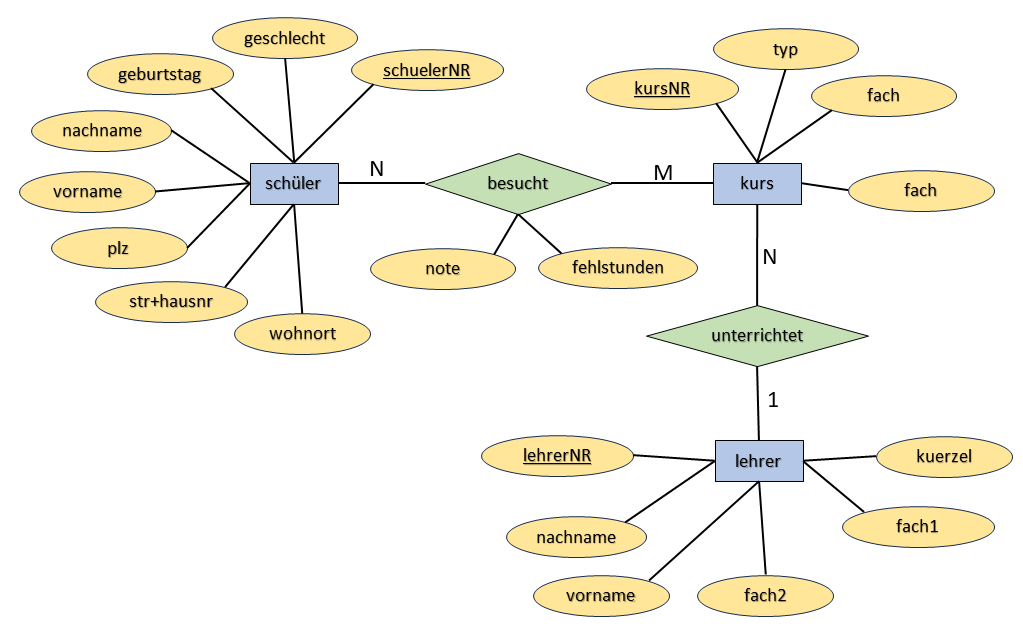
\includegraphics[width=\textwidth]{\pics/ERMOberstufe.png}
	\end{minipage}
\end{Answer}

	\newpage
	\subsection[Darstellung auf der DB]{Darstellung auf der Datenbank}
Einerseits ist die Darstellung eines ERMs auf der Datenbank simpel. Jeder Entitätstyp und jede Beziehung kann als Tabelle dargestellt werden. Andererseits ergeben sich aus der Darstellung bestimmte Regeln zum Erstellen eines guten ERMs, die wir unter dem Kapitel Normalisierung besprechen werden.\\
\begin{tcolorbox}[title=Entitäten/-typen und Beziehungen auf der Datenbank]
	Entitäten bzw. Entitätstypen und Beziehungen werden als Tabellen auf der Datenbank vorgestellt. Eine Tabelle besteht aus einer Überschrift, die den Entitätstyp bzw. die Beziehung angibt, den Spaltenüberschriften, die die Attribute darstellen und den Zeilen mit konkreten Werten. Die Werte einzelner Zellen stehen dabei für die Attributswerte während eine ganze Zeile eine Entität repräsentiert.
\end{tcolorbox}
Beispiel für die Entitätstypen Schüler, Lehrer und Abteilung. Für die Namen auf der Datenbank wird im Skript folgende Notation verwendet: \lstinline!schueler!\\\phantom{ }\\
\begin{tabular}{llll}
	\multicolumn{4}{c}{\lstinline!schueler!}\\
	\hline
	\underline{\lstinline!schuelerNR!}&\lstinline!name!&\lstinline!klasse!&\lstinline!klassenlehrer!\\
	\hline
	15&Waylon Smithers&BK22&Krabappel\\
	24&Moe Szyslak&BK13&Skinner\\
	102&Homer Simpson&BK22&Krabappel\\
	9&Apu Nahasapeemapetilon&WG32&Krabappel\\
	47&Carl Carlson&BK12&Skinner\\
\end{tabular}\\
\begin{tabular}{lll}
	\multicolumn{3}{c}{\lstinline!abteilung!}\\
	\hline
	\underline{\lstinline!abteilungNR!}&\lstinline!bezeichnung!&\lstinline!abteilungsleiter!\\
	\hline
	1&Berufskolleg&Krabappel\\
	2&Wirtschaftsgymnasium&Hoover\\
\end{tabular}\\
\begin{tabular}{lll}
	\multicolumn{3}{c}{\lstinline!lehrer!}\\
	\hline
	\underline{\lstinline!lehrerNR!}&\lstinline!name!&\lstinline!kuerzel!\\
	\hline
	24&Krabappel&KRB\\
	30&Skinner&SKI\\
	31&Hoover&HOO\\
\end{tabular}\\
Wie wir später sehen werden, ist das gewählte ERM noch stark verbesserungsfähig. Vorerst wollen wir aber jeden Lehrer genau einer Abteilung zuordnen. Diese Beziehung kann ebenfalls über eine Tabelle dargestellt werden:\\
\begin{tabular}{lll}
	\multicolumn{3}{c}{\lstinline!abteilung_lehrer!}\\
	\hline
	\underline{\lstinline!lfdNR!}&\lstinline!abteilungNR!&\lstinline!lehrerNR!\\
	\hline
	1&1&24\\
	2&1&30\\
	3&2&31\\
\end{tabular}\\
In der Tabelle \lstinline!abteilung_lehrer! könnte man die \lstinline!lfdNR! als Primärschlüssel auch streichen und stattdessen die \lstinline!abteilungNR! und \lstinline!lehrerNR! zusammen als Primärschlüssel verwenden. Außer dem geringfügig größeren Speicherbedarf spricht aber für unsere Zwecke nichts gegen das Hinzufügen einer laufenden Nummer als Primärschlüssel. Die erste Entität bzw. Zeile sagt nun aus, dass der Abteilung mit der \lstinline!abteilungNR! 1, also dem Berufskolleg, der Lehrer mit der \lstinline!lehrerNR! 24, also Krabappel, angehört. In der zweiten Zeile bzw. Entität steht, dass dem Berufskolleg außerdem auch Skinner angehört. Und die dritte Zeile besagt, dass dem Wirtschaftsgymnasium Hoover angehört.\\
Beachte, dass der Primärschlüssel auch hier unterstrichen ist und aus Gründen der Übersichtlichkeit immer an erster Stelle steht.
\begin{Exercise}[title=Erstelle zu den ERMs aus \ref{ERMErstellen1} passende Tabellen., label=TabelleErstellen1]

\end{Exercise}
%%%%%%%%%%%%%%%%%%%%%%%%%%%%%%%%%%%%%%%%%%
\begin{Answer}[ref=TabelleErstellen1]
	\begin{enumerate}
		\item Ein Fahrradverleih am Bodensee verleiht Damen-, Herren- und Kinderfahrräder. Dabei wird für jedes Fahrrad ein eigener Mietvertrag abgeschlossen. Eine Person kann mehrere Fahrräder mieten. Der Fahrradverleih möchte eine Datenbank aufbauen. Helfen Sie dabei.\\
		\begin{tabular}{lll}
			\multicolumn{3}{c}{\lstinline!kunde!}\\
			\hline
			\underline{\lstinline!kundeNR!}&\lstinline!name!&\lstinline!adresse!\\
			\hline
			15&Fathi Russdi&Rotgasse 12, 55555 Bielefeld\\
		\end{tabular}\\
		\begin{tabular}{ll}
			\multicolumn{2}{c}{\lstinline!fahrrad!}\\
			\hline
			\underline{\lstinline!rahmenNR!}&\lstinline!typ!\\
			\hline
			18498451&Rennrad\\
			89415456&Kinderrad\\
		\end{tabular}\\
		\begin{tabular}{lllll}
			\multicolumn{5}{c}{\lstinline!mietet!}\\
			\hline
			\underline{\lstinline!laufendeNR!}&\lstinline!kundenNR!&\lstinline!rahmenNR!&\lstinline!beginn!&\lstinline!ende!\\
			\hline
			1&15&18498451&01.09.2023&03.09.2023\\
			2&15&89415456&01.09.2023&03.09.2023\\
		\end{tabular}\\
		\item Ein befreundeter Autohändler bittet uns beim Aufbau einer Kundendatenbank zu helfen. Zuerst soll diese in einem ERM modelliert werden. Darin erscheinen sollen Kunde, Auto, Karosserietyp und Reifen. Ein Auto gehört dabei zu einem Kunden, ein Kunde kann aber mehrere Autos haben.\\
		\begin{tabular}{lll}
			\multicolumn{3}{c}{\lstinline!kunde!}\\
			\hline
			\underline{\lstinline!kundeNR!}&\lstinline!name!&\lstinline!adresse!\\
			\hline
			15&Fathi Russdi&Rotgasse 12, 55555 Bielefeld\\
		\end{tabular}\\
		\begin{tabular}{ll}
			\multicolumn{2}{c}{\lstinline!auto!}\\
			\hline
			\underline{\lstinline!fahrzeugID!}&\lstinline!karosserie!\\
			\hline
			189765465451&Kübelwagen\\
		\end{tabular}\\
		\begin{tabular}{ll}
			\multicolumn{2}{c}{\lstinline!reifen!}\\
			\hline
			\underline{\lstinline!reifenID!}&\lstinline!typ!\\
			\hline
			89454115&Winterreifen\\
		\end{tabular}\\
		\begin{tabular}{lll}
			\multicolumn{3}{c}{\lstinline!auto_reifen!}\\
			\hline
			\underline{\lstinline!laufendeNR!}&\lstinline!fahrzeugID!&\lstinline!reifenID!\\
			\hline
			4&189765465451&89454115\\
		\end{tabular}\\
		\begin{tabular}{lllll}
			\multicolumn{5}{c}{\lstinline!auto_kunde!}\\
			\hline
			\underline{\lstinline!laufendeNR!}&\lstinline!fahrzeugID!&\lstinline!kundenNR!&\lstinline!preis!&\lstinline!datum!\\
			\hline
			119&189765465451&15&43000&10.08.2023\\
		\end{tabular}\\
		\item Ein DVD-Verleiher betreibt mehrere Filialen (id, strasse, plz), wo es jeweils mehrere Medien (DVDs, BluRays, Spiele) zu leihen gibt. Jeder Kunde kann nur einer Filiale zugeordnet sein. Jeder Kunde kann mehrere Medien ausleihen. Ein Mitarbeiter kann nur in einer Filiale arbeiten.\\
		\begin{tabular}{lll}
			\multicolumn{3}{c}{\lstinline!filiale!}\\
			\hline
			\underline{\lstinline!filialID!}&\lstinline!strasse!&\lstinline!plz!\\
			\hline
			3&Königsbau 4&70174\\
		\end{tabular}\\
		\begin{tabular}{ll}
			\multicolumn{2}{c}{\lstinline!mitarbeiter!}\\
			\hline
			\underline{\lstinline!mitarbeiterNR!}&\lstinline!name!\\
			\hline
			47&Agent 47\\
		\end{tabular}\\
		\begin{tabular}{llll}
			\multicolumn{4}{c}{\lstinline!medium!}\\
			\hline
			\underline{\lstinline!medienID!}&\lstinline!bezeichnung!&\lstinline!anzahl!&\lstinline!typ!\\
			\hline
			1002&The matrix&5&DVD\\
		\end{tabular}\\
		\begin{tabular}{ll}
			\multicolumn{2}{c}{\lstinline!kunde!}\\
			\hline
			\underline{\lstinline!kundenNR!}&\lstinline!name!\\
			\hline
			50&Lucky Luke\\
		\end{tabular}\\
		\begin{tabular}{lll}
			\multicolumn{3}{c}{\lstinline!filiale_mitarbeiter!}\\
			\hline
			\underline{\lstinline!laufendeNR!}&\lstinline!filialID!&\lstinline!mitarbeiterNR!\\
			\hline
			1&3&47\\
		\end{tabular}\\
		\begin{tabular}{llll}
			\multicolumn{4}{c}{\lstinline!filiale_medium!}\\
			\hline
			\underline{\lstinline!laufendeNR!}&\lstinline!filialID!&\lstinline!medienID!&\lstinline!anzahl!\\
			\hline
			1&3&1002&2\\
		\end{tabular}\\
		\begin{tabular}{lllll}
			\multicolumn{5}{c}{\lstinline!kunde_medium!}\\
			\hline
			\underline{\lstinline!laufendeNR!}&\lstinline!kundenNR!&\lstinline!medienID!&\lstinline!beginn!&\lstinline!beginn!\\
			\hline
			99&50&1002&01.01.2023&14.01.2023\\
		\end{tabular}\\
	\end{enumerate}
\end{Answer}
	\newpage
	% !TeX root = ../Skript_DB.tex
\cohead{\Large\textbf{Anomalien}}
\subsection[Anomalien]{Anomalien}\label{Anomalien}
Von Anomalien spricht man, wenn die Daten auf der Datenbank inkonsistent sind, also fehlerhaft. Wir unterscheiden folgende Anomalien:

\begin{tcolorbox}[title=Anomalien]
	\begin{enumerate}
		\item \textbf{Änderungs-Anomalien}: Diese können auftreten, wenn Attributswerte an mehreren Stellen geändert werden sollen, jedoch nicht alle Stellen geändert werden.
		\item \textbf{Einfüge-Anomalien}: Diese können auftreten, wenn das Einfügen eines Attributswertes zum zwingenden Einfügen weiterer Attributswerte führt.
		\item \textbf{Lösch-Anomalien}: Diese können auftreten, wenn das Löschen einer Entität das ungewollte Löschen wichtiger Infos (Attributswerte) mit sich bringt.
	\end{enumerate}
\end{tcolorbox}
Zudem entspricht es dem Best Practice Redundanzen (das Speichern der gleichen Information an mehreren Stellen in der Datenbank) zu vermeiden. Betrachten wir folgendes Beispiel:

Unsere Schüler engagieren sich in unterschiedlichen Schulprojekten. Der Verbindungslehrer Herr KeinDBProfi hat zu Verwaltungszwecken folgende Tabelle angelegt:
\begin{tabular}{llllllll}
	\multicolumn{8}{c}{\lstinline!projektinfos!}\\
	\hline
	\underline{\lstinline!schNR!}&\lstinline!name!&\lstinline!vorname!&\lstinline!klasse!&\lstinline!klassenbez!&\lstinline!projektNR!&\lstinline!probez!&\lstinline!prostd!\\
	\hline
	1 &
	Müller &
	Marius &
	BK22 &
	Kaufm. BK2&
	1 &
	Homepage &
	30 \\
	2 &
	Kryof  &
	Yuri &
	BK14 &
	Kaufm. BK1&
	2 &
	Foyergestaltung &
	25 \\
	3 &
	Abadi &
	Ali &
	BK14 &
	Kaufm. BK1&
	1,2 &
	Homepage,&
	10,\\
	&&&&&&Foyergestaltung&15\\
	4 &
	Sanbei &
	Sarah &
	BK22 &
	Kaufm. BK2 &
	1,3 &
	Homepage,&
	15,  \\
	&&&&&&Schulfest&35\\
\end{tabular}

Nun will man folgende Änderungen vornehmen:
\begin{enumerate}
	\item \textcolor{red}{Da es sich um die ÜFA-Homepage handelt, soll die Projekt-Bezeichnung entsprechend geändert werden.}
	\item \textcolor{blue}{Das neue Projekt \texttt{Abschlussfeier} soll in die Tabelle aufgenommen werden.}
	\item \textcolor{ForestGreen}{Die Schüler der BK22 machen ihren Abschluss und verlassen die Schule}
\end{enumerate}
Die geänderte Tabelle sieht nun wie folgt aus:
\begin{tabular}{llllllll}
	\multicolumn{8}{c}{\lstinline!projektinfos!}\\
	\hline
	\underline{\lstinline!schNR!}&\lstinline!name!&\lstinline!vorname!&\lstinline!klasse!&\lstinline!klassenbez!&\lstinline!projektNR!&\lstinline!probez!&\lstinline!prostd!\\
	\hline
	\textcolor{ForestGreen}{\sout{1}} &
	\textcolor{ForestGreen}{\sout{Müller}} &
	\textcolor{ForestGreen}{\sout{Marius}} &
	\textcolor{ForestGreen}{\sout{BK22}} &
	\textcolor{ForestGreen}{\sout{Kaufm. BK2}}&
	\textcolor{ForestGreen}{\sout{1}} &
	\textcolor{red}{\sout{ÜFA-Homepage}} &
	\textcolor{ForestGreen}{\sout{30}} \\
	2 &
	Kryof  &
	Yuri &
	BK14 &
	Kaufm. BK1&
	2 &
	Foyergestaltung &
	25 \\
	3 &
	Abadi &
	Ali &
	BK14 &
	Kaufm. BK1&
	1,2 &
	Homepage,&
	10,\\
	&&&&&&Foyergestaltung&15\\
	\textcolor{ForestGreen}{\sout{4}}&
	\textcolor{ForestGreen}{\sout{Sanbei}}&
	\textcolor{ForestGreen}{\sout{Sarah}}&
	\textcolor{ForestGreen}{\sout{BK22}}&
	\textcolor{ForestGreen}{\sout{Kaufm. BK2}}&
	\textcolor{ForestGreen}{\sout{1,3}}&
	\textcolor{red}{\sout{ÜFA-Homepage,}}&
	\textcolor{ForestGreen}{\sout{15}}\\
	&&&&&&\textcolor{ForestGreen}{\sout{Schulfest}}&\textcolor{ForestGreen}{\sout{35}}\\
	\textcolor{blue}{?}&
	&
	&
	&
	&
	\textcolor{blue}{4} &
	\textcolor{blue}{Abschlussfeier}&
	\\
\end{tabular}\newpage
Es sind drei verschiedene Anomlien aufgetreten
\begin{enumerate}
	\item \textcolor{red}{Die Projektbezeichnung wurde nicht an allen Stellen von Homepage zu ÜFA-Homepage geändert. Es ist eine Änderungs-Anomalie aufgetreten.}
	\item \textcolor{blue}{Das Einfügen des Projekts Abschlussfeier hat zu einer Einfüge-Anomlie geführt. Da noch kein Schüler an dem Projekt arbeitet, muss der Primärschlüssel \lstinline!schNR! leer bleiben, was verboten ist. Die Entität bzw. Zeile wäre dann nicht mehr an Hand des Primärschlüssels eindeutig identifizierbar.}
	\item \textcolor{ForestGreen}{Es ist eine Lösch-Anomalie aufgetreten. Löscht man die Schüler aus der BK22 aus der Tabelle, so wird auch das Projekt \texttt{Schulfest} gelöscht.}
\end{enumerate}
Zudem verfügt die Tabelle über Redundanzen, z.B. werden die Klassenbezeichnungen und Projektbezeichnungen mehrfach gespeichert.
	\newpage
	\subsection[Normalisieren]{Normalisieren von Datenbanken}
Um Anomalien sowie Redundanzen möglichst zu vermeiden und die Datenbank einfach zu verwalten, muss diese normalisiert werden:
\begin{tcolorbox}[title=Erste Normalform]
	Eine Tabelle liegt in der ersten Normalform vor, wenn jeder Attributswert atomar vorliegt, d.h. jeder Wert ist nicht (sinnvoll) weiter zerlegbar.
\end{tcolorbox}
Betrachten wir folgenden Sachverhalt. Ein DVD-Verleih legt folgende Tabelle an. Der Primärschlüssel besteht hier aus der \underline{\lstinline!kNR!} und \underline{\lstinline!filmID!}.
\begin{tabular}{lllllll}
	\multicolumn{7}{c}{\lstinline!dvdVerleih!}\\
	\hline
	\underline{\lstinline!kNR!}&\underline{\lstinline!filmID!}&\lstinline!name!&\lstinline!plz!&\lstinline!ort!&\lstinline!filmname!&\lstinline!ausg!\\
	\hline
	5&1002&Keanu Reeves&70180&Stuttgart&Rambo&01.02.2023\\
	5&1003&Keanu Reeves&70180&Stuttgart&Rambo2&06.02.2023\\
	7&2018&Will Smith&72070&Tübingen&LotR&04.02.2023\\
\end{tabular}\\
Die Tabelle liegt nicht in der ersten Hauptform vor, da man den Namen noch in Vor- und Nachname aufteilen kann. Der Vorteil ist, dass man die Tabelle dann leichter nach dem Vor- oder Nachnamen sortieren bzw. durchsuchen kann:
\begin{tabular}{llllllll}
	\multicolumn{8}{c}{\lstinline!dvdVerleih!}\\
	\hline
	\underline{\lstinline!kNR!}&\underline{\lstinline!filmID!}&\lstinline!voname!&\lstinline!nachname!&\lstinline!plz!&\lstinline!ort!&\lstinline!filmname!&\lstinline!ausg!\\
	\hline
	5&1002&Keanu&Reeves&70180&Stuttgart&Rambo&01.02.2023\\
	5&1003&Keanu&Reeves&70180&Stuttgart&Rambo2&06.02.2023\\
	7&2018&Will&Smith&72070&Tübingen&LotR&04.02.2023\\
\end{tabular}\\
\begin{tcolorbox}[title=Zweite Normalform]
	Eine Tabelle liegt in der zweiten Normalform vor, wenn sie in der ersten Normalform ist und zusätzlich keine Attribute enthält, die bereits von einem Teil eines Schlüsselkandidaten eindeutig bestimmt werden. Somit muss jedes Nichtschlüsselattribut voll funktional (d.h. ausschließlich) abhängig vom Primärschlüssel sein.
\end{tcolorbox}
In diesem Fall ist der \lstinline!filmname! nicht von \underline{\lstinline!kNR!} und \underline{\lstinline!filmID!} abhängig, sondern nur von einem Teil des Primärschlüssels, nämlich der \underline{\lstinline!filmID!}. Selbiges gilt für \lstinline!vorname! und \lstinline!nachname!, die nur von \lstinline!kNR! abhängig sind. Um dieses Problem zu lösen, legen wir zwei zusätzliche Tabelle an:\\
\begin{minipage}{\textwidth}
	\begin{minipage}{0.3\textwidth}
		\begin{tabular}{lll}
			\multicolumn{3}{c}{\lstinline!leiht!}\\
			\hline
			\underline{\lstinline!kNR!}&\underline{\lstinline!filmID!}&\lstinline!ausg!\\
			\hline
			5&1002&01.02.2023\\
			5&1003&06.02.2023\\
			7&2018&04.02.2023\\
		\end{tabular}
	\end{minipage}
	\begin{minipage}{0.228\textwidth}
		\begin{tabular}{ll}
			\multicolumn{2}{c}{\lstinline!filme!}\\
			\hline
			\underline{\lstinline!filmID!}&\lstinline!filmname!\\
			\hline
			1002&Rambo\\
			1003&Rambo2\\
			2018&LotR\\
		\end{tabular}
	\end{minipage}
	\begin{minipage}{0.472\textwidth}
		\begin{tabular}{lllll}
			\multicolumn{5}{c}{\lstinline!kunden!}\\
			\hline
			\underline{\lstinline!kNR!}&\lstinline!vorname!&\lstinline!nachname!&\lstinline!plz!&\lstinline!ort!\\
			\hline
			5&Keanu&Reeves&70180&Stuttgart\\
			7&Will&Smith&72070&Tübingen\\
			\phantom{0}&&&&\\
		\end{tabular}
	\end{minipage}
\end{minipage}
\begin{tcolorbox}[title=Dritte Normalform]
	Eine Tabelle liegt in der dritten Normalform vor, wenn sie in der zweiten Normalform ist und zusätzlich keine Attribute enthält, die transitiv abhängig sind, d.h. Attribute, die nicht direkt vom Primärschlüssel abhängen.
\end{tcolorbox}
In diesem Fall ist in der Tabelle \lstinline!kunden! der \lstinline!ort! nicht von der \lstinline!kNR!, sondern von der \lstinline!plz! abhängig. Auch hier schafft eine Aufteilung in zwei Tabellen Abhilfe:
\begin{minipage}{\textwidth}
	\begin{minipage}{0.66\textwidth}
		\begin{tabular}{llll}
			\multicolumn{4}{c}{\lstinline!kunden!}\\
			\hline
			\underline{\lstinline!kNR!}&\lstinline!vorname!&\lstinline!nachname!&\lstinline!plz!\\
			\hline
			5&Keanu&Reeves&70180\\
			7&Will&Smith&72070\\
		\end{tabular}
	\end{minipage}
	\begin{minipage}{0.33\textwidth}
		\begin{tabular}{ll}
			\multicolumn{2}{c}{\lstinline!ort!}\\
			\hline
			\underline{\lstinline!plz!}&\lstinline!ort!\\
			\hline
			70180&Stuttgart\\
			72070&Tübingen\\
		\end{tabular}
	\end{minipage}
\end{minipage}

\begin{Exercise}[title=Normalisiere folgende Tabelle und markiere die Primärschlüssel in deinem Ergebnis., label=Normal1]
	Ein Bauunternehmer hat die folgende Tabelle erstellt, in der Daten über Bauaufträge und Daten zu den beteiligten Mitarbeitern gespeichert sind:\\
	\begin{tabular}{lllllllll}
		\multicolumn{9}{c}{\lstinline!bauunternehmer!}\\
		\hline
		\lstinline!aNR!&\lstinline!auftrag!&\lstinline!baust!&\lstinline!pNR!&\lstinline!mitarbeiter!&\lstinline!plz!&\lstinline!wohnort!&\lstinline!kkasse!&\lstinline!kkbeitrag!\\
		\hline
		A1&Garage&Stuttgart&13&Cem Özdemir&72070&Tübingen&AOKBW&16,2\\
		A2&Haus&Esslingen&13&Cem Özdemir&72070&Tübingen&AOKBW&16,2\\
		A2&Haus&Esslingen&17&Christian Lindner&70794&Filderstadt&DAK&16,3\\
	\end{tabular}
\end{Exercise}
\begin{Exercise}[title=Normalisiere folgende Tabelle und markiere die Primärschlüssel in deinem Ergebnis., label=Normal2]
	Eine Firma legt ihre Bestellungen wie folgt in einer Datenbank ab. Normalisiere die Tabelle:\\
	\begin{tabular}{lllll}
		\multicolumn{5}{c}{\lstinline!bestellungen!}\\
		\hline
		\underline{\lstinline!kundeNR!}&\lstinline!name!&\lstinline!artNR!&\lstinline!artBez!&\lstinline!anzahl!\\
		\hline
		\multirow{3}{*}{5001}&\multirow{3}{*}{Volker Finke e.K.}&8001&Schraubendreher 5mm&10\\
		&&8005&Schraubendreher 8mm&15\\
		&&8007&Schraubendreher-Set&15\\
		\hline
		\multirow{3}{*}{5004}&\multirow{3}{*}{Hubert Hase GmbH}&8001&Schraubendreher 5mm&20\\
		&&8006&Schraubendreher 10mm&20\\
		&&8007&Schraubendreher-Set&10\\
		\hline
		5007&Rudi Rüssel KG&8007&Schraubendreher-Set&25\\
	\end{tabular}
\end{Exercise}
%%%%%%%%%%%%%%%%%%%%%%%%%%%%%%%%%%%%%%%%%%
\begin{Answer}[ref=Normal1]
	\begin{minipage}{\textwidth}
		\begin{minipage}{0.33\textwidth}
			\begin{tabular}{lll}
				\multicolumn{3}{c}{\lstinline!auftrag!}\\
				\hline
				\underline{\lstinline!aNR!}&\lstinline!auftrag!&\lstinline!baust!\\
				\hline
				A1&Garage&Stuttgart\\
				A2&Haus&Esslingen\\
			\end{tabular}
		\end{minipage}
		\begin{minipage}{0.66\textwidth}
			\begin{tabular}{lllll}
				\multicolumn{5}{c}{\lstinline!personal!}\\
				\hline
				\underline{\lstinline!pNR!}&\lstinline!vorname!&\lstinline!nachname!&\lstinline!plz!&\lstinline!kkasse!\\
				\hline
				13&Cem&Özdemier&72070&AOKBW\\
				17&Christian&Lindner&70794&DAK\\
			\end{tabular}
		\end{minipage}
	\end{minipage}
	\begin{minipage}{\textwidth}
		\begin{minipage}{0.33\textwidth}
			\begin{tabular}{ll}
				\multicolumn{2}{c}{\lstinline!ort!}\\
				\hline
				\underline{\lstinline!plz!}&\lstinline!ort!\\
				\hline
				70794&Filderstadt\\
				72070&Tübingen\\
			\end{tabular}
		\end{minipage}
		\begin{minipage}{0.66\textwidth}
			\begin{tabular}{ll}
				\multicolumn{2}{c}{\lstinline!krankenkasse!}\\
				\hline
				\underline{\lstinline!kkasse!}&\lstinline!kkbeitrag!\\
				\hline
				AOKBW&16,2\\
				DAK&16,3\\
			\end{tabular}
		\end{minipage}
	\end{minipage}
\end{Answer}
\begin{Answer}[ref=Normal2]
	\begin{minipage}{\textwidth}
		\begin{minipage}{0.35\textwidth}
			\begin{tabular}{ll}
				\multicolumn{2}{c}{\lstinline!kunden!}\\
				\hline
				\underline{\lstinline!kundeNR!}&\lstinline!name!\\
				\hline
				5001&Volker Finke e.K.\\
				5004&Hubert Hase GmbH\\
				5007&Rudi Rüssel KG\\
				\vphantom{0}&\\
				\vphantom{0}&\\
				\vphantom{0}&\\
				\vphantom{0}&\\
			\end{tabular}
		\end{minipage}
		\begin{minipage}{0.35\textwidth}
			\begin{tabular}{ll}
				\multicolumn{2}{c}{\lstinline!artikel!}\\
				\hline
				\underline{\lstinline!artNR!}&\lstinline!artBez!\\
				\hline
				8001&Schraubendreher 5mm\\
				8005&Schraubendreher 8mm\\
				8007&Schraubendreher-Set\\
				\vphantom{0}&\\
				\vphantom{0}&\\
				\vphantom{0}&\\
				\vphantom{0}&\\
			\end{tabular}
		\end{minipage}
		\begin{minipage}{0.2\textwidth}
			\begin{tabular}{lll}
				\multicolumn{3}{c}{\lstinline!bestellung!}\\
				\hline
				\underline{\lstinline!kundeNR!}&\underline{\lstinline!artNR!}&\lstinline!anzahl!\\
				\hline
				5001&8001&10\\
				5001&8005&15\\
				5001&8007&15\\
				5004&8001&20\\
				5004&8006&20\\
				5004&8007&10\\
				5007&8007&25\\
			\end{tabular}
		\end{minipage}
	\end{minipage}
\end{Answer}
	\newpage
	\subsection[Optimierung]{Optimierung von Datenbanken}
Bisher wurde jeder Entitätstyp und jede Beziehung als eigene Tabelle auf der Datenbank dargestellt. Für alle Beziehungen, die von der Kardinalität 1:X oder X:1 sind, kann man die Informationen der Beziehungstabelle in die Tabelle eines der beiden Entitätstypen verschieben.
\begin{tcolorbox}[title=Optimierung]
	Für 1:X oder X:1 Beziehungen kann die Beziehungstabelle in einer der Entitätstyptabellen integriert werden, indem man den Primärschlüssel des einen Entitätstyps in die Tabelle des anderen Entitätstyps als Fremdschlüssel hinzufügt.
\end{tcolorbox}
Betrachten wir folgendes Beispiel:
\begin{minipage}{\textwidth}
	\centering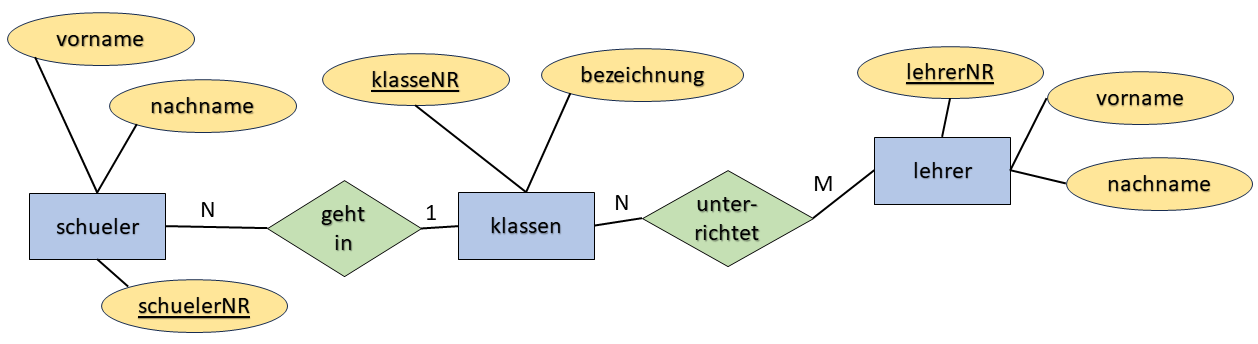
\includegraphics[width=\textwidth]{\pics/Optimierung.png}\\
\end{minipage}
Bildet man jeden Entitätstyp und jede Beziehung als eine eigene Tabelle ab, so erhält man z.B.:
\begin{minipage}{\textwidth}
	\begin{minipage}{0.5\textwidth}
		\begin{tabular}{lll}
			\multicolumn{3}{c}{\lstinline!schueler!}\\
			\hline
			\underline{\lstinline!schuelerNR!}&\lstinline!vorname!&\lstinline!nachname!\\
			\hline
			105&Max&Verstappen\\
			106&Charles&Leclerc\\
			110&Lewis&Hamilton\\
		\end{tabular}
	\end{minipage}
	\begin{minipage}{0.5\textwidth}
		\begin{tabular}{ll}
			\multicolumn{2}{c}{\lstinline!klasse!}\\
			\hline
			\underline{\lstinline!klasseNR!}&\lstinline!bezeichnung!\\
			\hline
			1&BK22\\
			2&BK13\\
		\end{tabular}
	\end{minipage}
\end{minipage}
\begin{minipage}{0.3\textwidth}
	\begin{tabular}{lll}
		\multicolumn{3}{c}{\lstinline!lehrer!}\\
		\hline
		\underline{\lstinline!lehrerNR!}&\lstinline!vorname!&\lstinline!nachname!\\
		\hline
		12&Christian&Horner\\
		13&Frederic&Vasseur\\
	\end{tabular}
\end{minipage}
\begin{minipage}{\textwidth}
	\begin{minipage}{0.5\textwidth}
		\begin{tabular}{ll}
			\multicolumn{2}{c}{\lstinline!schueler_klasse!}\\
			\hline
			\underline{\lstinline!schuelerNR!}&\underline{\lstinline!klasseNR!}\\
			\hline
			105&1\\
			106&1\\
			110&2\\
		\end{tabular}
	\end{minipage}
	\begin{minipage}{0.5\textwidth}
		\begin{tabular}{ll}
			\multicolumn{2}{c}{\lstinline!lehrer_klasse!}\\
			\hline
			\underline{\lstinline!klasseNR!}&\underline{\lstinline!lehrerNR!}\\
			\hline
			1&12\\
			1&13\\
			2&12\\
			2&13\\
		\end{tabular}
	\end{minipage}
\end{minipage}
Die Tabelle \lstinline!schueler_klasse! beschreibt die N:1 Beziehung zwischen den Entitätstypen \lstinline!schueler! und \lstinline!klasse!. Da jedem Schüler genau eine Klasse zugeordnet wird, kann man diese Tabelle einsparen, indem man in der Tabelle Schüler als zusätzliches Attribut den Fremdschlüssel \lstinline!klasseNR! einfügt, die direkt die Klasse angibt, in die der Schüler geht:
\begin{minipage}{\textwidth}
	\begin{minipage}{0.6\textwidth}
		\begin{tabular}{llll}
			\multicolumn{4}{c}{\lstinline!schueler!}\\
			\hline
			\underline{\lstinline!schuelerNR!}&\lstinline!vorname!&\lstinline!nachname!&\lstinline!klasseNR!\\
			\hline
			105&Max&Verstappen&1\\
			106&Charles&Leclerc&1\\
			110&Lewis&Hamilton&2\\
		\end{tabular}
	\end{minipage}
	\begin{minipage}{0.4\textwidth}
		\begin{tabular}{ll}
			\multicolumn{2}{c}{\lstinline!klasse!}\\
			\hline
			\underline{\lstinline!klasseNR!}&\lstinline!bezeichnung!\\
			\hline
			1&BK22\\
			2&BK13\\
		\end{tabular}
	\end{minipage}
\end{minipage}
\begin{minipage}{\textwidth}
	\begin{minipage}{0.5\textwidth}
		\begin{tabular}{lll}
			\multicolumn{3}{c}{\lstinline!lehrer!}\\
			\hline
			\underline{\lstinline!lehrerNR!}&\lstinline!vorname!&\lstinline!nachname!\\
			\hline
			12&Christian&Horner\\
			13&Frederic&Vasseur\\
		\end{tabular}
	\end{minipage}
	\begin{minipage}{0.5\textwidth}
		\begin{tabular}{ll}
			\multicolumn{2}{c}{\lstinline!lehrer_klasse!}\\
			\hline
			\underline{\lstinline!klasseNR!}&\underline{\lstinline!lehrerNR!}\\
			\hline
			1&12\\
			1&13\\
			2&12\\
			2&13\\
		\end{tabular}
	\end{minipage}
\end{minipage}
Die N:M Beziehung zwischen \lstinline!klasse! und \lstinline!lehrer! kann so nicht eingespart werden. Ein Lehrer unterrichtet im Normalfall mehrere Klassen, also müsste man in der Tabelle Klasse mehrere Einträge hinzufügen und umgekehrt wird eine Klasse von mehreren verschiedenen Lehrern unterrichtet.
\begin{Exercise}[title={Überlege dir welche Beziehungstabellen man in Aufgabe \ref{ERMErstellen1} wegoptimieren kann und gib an, welches Attribut man an welchen Entitätstyp als Fremdschlüssel hinzufügen muss.}, label=Optimierung]
\end{Exercise}
%%%%%%%%%%%%%%%%%%%%%%%%%%%%%%%%%%%%%%%%%%
\begin{Answer}[ref=Optimierung]
	\begin{itemize}
		\item Fahrradverleih:\\
		Die Beziehungstabelle zur Beziehung \lstinline!mietet! kann wegoptimiert werden, indem man das Attribut \lstinline!kundenNR! als Fremdschlüssel zur Tabelle \lstinline!fahrrad! hinzufügt.
		\item Autohändler:\\
		Die Beziehungstabelle zur Beziehung \lstinline!gekauft! kann wegoptimiert werden, indem man das Attribut \lstinline!kundenNR! als Fremdschlüssel zur Tabelle \lstinline!auto! hinzufügt.\\
		Die Beziehungstabelle zur Beziehung \lstinline!verfuegt! kann wegoptimiert werden, indem man das Attribut \lstinline!fahrzeugID! als Fremdschlüssel zur Tabelle \lstinline!reifen! hinzufügt.
		\item DVD-Verleih:\\
		Die Beziehungstabelle zur Beziehung \lstinline!arbeitet_in! kann wegoptimiert werden, indem man das Attribut \lstinline!filiale.id! als Fremdschlüssel zur Tabelle \lstinline!mitarbeiter! hinzufügt.
	\end{itemize}
\end{Answer}
	\newpage
	% !TeX root = ../Skript_DB.tex
\cohead{\Large\textbf{Datentypen}}
\subsection{Datentypen}
Eine relationale Datenbank besteht aus verschiedenen \textcolor{red}{Entitätstypen} und \textcolor{red}{Beziehungen} zwischen diesen, die jeweils als Tabellen abgebildet werden. Die \textcolor{red}{Entitätstypen} und \textcolor{red}{Beziehungen} sind dabei sozusagen die Überschriften der Tabellen, die einzelnen Spalten bezeichnet man als \textcolor{blue}{Attribute} und die Zeilen als Entitäten:

\begin{table}[h]
	\centering
	\begin{tabular}{llll}
		\multicolumn{4}{c}{\textcolor{red}{\textbf{Schüler}}}\\
		\textcolor{blue}{\underline{schNr}} 	& \textcolor{blue}{vorname} 	& \textcolor{blue}{nachname}	& \textcolor{blue}{alter}  \\
		\midrule
		23&Heinz&Huber&15\\
		24&Max&Power&NULL\\
	\end{tabular}
\end{table}
\textcolor{red}{Schüler} ist hier der \textcolor{red}{Entitätstyp} mit den \textcolor{blue}{Attributen schNr, vorname, nachname} und \textcolor{blue}{alter}. Der Schüler mit der \textcolor{blue}{schNr} 23, Heinz, Huber, 15 ist eine Entität.
Datenbanken benötigten meist bereits beim Erstellen eines \textcolor{red}{Entitätstyps}/Tabelle eine Angabe zum Datentyp der jeweiligen Attribute. Wir beschränken uns hier auf wenige "große" Datentypen. Je nach Datenbankmanagementsystem lassen sich die Datentypen nochmals in mehrere kleinere Untertypen aufspalten.
SQLite ist ein beliebtes DBMS, da es klein und relativ simpel ist. Wir werden selbst mit SQLite arbeiten, weil außerdem eine portable Version gibt. SQLite beschränkt sich darüber hinaus bereits selbst auf wenige Datentypen:
\begin{tcolorbox}[title=Datentypen]
	\begin{itemize}
		\item INTEGER (ganze Zahl)
		\item REAL (oft auch float genannt, Flließkommazahl)
		\item TEXT (oft auch char oder string genannt)
		\item BLOB
		\item DATE/DATETIME (Anmerkung: SQLite hat hierfür keinen eigenen Datentyp, die meisten DBMS jedoch schon. SQLite speichert ein Datum als Text oder Zahl ab)
	\end{itemize}
\end{tcolorbox}

\begin{Exercise}[title={Beantworte folgende Fragen; Du kannst das Internet zu Rate ziehen.}, label=Datentypen]
	\begin{enumerate}
		\item Informiere dich über den NULL-Wert, der oben in der Datenbank vorkommt. Für was steht dieser Wert? Was ist der Unterschied zwischen Null bzw. 0 und NULL?
		\item Was ist ein Byte?
		\item Wie werden INTEGER auf der Datenbank gespeichert?
	\end{enumerate}
\end{Exercise}
%%%%%%%%%%%%%%%%%%%%%%%%%%%%%%%%%%%%%%%%%
\begin{Answer}[ref=Datentypen]
	\begin{enumerate}
		\item Informiere dich über den NULL-Wert, der oben in der Datenbank vorkommt. Für was steht dieser Wert? Was ist der Unterschied zwischen Null bzw. 0 und NULL?

		Der Wert NULL bedeutet, dass kein Wert vorhanden ist. Ein ähnliches Konzept kennen wir aus der Mathematik. Die Gleichung \(x^2=0\) hat die Lösung \(x=0\), während die Gleichung \(x^2=-1\) keine Lösung hat, was wir durch das Blitzsymbol \Lightning\normalsize anzeigen. Im obigen Beispiel steht ein Wert von 0 für das Alter für eine Person, die ihren ersten Geburtstag noch nicht hatte. Ein Wert von NULL bedeutet, dass das Alter unbekannt ist.
		\item Was ist ein Byte?

		Ein Byte ist eine Informationseinheit, die normalerweise aus 8 Bit besteht. Ein Bit kann die beiden Zustände 1 oder 0 annehmen. Ein Byte kann also \(2^8=256\) verschiedene Zustände annehmen. Ältere Zeichensätze haben jeweils ein Zeichen in ein Byte gespeichert. So konnten also 256 verschiedene Zeichen (z.B. a, b, c, A, B, C, §, +, usw.) unterschieden werden.
		\item Wie werden INTEGER auf der Datenbank gespeichert?

		Im Alltag verwenden wir das Dezimalsystem, d.h. jede Zahl wird in Form von Potenzen von 10 dargestellt:

		\(123=1\cdot10^2+2\cdot 10^1+3\cdot 10^0=100+20+3\)

		INTEGER werden einfach vom Dezimalsystem auf das Binärsystem übertragen:

		\(123=1111011_{BIN}=1\cdot2^6+1\cdot2^5+1\cdot2^4+0\cdot2^3+1\cdot2^2+1\cdot2^1+1\cdot2^0\)

		\(=64+32+16+8+2+1=123\).

		Das erste Bit kann als Vorzeichen verwendet werden. Dann kann man in einem Byte Zahlen von \(-128\) bis \(127\) speichern. Je mehr Byte man für eine Zahl verwendet, desto mehr Speicherplatz benötigt man. Jedoch lassen sich dann auch größere Zahlen speichern.
	\end{enumerate}
\end{Answer}
	\newpage
	%%%%%%%%%%%%%%%%%%%%%%%%%%%%%%%%%%%%%%%%%%%%%%%%%%%
	\rohead{DBMS und SQL}
	% !TeX root = ../Skript_DB.tex
\cohead{\Large\textbf{DBMS und SQL}}
\section[DBMS und SQL]{Datenbankmanagementsystem und Structured Query Language}
\subsection{Begriffe}
In einer Datenbank werden Daten oder auch Informationen abgelegt. Für das Erstellen, Ändern oder auch für die Abfrage von Daten benötigt man ein Programm, das sogenannte Datenbankmanagementsystem. So wie es verschiedene Tabellenkalkulationsprogramme wie z.B. Excel, Calc oder Numbers gibt, stehen  verschiedene DBMS wie z.B. Oracle, Postgres oder DB2 zur Auswahl.

Obwohl es kleinere Unterschiede vor allem im Design der Oberfläche gibt, funktionieren alle Tabellenkalkulationsprogramme in großen Teilen gleich, z.B. summiert \lstinline!SUM(A1; B3; C5)! die Werte der angegebenen Zellen zusammen. Etwas ähnliches gibt es für DBMS ebenfalls. Fast alle DBMS verwenden SQL bzw. Structured Query Language für das Verwalten der Datenbank. Will man z.B. eine neue Tabelle in der Datenbank erstellen, so kann man nicht einfach auf \textit{Neu} in einer Oberfläche klicken, so wie man z.B. in Word ein neues Dokument erstellen kann, sondern muss dem DBMS eine Anweisung in Textform als SQL-Befehl geben, wie z.B.
 \lstinline!CREATE TABLE farben(laufendeNR INT PRIMARY KEY, bezeichnung TEXT,!

\lstinline!rotanteil INT NOT NULL, blauanteil INT NOT NULL, gruenanteil NOT NULL);!.
In obiger Tabelle kann man dann Farben in der RGB-Darstellung speichern.

Ein sehr entfernt ähnliches Konzept haben wir bei HTML mit den verschiedenen Tags kennengelernt.

SQL selbst ist nicht case sensitive, d.h. die Groß- und Kleinschreibung spielt keine Rolle. Jedoch hat es sich eingebürgert die SQL-Schlüsselwörter komplett in Großbuchstaben zu schreiben und die Bezeichnungen von Tabellen/Entitäten und Attributen klein zuschreiben. Jeder SQL-Befehlt endet mit einem Strichpunkt.

Wir werden als DBMS SQLite verwenden, da es nicht viel Speicherplatz braucht und es eine portable Version gibt, d.h. es ist keine Installation notwendig. SQLite kann man starten, indem man die \texttt{sqlite3.exe} startet.

\begin{figure}[h]
	\centering
	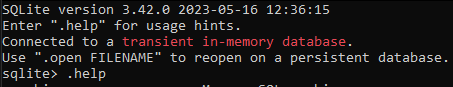
\includegraphics[]{\pics/sqliteStart.png}
	\caption*{Kommandozeile nach dem Starten von \texttt{sqlite3.exe}.}
\end{figure}
Alle SQLite-Befehle (diese sind keine SQL-Befehle) beginnen mit einem Punkt. Für Interessierte: Der Befehl \lstinline!.help! gibt eine Übersicht der möglichen Befehle. Wir werden aber nur wenige Befehle, wie z.B. \lstinline!.open bsp.db! verwenden.
	\newpage
	% !TeX root = ../Skript_DB.tex
\cohead{\Large\textbf{Anlegen einer DB}}
\cohead{\Large\textbf{Anlegen/Befüllen einer DB}}
\subsection[Anlegen/Befüllen einer DB]{SQL - Anlegen und Befüllen einer Datenbank}
Erinnerung: Wir werden das Programm SQLite als Datenbankmanagementsystem (DBMS) verwenden. Nach dem Starten von SQLite sind nur noch SQLite-spezifische Befehle, die immer mit einem Punkt beginnen oder SQL-Anweisungen erlaubt.

\subsection{Erstellen bzw. Öffnen einer Datenbank}

\medskip

\begin{minipage}{\textwidth}
    \adjustbox{valign=t, padding=0ex 0ex 2ex 0ex}{\begin{minipage}{\textwidth-6.91cm-2ex}\raggedright
        Starte die \texttt{sqlite3.exe}. Mit dem Befehl \lstinline!.open #Name#.db! (z.B. \lstinline!.open meineDatenbank.db!) lässt sich eine bestehende DB öffnen bzw. neu erstellen. Im Verzeichnis, in dem auch \texttt{sqlite3.exe} liegt, sollte nun (falls zuvor noch nicht vorhanden) eine neue Datei \texttt{\#Name\#.db} erstellt worden sein.

        Mit dem Befehl \lstinline!.tables! kann man sich alle in der DB vorhandenen Tabellen/Entitätstypen anzeigen lassen.
    \end{minipage}}%
    \adjustbox{valign=t}{\begin{minipage}{6.91cm}
            \centering
            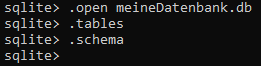
\includegraphics[width=\textwidth]{\pics/createDB.png}
            Da noch keine Tabellen angelegt sind, geben die Befehle \lstinline!.tables! und \lstinline!.schema! keine Ausgabe zurück.
    \end{minipage}}%
\end{minipage}

\medskip

Mit dem Befehl \lstinline!.schema! kann man sich die Tabellen mit einer Liste der Attribute anzeigen lassen.
\begin{tcolorbox}[title=Datenbank öffnen]
	Starte \texttt{sqlite3.exe} und gib dann \lstinline!.open datenbankname.db! ein.
\end{tcolorbox}

\subsection{Erstellen bzw. löschen von Tabellen/Entitätstypen}
Neue Tabellen/Entitätstypen lassen sich mit dem SQL-Befehl \lstinline!CREATE TABLE! erzeugen:

\begin{tcolorbox}[title=Tabellen erstellen]
	\lstinline!CREATE TABLE name_tabelle (name_attribut1 datentyp1 einschränkung1,!

    \lstinline!name_attribut2 datentyp2 einschränkung2, ...);!
\end{tcolorbox}
\textcolor{red}{ACHTUNG: Bei SQL-Befehlen den Strichpunkt am Ende der Zeile nicht vergessen!} Man kann SQL-Befehle auch auf mehrere Zeilen aufteilen.

Als Datentypen werden wir \lstinline!INT! für ganze Zahlen und \lstinline!TEXT! für Texte oder Geburtsdaten verwenden. Dem interessierten Leser seien die restlichen Datentypen zum Selbststudium ans Herz gelegt.

Als Einschränkungen werden wir uns auf \lstinline!PRIMARY KEY! und \lstinline!NOT NULL! beschränken. \lstinline!PRIMARY KEY! markiert das Attribut als Primärschlüssel und sollte als erstes Attribut angelegt werden. \lstinline!NOT NULL! zeigt an, dass dieses Attribut beim Füllen der Tabelle mit Daten nicht leer bleiben darf. Die Angabe von Einschränkungen ist optional.

Bestehende Tabellen lassen sich mit dem Befehl \lstinline!DROP TABLE name_tabelle! wieder löschen:
\begin{tcolorbox}[title=Tabellen löschen]
	\lstinline[breaklines=true]!DROP TABLE name_tabelle !
\end{tcolorbox}
\begin{figure}[h]
	\centering
	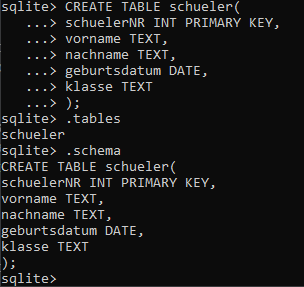
\includegraphics[]{\pics/createTable_schueler.png}
	\caption*{Die Tabelle \lstinline!schueler! wurde angelegt. Die Befehle \lstinline!.tables! und \lstinline!.schema! haben nun einen Rückgabewert.}
\end{figure}
\begin{figure}[h]
	\centering
	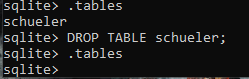
\includegraphics[]{\pics/dropTabel_schueler.png}
	\caption*{Die Tabelle \lstinline!schueler! wurde gelöscht.}
\end{figure}

\subsection{Befüllen einer Tabelle mit Daten}
Um einer Tabelle eine neue Entität/Zeile hinzuzufügen, verwendet man den \lstinline!INSERT INTO! Befehl:

\begin{tcolorbox}[title=Befüllen einer Tabelle]
    Werte für alle Attribute vorhanden:

	\lstinline!INSERT INTO name_tabelle VALUES(wert1, wert2, wert3,...);!

    Nur bestimmte Attribute sollen mit Werten belegt werden:

    \lstinline!INSERT INTO name_tabelle(attribut1, attribut3,...)VALUES(wert1, wert3,...);!
\end{tcolorbox}
\begin{itemize}
	\item Alle Attribute angegeben: Sollen für alle Attribute Werte angegeben werden, so kann man einfach die Werte als kommaseparierte Liste angeben:\\
	\lstinline!INSERT INTO schueler VALUES(1,'Heinz','Huber','01.01.2000','BKFH');!

	Beachte, dass Texte mit Anführungszeichen (auf der Tastatur beim \#-Zeichen) angegeben werden müssen.
	\item Manche Attribute ohne Wert: Hat man für manche Attribute keinen Wert zur Hand, so kann man die Entität trotzdem anlegen, indem man hinter den Namen der Entität die Liste der Attribute angibt, für die man Werte zur Hand hat:

	\lstinline!INSERT INTO schueler(schuelerNR, vorname, nachname, klasse) VALUES (20,!

	\lstinline!'Anton', 'Atonovich', 'BK11');!
\end{itemize}

\begin{Exercise}[title={Beantworte folgende Fragen mit Hilfe deiner Datenbank.}, label=Befuellen]
	\begin{enumerate}
		\item Erzeuge eine Tabelle \lstinline!schueler! mit den Attributen \lstinline!schuelerNR! als Primärschlüssel, der nicht NULL sein darf, \lstinline!name!, \lstinline!plz! und \lstinline!klasse!.
		\item Füge 2 verschiedene Schüler hinzu, die aus den Klassen BK13 und BK21 stammen.
		\item Was passiert, wenn man einen weiteren Schüler mit einer bereits vergebenen \lstinline!schuelerNR! hinzufügen will?
		\item Was passiert, wenn man einen weiteren Schüler einfügen will ohne eine \lstinline!schuelerNR! anzugeben?
		\item Wie sehen die Ausgaben von \lstinline!.tables! und \lstinline!.schema! aus?
	\end{enumerate}
\end{Exercise}
%%%%%%%%%%%%%%%%%%%%%%%%%%%%%%%%%%%%%%%%%
\begin{Answer}[ref=Befuellen]
	\begin{enumerate}
		\item Erzeuge eine Tabelle \lstinline!schueler! mit den Attributen \lstinline!schuelerNR! als Primärschlüssel, der nicht NULL sein darf, \lstinline!name!, \lstinline!plz! und \lstinline!klasse!.

		\lstinline[breaklines=true]!CREATE TABLE schueler(schuelerNR INT PRIMARY KEY NOT NULL, name TEXT, plz INT, klasse TEXT);!
		\item Füge 2 verschiedene Schüler hinzu, die aus den Klassen BK13 und BK21 stammen., z.B.:

		\lstinline!INSERT INTO schueler VALUES (1, 'Heinz Huber', 70180, 'BK13');!

		\lstinline!INSERT INTO schueler VALUES (2, 'Dasan Ilhan', 70567, 'BK21');!

		\item Was passiert, wenn man einen weiteren Schüler mit einer bereits vergebenen schuelerNR hinzufügen will?

		Z.B. folgender Befehl: \lstinline!INSERT INTO schueler VALUES (1, 'Alina Lutz', 70874, 'BK21');!
		Es wird ein Fehler ausgegeben: \lstinline!Runtime error: UNIQUE constraint failed: schueler.schuelerNR!

		Unique bedeutet einzigartig und constraint steht für Einschränkung. Der Fehler besagt also, dass beim Hinzufügen eines Schülers in der Tabelle \lstinline!schueler! der Wert des Attributs \lstinline!schuelerNR! nicht einzigartig war.
		\item Was passiert, wenn man einen weiteren Schüler mit der schuelerNR NULL einfügen will?

		Z.B. folgender Befehl: \lstinline!INSERT INTO schueler(name) VALUES ('Vanessa Oranbay');!. Dieser Befehl würde gerne eine Zeile in der Tabelle \lstinline!schueler! anlegen, bei der alle Einträge bis auf den \lstinline!name! den Wert NULL haben.
		Es wird ein Fehler ausgegeben: \lstinline!Runtime error: NOT NULL constraint failed: schueler.schuelerNR!

		Der Fehler besagt also, dass beim Hinzufügen eines Schülers in der Tabelle \lstinline!schueler! der Wert des Attributs \lstinline!schuelerNR! NULL war, was nicht erlaubt ist.
		\item Wie sehen die Ausgaben von .tables und .schema aus?

		\lstinline!sqlite> .table!

		\lstinline!schueler!

		\lstinline!sqlite> .schema!

		\lstinline!CREATE TABLE schueler(schuelerNR INT PRIMARY KEY NOT NULL,!

		\lstinline!name TEXT, plz INT, klasse TEXT);!

        .tables gibt also nur die Namen der Tabellen aus und .schema gibt zusätzlich den SQL-Befehl zum erstellen der Tabellen aus. So lassen sich die Attribute mit ihren jeweiligen Einschränkungen und Datentypen ablesen.
	\end{enumerate}
\end{Answer}
	\newpage
	\cohead{\Large\textbf{SELECT-Statement}}
\subsection[SELECT-Statement]{SQL - Das SELECT-Statement}
Speichere die Datei \texttt{vieleSchueler.db} in deinem Verzeichnis und öffne die DB mit \texttt{sqlite3.exe} (\lstinline!.open vieleSchueler.db!). Mit dem Befehl \lstinline!.tables! oder \lstinline!.schema! kannst du dir die Tabellen (mit Attributen) anzeigen lassen.\\
Wie erwartet gibt es eine Tabelle \lstinline!schueler!. Um den Inhalt anzuzeigen, kannst du das SELECT-Statement von SQL verwenden:
\begin{tcolorbox}[title=SELECT-Statement]
	\lstinline!SELECT * FROM schueler;!
\end{tcolorbox}
Mit den Zusätzen \lstinline!ORDER BY nachname ASC! bzw. \lstinline!ORDER BY nachname DESC!  kannst du die Ausgabe nach einem Attribut aufsteigend (ascending) bzw. absteigend (descending) sortieren lassen. Ohne die Angabe von \lstinline!ASC! bzw. \lstinline!DESC! erfolgt die Ausgabe standardmäßig aufsteigend.

\begin{Exercise}[title={Beantworte folgende Fragen mit Hilfe deiner Datenbank und dem Internet.}, label=Select]
	\begin{enumerate}
		\item Welche Ausgabe erzeugt das Statement \lstinline!SELECT * FROM schueler;!?
		\item Wofür steht der Stern (\lstinline!*!) in obigem Statement?
		\item Welche Ausgabe erzeugt \lstinline!SELECT vorname, nachname FROM schueler;!?
		\item Finde ein Statement, um dir \lstinline!nachname!, \lstinline!plz! und \lstinline!klasse! anzeigen zu lassen.
	\end{enumerate}
\end{Exercise}
%%%%%%%%%%%%%%%%%%%%%%%%%%%%%%%%%%%%%%%%%
\begin{Answer}[ref=Select]
	\begin{enumerate}
		\item Welche Ausgabe erzeugt das Statement \lstinline!SELECT * FROM schueler;!?\\
		Das Statement gibt alle in der Tabelle vorhandenen Schüler aus:\\
		\begin{lstlisting}
			1|Anica|Nosudohein|6268|06.11.1998|BKFH
			2|Marlies|Gavofu|25361|06.01.2002|BK2
			3|Franz|Rotagateson|71296|13.01.1998|BK1
			4|Elisabeth|Kotibodoweiner|14798|20.11.2003|BK1
			5|Henni|Kitavare|22926|21.07.1999|BK2
			6|Mariana|Hewalode|23879|19.05.2004|BK2
			7|Henry|Zütuschatthein|94405|31.12.2004|BK1
			8|Fatma|Varobason|19370|08.01.2005|BK1
			9|Gundel|Culufledemeiner|97896|12.04.1996|BKFH
			10|Reinhold|Tulimattson|25821|08.08.1997|BK1
			11|Silvia|Cüwiwattemüller|88339|09.11.2001|BK2
			...\end{lstlisting}
		Anmerkung: Es wurden aus Platzgründen nicht alle Schüler hier aufgelistet.
		\item Wofür steht der Stern (\lstinline!*!) in obigem Statement?\\
		Der Stern ist eine sogenannte Wildcard. Das SELECT-Statement muss wissen, welche Attribute angezeigt werden sollen. Der Stern bedeutet, dass die Werte aller an der Tabelle vorhandenen Attribute ausgegeben werden.
		\item Welche Ausgabe erzeugt \lstinline!SELECT vorname, nachname FROM schueler;!?
		\begin{lstlisting}
			Anica|Nosudohein
			Marlies|Gavofu
			Franz|Rotagateson
			Elisabeth|Kotibodoweiner
			Henni|Kitavare
			Mariana|Hewalode
			Henry|Zütuschatthein
			Fatma|Varobason
			Gundel|Culufledemeiner
			Reinhold|Tulimattson
			Silvia|Cüwiwattemüller
			...\end{lstlisting}
		Da nun nicht mehr der Stern verwendet wurde, um die Werte aller Attribute anzuzeigen, werden nur die Werte von \lstinline!vorname! und \lstinline!nachname! angezeigt.
		\item Finde ein Statement, um dir \lstinline!nachname!, \lstinline!plz! und \lstinline!klasse! anzeigen zu lassen.\\
		\lstinline!SELECT nachname, plz, klasse FROM schueler;!
	\end{enumerate}
\end{Answer}
	\newpage
	\cohead{\Large\textbf{WHERE-Klausel}}
\subsection[WHERE-Klausel]{SQL - Die WHERE-Klausel}
Im letzten Abschnitt haben wir gelernt, wie wir alle Einträge einer ganzen Tabelle oder eines/mehrerer Attribute anzeigen lassen können. Oft sind die Tabellen jedoch so groß, dass es sehr mühsam wäre, alle Einträge von Hand zu durchsuchen. Daher kann man das SELECT-Statement mit Hilfe der WHERE-Klausel einschränken. Die WHERE-Klausel kann auch an viele andere Statements angehängt werden, wie z.B. beim später noch einzuführenden DELETE-Statement.\\
Der grundsätzliche Aufbau ist denkbar einfach:
\begin{tcolorbox}[title=WHERE-Klausel]
	\lstinline!SQL-STATEMENT WHERE bedingungen;!
\end{tcolorbox}
Der Teufel steckt wie so oft im Detail, hier im Aufbau der Bedingungen. Einige wichtige Beispiele:
\begin{itemize}
	\item \lstinline!=! gleich, \lstinline!<! kleiner, \lstinline!>! größer, \lstinline!<=! kleiner gleich, \lstinline!>=! größer gleich, \lstinline&!=& ungleich\\
	Insbesondere für den Vergleich von Attributen mit dem Datentyp INT geeignet.\\
	Beispiel: \lstinline!SELECT * FROM schueler where schuelerNR<=10;! gibt alle Schueler, deren \lstinline!schuelerNR! kleiner oder gleich 10 ist aus.
	\item \lstinline!IS! bzw. \lstinline!IS NOT!\\
	Wird normalerweise für den Vergleich für Attribute mit dem Datentyp \lstinline!TEXT! verwendet und fungiert dort wie ein Gleichzeichen bzw. Ungleichzeichen.\\
	Beispiele: 	\lstinline!SELECT * FROM schueler WHERE vorname IS 'Carsten';! gibt alle Schueler aus, deren \lstinline!vorname! Carsten ist.\\
	Hinweis: NULL kann als Wert verwendet werden: \lstinline!SELECT * FROM schueler WHERE geburtsdatum IS NULL;! gibt alle Schüler aus, die beim Attribut \lstinline!geburtsdatum! keinen Wert eingetragen haben. (Es sollten fünf Schüler ohne Geburtsdatum vorhanden sein.)
	\item \lstinline!LIKE muster!\\
	Wird normalerweise für den Vergleich für Attributen mit dem Datentyp \lstinline!TEXT! verwendet. Für das Muster gibt man einen Text mit Platzhaltern an. Das Prozentzeichen steht für beliebig viele (Null oder mehr Zeichen), der Unterstrich für genau ein Zeichen. Beispiele:\\
	\lstinline!SELECT * FROM schueler WHERE vorname LIKE 'A%';!\\
	Gibt alle Schüler aus, deren \lstinline!vorname! mit einem A beginnt.\\
	\lstinline!SELECT * FROM schueler WHERE vorname LIKE 'A%i';!\\
	Gibt alle Schüler aus, deren \lstinline!vorname! mit einem A beginnt und einem i endet (eine Schülerin).
	\lstinline!SELECT * FROM schueler WHERE vorname LIKE 'A___';!\\
	Gibt alle Schüler aus, deren \lstinline!vorname! mit einem A beginnt und insgesamt genau vier Zeichen lang ist (2 Schüler).\\
	\lstinline!SELECT * FROM schueler WHERE nachname LIKE 'Sch___';!\\
	Gib alle Schüler aus, deren \lstinline!nachname! mit Sch beginnt und genau 6 Zeichen hat (ein Schüler).
	\item \lstinline!IN!\\
	Funktioniert wie mehrere Tests auf Gleichheit (\lstinline!=! oder \lstinline!IS!). Die Vergleichswerte werden als kommaseparierte Liste angegeben:\\
	\lstinline!SELECT * FROM schueler WHERE schuelerNR in (1,2,5);!\\
	Gibt die Schüler mit den \lstinline!schuelerNR! 1, 2 und 5 aus.\\
	\lstinline!SELECT * FROM schueler WHERE nachname IN ('Mayer', 'Maier');!\\
	Gibt alle Schüler aus, deren \lstinline!nachname! Mayer oder Maier lautet.
	\item \lstinline!BETWEEN!\\
	Dem \lstinline!IN! sehr ähnlich, diesmal kann man jedoch gleich auf einen ganzen Bereich prüfen:\\
	\lstinline!SELECT * FROM schueler WHERE schuelerNR BETWEEN 10 AND 20;!\\
	Gibt alle Schüler aus, deren \lstinline!schuelerNR! zwischen 10 und 20 liegen (10 und 20 jeweils eingeschlossen).
\end{itemize}
\textcolor{red}{ACHTUNG:} Beim Test auf NULL muss immer \lstinline!IS! statt \lstinline!=! verwendet werden, z.B. liefert \lstinline!SELECT * FROM schueler WHERE plz is NULL;! einen Schüler, während \lstinline!SELECT * FROM schueler WHERE plz = NULL;! kein Ergebnis aber auch keine Fehlermeldung liefert.\\
Es lassen sich mehrere Bedingungen mit einem \lstinline!AND! bzw. \lstinline!OR! verknüpfen:\\
\lstinline!SELECT * FROM schueler WHERE schuelerNR BETWEEN 10 AND 20!
\lstinline!OR nachname IN ('Mayer', 'Maier');!\\
Gibt alle Schüler aus, deren \lstinline!schuelerNR! zwischen 10 und 20 liegen oder deren \lstinline!nachname! Mayer oder Maier lautet.\\
\lstinline!SELECT * FROM schueler WHERE schuelerNR BETWEEN 10 AND 20!
\lstinline!AND nachname IN ('Mayer', 'Maier');!\\
Gibt alle Schüler aus, deren \lstinline!schuelerNR! zwischen 10 und 20 liegen und deren \lstinline!nachname! Mayer oder Maier lautet. (Nur eine Schülerin erfüllt beide Bedingungen gleichzeitig.)\\
\begin{Exercise}[title={Erstelle ein SELECT-Statement mit WHERE-Klausel, das}, label=Where]
	\begin{enumerate}
		\item den Schüler mit der \lstinline!schuelerNR! 31 zurück gibt.
		\item alle Schüler mit der \lstinline!schuelerNR! 10, 23, 50 und 65 findet.
		\item alle Schüler findet, deren \lstinline!nachname! auf hein endet.
		\item alle Schüler findet, deren \lstinline!nachname! nicht auf hein endet.
		\item den Schüler findet, für den keine \lstinline!klasse! angegeben worden ist.
		\item alle Schüler findet, deren \lstinline!schuelerNR! kleiner 18 ist.
		\item alle Schüler findet, deren \lstinline!vorname! aus genau 4 Buchstaben besteht.
		\item Bonus-Frage: Warum gibt das Statement \lstinline!SELECT * FROM schueler WHERE geburtsdatum BETWEEN '01.01.2000' AND '31.12.2000';! viel zu viele Schüler zurück?\\
		Tipp: Probiere das Statement \lstinline!SELECT * FROM schueler WHERE geburtsdatum BETWEEN '31.01.2000' AND '31.12.2000';! oder das Statement \lstinline!SELECT geburtsdatum FROM schueler ORDER BY geburtsdatum;! aus.\\
	\end{enumerate}
\end{Exercise}
%%%%%%%%%%%%%%%%%%%%%%%%%%%%%%%%%%%%%%%%%
\begin{Answer}[ref=Where]
	\begin{enumerate}
		\item den Schüler mit der \lstinline!schuelerNR! 31 zurück gibt.\\
		\lstinline!SELECT * FROM schueler WHERE schuelerNR = 31;!
		\item alle Schüler mit der \lstinline!schuelerNR! 10, 23, 50 und 65 findet.\\
		\lstinline!SELECT * FROM schueler WHERE schuelerNR in (10, 23, 50, 65);!
		\item alle Schüler findet, deren \lstinline!nachname! auf hein endet.\\
		\lstinline!SELECT * FROM schueler WHERE nachname LIKE '%hein';!
		\item alle Schüler findet, deren \lstinline!nachname! nicht auf hein endet.\\
		\lstinline!SELECT * FROM schueler WHERE nachname NOT LIKE '%hein';!
		\item alle Schüler findet, für die keine \lstinline!klasse! angegeben worden ist.\\
		\lstinline!SELECT * FROM schueler WHERE klasse IS NULL;!\\
		\item alle Schüler findet, deren \lstinline!schuelerNR! kleiner 18 ist.\\
		\lstinline!SELECT * FROM schueler WHERE schuelerNR < 18;!
		\item alle Schüler findet, deren \lstinline!vorname! aus genau 4 Buchstaben besteht.\\
		\lstinline!SELECT * FROM schueler WHERE vorname LIKE '____';!
		\item Bonus-Frage: Warum gibt das Statement \lstinline!SELECT * FROM schueler WHERE geburtsdatum BETWEEN '01.01.2000' AND '31.12.2000';! viel zu viele Schüler zurück?\\
		Tipp: Probiere das Statement \lstinline!SELECT * FROM schueler WHERE geburtsdatum BETWEEN '31.01.2000' AND '31.12.2000';! oder das Statement \lstinline!SELECT geburtsdatum FROM schueler ORDER BY geburtsdatum;! aus.\\
		Das zweite Statement aus dem Tipp zeigt, dass die Geburtsdaten nicht wie erwartet sortiert werden, sondern Zeichen für Zeichen. Da die Punkte bei allen Geburtsdaten an der gleichen Stelle stehen, können wir diese ignorieren. Man kann sich die Geburtsdaten dann einfach als Zahlen vorstellen, z.B. wäre 01.04.1995 die Zahl 1.041.995. Nun werden alle \lstinline!schueler! mit Geburtsdaten, deren Zahl zw. 1.012.000 und 31.122.000 liegen, zurückgegeben. Z.B. enspricht das Geburtsdatum der Schülerin mit \lstinline!schuelerNR! 100 10.07.1997 der Zahl 10.071.997. Da diese Zahl zwischen den beiden Grenzen 1.012.000 und 31.122.000 liegt, wird sie \textit{fälschlicherweise} ausgegeben.
	\end{enumerate}
\end{Answer}
	\newpage
	% !TeX root = ../Skript_DB.tex
\cohead{\Large\textbf{DELETE/UPDATE-Statement}}
\subsection[DELETE-Statement]{SQL - Das DELETE-Statement}\label{delete}
Mit Hilfe des DELETE-Statements lassen sich Einträge aus einer Tabelle löschen (Das DROP-Statement war zum Löschen der kompletten Tabelle. Eine Verwechslung der beiden Statements sollte aus offensichtlichen Gründen vermieden werden):
\begin{tcolorbox}[title=DELETE-Statement]
	\lstinline!DELETE FROM name_der_Tabelle WHERE bedingungen;!
\end{tcolorbox}
\textcolor{red}{ACHTUNG: Vergisst man die WHERE-Klausel oder wählt mit der WHERE-Klausel mehr Einträge aus als beabsichtigt, werden ALLE oder mehr Einträge als beabsichtigt gelöscht.}

\begin{Exercise}[title={Lösche folgende Einträge aus der Datenbank:}, label=Delete]
	\begin{enumerate}
		\item Den Schüler mit der \lstinline!schuelerNR! 40.
		\item Alle Schüler mit der \lstinline!schuelerNR! 10, 20, 50 und 60.
		\item Alle Schüler, deren \lstinline!vorname! auf \textit{ia} endet.
	\end{enumerate}
\end{Exercise}
%%%%%%%%%%%%%%%%%%%%%%%%%%%%%%%%%%%%%%%%%
\begin{Answer}[ref=Delete]
	\begin{enumerate}
		\item Den Schüler mit der \lstinline!schuelerNR! 40.

		\lstinline!DELETE FROM schueler WHERE schuelerNR = 40;!
		\item Alle Schüler mit der \lstinline!schuelerNR! 10, 20, 50 und 60.

		\lstinline!DELETE FROM schueler WHERE schuelerNR IN (10, 20, 50, 60);!
		\item Alle Schüler, deren \lstinline!vorname! auf \textit{ia} endet.

		\lstinline!DELETE FROM schueler WHERE vorname LIKE '%ia';!
	\end{enumerate}
\end{Answer}
	% !TeX root = ../Skript_DB.tex
\cohead{\Large\textbf{DELETE/UPDATE-Statement}}
\subsection[UPDATE-Statement]{SQL - Das UPDATE-Statement}\label{update}
Mit Hilfe des UPDATE-Statements lassen sich einzelne Werte eines Eintrags in einer Tabelle nachträglich ändern:
\begin{tcolorbox}[title=UPDATE-Statement]
	\lstinline[breaklines=true]!UPDATE name_der_Tabelle SET attribut1=wert1, attribut2=wert2, ... WHERE bedingungen;!
\end{tcolorbox}
\textcolor{red}{ACHTUNG: Vergisst man die WHERE-Klausel oder wählt mit der WHERE-Klausel mehr Einträge aus als beabsichtigt, werden ALLE oder mehr Einträge als beabsichtigt geändert.}
\begin{Exercise}[title={Ändere folgende Einträge aus der Datenbank:}, label=Update]
	\begin{enumerate}
		\item Der Schüler mit der \lstinline!schuelerNR! 19 soll mit \lstinline!vornamen! Hans Gustav Adalbert heißen.
		\item Die Bezeichnung der \lstinline!klasse! soll von BK2 auf BK22 geändert werden.
		\item Bei einigen Schülern ist ein Problem beim Eintragen der \lstinline!plz! aufgetreten. Bei allen Schülern mit einer 4-stelligen \lstinline!plz! soll diese auf NULL geändert werden.
	\end{enumerate}
\end{Exercise}
%%%%%%%%%%%%%%%%%%%%%%%%%%%%%%%%%%%%%%%%%
\begin{Answer}[ref=Update]
	\begin{enumerate}
		\item Der Schüler mit der \lstinline!schuelerNR! 19 soll mit \lstinline!vornamen! Hans Gustav Adalbert heißen.

		\lstinline!UPDATE schueler SET vorname = 'Hans Gustav Adalbert' WHERE schuelerNR = 19;!
		\item Die Bezeichnung der \lstinline!klasse! soll von BK2 auf BK22 geändert werden.

		\lstinline!UPDATE schueler SET klasse = 'BK22' WHERE klasse IS 'BK2';!
		\item Bei einigen Schülern ist ein Problem beim Eintragen der \lstinline!plz! aufgetreten. Bei allen Schülern mit einer 4-stelligen \lstinline!plz! soll diese auf NULL geändert werden.

		\lstinline!UPDATE schueler SET plz = NULL WHERE plz < 10000;!
	\end{enumerate}
\end{Answer}
	\newpage
	% !TeX root = ../Skript_DB.tex
\cohead{\Large\textbf{Funktionen}}
\subsection[Funktionen]{Funktionen im SELECT-Statement}\label{funktionen}
Öffne die Datenbank \texttt{schule.db} mit dem Datenbank-Browser oder sqlite3.exe.

SQL bietet einige einfache Funktionen an, die man innerhalb des SELECT-Statements verwenden kann:
\begin{tcolorbox}[title=Funktionen in SQL]
	\lstinline!SELECT FUNKTIONSNAME(name_attribut) FROM name_tabelle (WHERE bedingungen);!
\end{tcolorbox}
\begin{itemize}
	\item \lstinline!COUNT!	Anzahl der Werte zählen
	\item \lstinline!MAX!	Maximalwert bestimmen
	\item \lstinline!MIN!	Minimalwert bestimmen
	\item \lstinline!AVG!	Durchschnittswert bestimmen
	\item \lstinline!SUM!	Werte summieren
\end{itemize}

Offensichtlich kann man bis auf die COUNT-Funktion als Argument sinnvoll nur Attribute mit einer Zahl als Datentyp anwenden.

Verwendung als SQL-Statements:
\begin{itemize}
	\item \lstinline!SELECT COUNT(schuelerNR) FROM schueler;!

	Gibt die Anzahl der Einträge in der Tabelle schueler zurück.
	\item \lstinline!SELECT COUNT(schuelerNR) FROM schueler WHERE plz=70806;!

	Gibt die Anzahl der Schüler zurück, die die plz 70806 haben.
	\item \lstinline!SELECT COUNT(lehrerNR) FROM lehrer WHERE nachname LIKE 'S%';!

	Gibt die Anzahl an Lehrern zurück, deren Nachname mit einem S beginnt.
\end{itemize}
Mit dem Zusatz \lstinline!GROUP BY! kann man Datensätze, die in einem Attribut übereinstimmen, zusammenfassen:
\begin{itemize}
	\item \lstinline!SELECT COUNT(lehrerNR) FROM unterrichtet;!
	Gibt die Anzahl der Einträge in der Tabelle \lstinline!unterrichtet! zurück.
	\item \lstinline!SELECT klasseNR, COUNT(lehrerNR) FROM unterrichtet GROUP BY klasseNR;!
	Gibt die Anzahl verschiedener Lehrer (eigentlich die Anzahl von Einträgen pro Klasse) für jede Klasse bzw. \lstinline!klasseNR! zurück.
\end{itemize}

\begin{Exercise}[title={Bearbeite folgende Aufgaben}, label=Funktionen]
	\begin{enumerate}
		\item Erstelle ein zur Datenbank passendes ERM. Tipp: \lstinline!.schema! könnte hilfreich sein.
		\item Wie viele verschiedene Lehrer unterrichten an der Schule?
		\item Wie viele Schüler kommen aus einer Stadt, deren PLZ mit einer 7 beginnt?
		\item Wie viele Lehrer sind den einzelnen Abteilungen jeweils zugeordnet?
	\end{enumerate}
\end{Exercise}
%%%%%%%%%%%%%%%%%%%%%%%%%%%%%%%%%%%%%%%%%
\begin{Answer}[ref=Funktionen]
	\begin{enumerate}
		\item Erstelle ein zur Datenbank passendes ERM. Tipp: \lstinline!.schema! könnte hilfreich sein.

		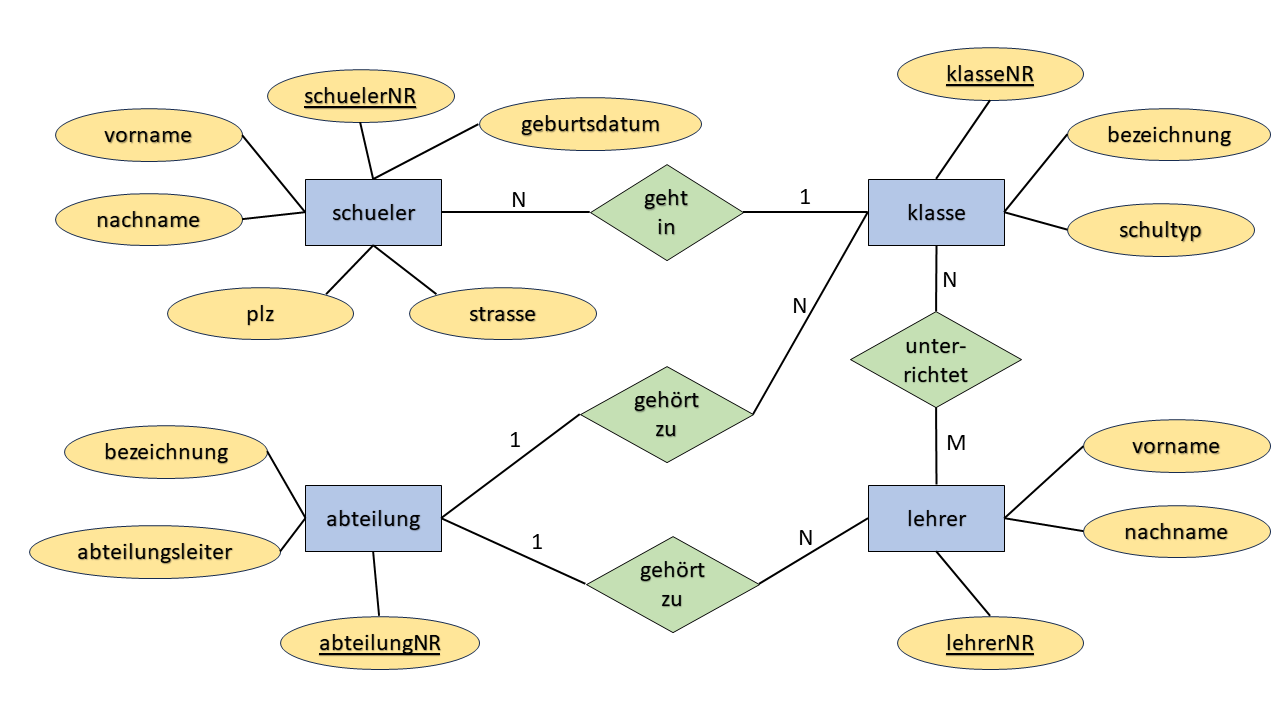
\includegraphics[width=\linewidth]{\pics/schuleDB.png}
		\item Wie viele verschiedene Lehrer unterrichten an der Schule?

		\lstinline!SELECT COUNT(lehrerNR) FROM lehrer;!

		Es sind 17 Lehrer.
		\item Wie viele Schüler kommen aus einer Stadt, deren PLZ mit einer 7 beginnt?

		\lstinline!SELECT COUNT(schuelerNR) FROM schueler WHERE plz between 70000 AND 79999;!

		Es sind 142 Schüler.
		\item Wie viele Lehrer sind den einzelnen Abteilungen jeweils zugeordnet?

		\lstinline[breaklines=true]!SELECT abteilungNR, COUNT(lehrerNR) FROM lehrer_abteilung GROUP BY abteilungNR;!

		\begin{lstlisting}
			3|6
			6|7
			8|3\end{lstlisting}
		\lstinline!SELECT abteilungNR, bezeichnung FROM abteilung;!\\
		\begin{lstlisting}
			3|WG
			6|Berufskolleg
			8|Berufsschule\end{lstlisting}
		Das bedeutet also, dass im WG 6 Lehrer, im Berufskolleg 7 Lehrer und in der Berufsschule 3 Lehrer unterrichten.
	\end{enumerate}
\end{Answer}
	\newpage
	\cohead{\Large\textbf{JOIN-Statement}}
\subsection[JOIN-Statement]{SQL - Das JOIN-Statement}
Öffne die Datenbank \texttt{schuleOptimiert.db} mit dem Datenbank-Browser oder sqlite3.exe.\\
Die Datenbank beinhaltet die gleichen Informationen wie \texttt{schule.db}, jedoch wurde die Datenbank dahingehend optimiert, dass alle zu-1-Beziehungen keine eigene Beziehungstabelle mehr haben. Dies wird das Erstellen der JOIN-Statements erleichtern.
Bisher haben sich unsere SQL-Abfragen immer auf eine einzelne Tabelle bezogen. Viele Fragen lassen sich damit aber nicht oder nicht zufriedenstellend beantworten, z.B. gibt die Tabelle \lstinline!lehrer! indirekt über die \lstinline!abteilungNR! an, welche Lehrer welcher Abteilung zugeordnet sind. Der Anwender möchte jedoch gerne die Zuordnung der Lehrer-Namen zu den Abteilungsbezeichnungen haben, statt der Zuordnung zur \lstinline!abteilungNR!. Dies kann man mit Hilfe des JOIN-Zusatzes erreichen:
\begin{tcolorbox}[title=JOIN-Statement]
	\lstinline!SELECT tabelle1.attribut1, tabelle2.attribut2, usw. FROM tabelle1!\\
	\lstinline!INNER JOIN tabelle2 ON tabelle1.attributx=tabelle2.attributy, usw.;!
\end{tcolorbox}
Nach dem \lstinline!SELECT! gibt man entweder \lstinline!*! für alle Attribute oder  eine Liste von Attributen an. Neu ist, dass man zwischen den Tabellen unterscheiden muss, z.B. steht \lstinline!lehrer.vorname! für das Attribut \lstinline!vorname! aus der Tabelle \lstinline!lehrer!, während \lstinline!schueler.vorname! für das Attribut \lstinline!vorname! aus der Tabelle \lstinline!schueler! steht.\\
\lstinline!FROM tabelle1 INNER JOIN tabelle2! gibt die beiden Tabellen an, die man verknüpfen will.\\
\lstinline!ON bedingungen! gibt an, welche Zeilen der beiden Tabellen als eine ausgegeben werden sollen.\\
\textcolor{red}{ACHTUNG: Ohne \lstinline!ON bedingungen! wird die Potenzmenge gebildet, d.h. jede Zeile der ersten Tabelle wird jeweils mit jeder Zeile der zweiten Tabelle zu jeweils einer Zeile zusammengefasst und ausgegeben, was bei großen Datenbanken zu langen Bearbeitungszeiten führt.}\\
Beispiel:\\
\lstinline!SELECT vorname, nachname, abteilungNR FROM lehrer;!
Gibt die Zuordnung von Lehrern zu Abteilungen an Hand der \lstinline!abteilungNR! an. Diese Darstellung ist abstrakt. Um die Namen der Lehrer und die Bezeichnungen der Abteilungen zu kennen, müssten wir in einer weiteren Tabellen nachschauen. Mit \lstinline!SELECT abteilungNR, bezeichnung FROM abteilung;! können wir der \lstinline!abteilungNR! die Bezeichnung zuordnen und händisch prüfen, welcher Lehrer in welcher Abteilung ist. Bei großen Datensätzen wird dies schnell mühsam.\\
Stattdessen können wir folgendes JOIN-Statement verwenden:\\
\lstinline!SELECT * FROM lehrer INNER JOIN abteilung!\\
\lstinline!ON lehrer.abteilungNR = abteilung.abteilungNR;!
Gibt jeweils in einer Zeile einen Eintrag aus \lstinline!lehrer! und \lstinline!abteilung! aus, so dass die \lstinline!abteilungNR! von beiden Einträgen übereinstimmen.\\
Das DBMS nimmt also die erste Zeile aus \lstinline!lehrer! in die Hand, liest die \lstinline!abteilungNR! aus und geht dann in die Tabelle \lstinline!abteilung!. Es prüft für jede Zeile aus \lstinline!abteilung!, ob die beiden Nummern gleich sind und falls ja, klebt es die Zeilen aus \lstinline!lehrer! und \lstinline!abteilung! nebeneinander, z.B. lautet eine Zeile des Ergebnisses:\\
\lstinline!5|Olaf|Scholz|3|3|WG|Scholz!\\
Der erste Teil \lstinline!5|Olaf|Scholz|3! stammt aus \lstinline!lehrer! mit den Attributen \lstinline!lehrer.lehrerNR=5!, \lstinline!lehrer.vorname=Olaf!, \lstinline!lehrer.nachname=Scholz! und \lstinline!lehrer.abteilungNR=3!. Der zweite Teil \lstinline!3|WG|Scholz! stammt aus \lstinline!abteilung! mit den Attributen \lstinline!abteilung.abteilungNR=3!, \lstinline!abteilung.bezeichnung=WG! und \lstinline!abteilung.abteilungsleiter=Scholz!. Diese beiden Teile wurden zu einer Zeile zusammengefasst, weil die \lstinline!abteilungNR! bei beiden 3 ist.\\
Übersichtlicher ist es, wenn man sich nur die Informationen ausgeben lässt, die relevant sind:\\
\lstinline!SELECT lehrer.vorname, lehrer.nachname, abteilung.bezeichnung FROM lehrer!\\
\lstinline!INNER JOIN abteilung ON lehrer.abteilungNR = abteilung.abteilungNR;!\\
liefert als erste Zeile \lstinline!Olaf|Scholz|WG!.

\begin{Exercise}[title={Bearbeite folgende Aufgaben}, label=Join]
	\begin{enumerate}
		\item Erzeuge eine Ausgabe, die dem Vor- und Nachnamen der Lehrer jeweils die passenden Abteilungsbezeichnungen zuordnet.
		\item Erzeuge eine Ausgabe, die dem Vor- und Nachnamen aller Schüler jeweils die Bezeichnung der passenden Klasse zuordnet.
		\item Erzeuge eine Ausgabe, die jeder Klassenbezeichnung die Anzahl der Schüler der Klasse zuordnet. Tipp: COUNT-Funktion verwenden.
		\item Erzeuge eine Ausgabe, die dem Vor- und Nachnamen aller Schüler jeweils den passenden Schultyp zuordnet. Tipp: Man muss zwei JOIN-Statements verwenden.
	\end{enumerate}
\end{Exercise}
%%%%%%%%%%%%%%%%%%%%%%%%%%%%%%%%%%%%%%%%%
\begin{Answer}[ref=Join]
	\begin{enumerate}
		\item Erzeuge eine Ausgabe, die dem Vor- und Nachnamen der Lehrer jeweils die passenden Abteilungsbezeichnungen zuordnet.\\
		\lstinline!SELECT lehrer.vorname, lehrer.nachname, abteilung.bezeichnung FROM lehrer INNER JOIN abteilung ON lehrer.abteilungNR = abteilung.abteilungNR;!
		\item Erzeuge eine Ausgabe, die dem Vor- und Nachnamen aller Schüler jeweils die Bezeichnung der passenden Klasse zuordnet.\\
		\lstinline!SELECT schueler.vorname, schueler.nachname, klasse.bezeichnung FROM schueler INNER JOIN klasse ON schueler.klasseNR = klasse.klasseNR;!
		\item Erzeuge eine Ausgabe, die jeder Klassenbezeichnung die Anzahl der Schüler der Klasse zuordnet. Tipp: COUNT-Funktion verwenden.\\
		\lstinline!SELECT klasse.bezeichnung, COUNT(klasse.bezeichnung) FROM schueler INNER JOIN klasse ON schueler.klasseNR = klasse.klasseNR GROUP BY klasse.bezeichnung;!
		\item Erzeuge eine Ausgabe, die dem Vor- und Nachnamen aller Schüler jeweils den passenden Schultyp zuordnet. Tipp: Man muss zwei JOIN-Statements verwenden.\\
		\lstinline!SELECT schueler.vorname, schueler.nachname, abteilung.bezeichnung FROM schueler INNER JOIN klasse ON schueler.klasseNR = klasse.klasseNR INNER JOIN abteilung ON klasse.abteilungNR = abteilung.abteilungNR;!
	\end{enumerate}
\end{Answer}
    \newpage
    \cohead{\Large\textbf{Lösungen}}
    \rohead{Lösungen}
    \section{Lösungen der Aufgaben}
    \shipoutAnswer
%    \newpage
%    \cohead{\Large\textbf{Anhang}}
%    \rohead{Anhang}
%    \section{Anhang: Im Skript verwendete Datenbanken}
%    % !TeX root = ../Skript_DB.tex
\cohead{\Large\textbf{Datenbanken}}
\subsection[verwendete Datenbanken]{verwendete Datenbanken}
Die für die Übungsaufgaben verwendeten Datenbanken sind
\begin{itemize}
	\item \lstinline!vieleSchueler.db! für die Kapitel \nameref{select},  \nameref{where}, \nameref{delete} und \nameref{update}
	\item \lstinline!schule.db! für das Kapitel \nameref{funktionen}
	\item \lstinline!schuleOptimiert.db! für das Kapitel \nameref{join}
\end{itemize}
\textcolor{red}{Die verwendeten Datenbanken finden sich auch unter
    {\small\href{https://github.com/hoerm007/DatenbankenSkript\_KaufmBK\_BW/tree/main/Datenbanken}{https://github.com/hoerm007/DatenbankenSkript\_KaufmBK\_BW/tree/main/Datenbanken}}}
\subsubsection{\lstinline!vieleSchueler.db!}
\begin{lstlisting}[breaklines=True, numbers=none, basicstyle=\tiny, keepspaces=false]
	CREATE TABLE schueler(schuelerNR INT PRIMARY KEY NOT NULL, vorname TEXT, nachname TEXT, plz INT, geburtsdatum TEXT, klasse TEXT);
	INSERT INTO schueler VALUES(1,'Anica','Nosudohein',6268,'06.11.1998','BKFH');
	INSERT INTO schueler VALUES(2,'Marlies','Gavofu',25361,'06.01.2002','BK2');
	INSERT INTO schueler VALUES(3,'Franz','Rotagateson',71296,'13.01.1998','BK1');
	INSERT INTO schueler VALUES(4,'Elisabeth','Kotibodoweiner',14798,'20.11.2003','BK1');
	INSERT INTO schueler VALUES(5,'Henni','Kitavare',22926,'21.07.1999','BK2');
	INSERT INTO schueler VALUES(6,'Mariana','Hewalode',23879,'19.05.2004','BK2');
	INSERT INTO schueler VALUES(7,'Henry','Zütuschatthein',94405,'31.12.2004','BK1');
	INSERT INTO schueler VALUES(8,'Fatma','Varobason',19370,'08.01.2005','BK1');
	INSERT INTO schueler VALUES(9,'Gundel','Culufledemeiner',97896,'12.04.1996','BKFH');
	INSERT INTO schueler VALUES(10,'Reinhold','Tulimattson',25821,'08.08.1997','BK1');
	INSERT INTO schueler VALUES(11,'Silvia','Cüwiwattemüller',88339,'09.11.2001','BK2');
	INSERT INTO schueler VALUES(12,'Wiltrud','Dewubaweiner',97980,'','BK2');
	INSERT INTO schueler VALUES(13,'Stefania','Maier',46499,'15.05.1997','BK2');
	INSERT INTO schueler VALUES(14,'Luzia','Sasuwadeson',39397,'17.01.2005','BKFH');
	INSERT INTO schueler VALUES(15,'Sabine','Lelafaremüller',94405,'09.02.1999','BKFH');
	INSERT INTO schueler VALUES(16,'Janine','Teliflede',95659,'11.01.2001','BKFH');
	INSERT INTO schueler VALUES(17,'Jo','Butodoson',2894,'14.03.2006','BK2');
	INSERT INTO schueler VALUES(18,'Hubertus','Palibodoson',97769,'06.11.2004','BK2');
	INSERT INTO schueler VALUES(19,'Patrik','Pöwisedehein',32469,'05.11.2001','BKFH');
	INSERT INTO schueler VALUES(20,'Leopold','Neumann',75433,'','BK1');
	INSERT INTO schueler VALUES(21,'Victoria','Mayer',86807,'01.05.2004','BK1');
	INSERT INTO schueler VALUES(22,'Stanislaw','Suvilodeweiner',6242,'10.01.1997','');
	INSERT INTO schueler VALUES(23,'Anneli','Fasohede',3205,'24.10.2004','BK2');
	INSERT INTO schueler VALUES(24,'Francisco','Nuvuhedemeiner',79400,'02.07.2003','BKFH');
	INSERT INTO schueler VALUES(25,'Reinhild','Wolf',32839,'20.12.2006','BKFH');
	INSERT INTO schueler VALUES(26,'Diether','Jotesadeweiner',9376,'16.07.1998','BKFH');
	INSERT INTO schueler VALUES(27,'Czeslaw','Südefuweiner',7580,'14.09.2002','BK1');
	INSERT INTO schueler VALUES(28,'Betti','Fiwihedemüller',84489,'30.06.2001','BK1');
	INSERT INTO schueler VALUES(29,'Kamil','Dävibiweiner',4655,'11.02.2005','BKFH');
	INSERT INTO schueler VALUES(30,'Irmengard','Kuvegedemüller',44787,'11.05.1996','BK2');
	INSERT INTO schueler VALUES(31,'Samira','Posisadehein',74731,'07.05.1995','BK2');
	INSERT INTO schueler VALUES(32,'Walther','Wowedumüller',63897,'10.12.2001','BKFH');
	INSERT INTO schueler VALUES(33,'Philomena','Jerofoweiner',63897,'','');
	INSERT INTO schueler VALUES(34,'Brigitta','Schmidt',97215,'08.09.2003','BKFH');
	INSERT INTO schueler VALUES(35,'Czeslaw','Tarugaumeiner',14641,'27.05.2002','BK1');
	INSERT INTO schueler VALUES(36,'Katja','Dalavode',6537,'11.01.1995','BK2');
	INSERT INTO schueler VALUES(37,'Florian','Kidulau',73441,'10.11.1996','BK2');
	INSERT INTO schueler VALUES(38,'Veronika','Coramode',73235,'18.12.2000','BKFH');
	INSERT INTO schueler VALUES(39,'Gabi','Zitofaremüller',63619,'12.03.1999','BK1');
	INSERT INTO schueler VALUES(40,'Karla','Lurubedemüller',91083,'24.07.2006','BK2');
	INSERT INTO schueler VALUES(41,'Karl-Werner','Torubuweiner',24321,'04.02.1995','');
	INSERT INTO schueler VALUES(42,'Wilma','Vutagate',26419,'07.03.2003','BKFH');
	INSERT INTO schueler VALUES(43,'Therese','Cedimatt',59348,'09.01.1997','BKFH');
	INSERT INTO schueler VALUES(44,'Theodoros','Jüwavadeson',27283,'09.07.2000','BK1');
	INSERT INTO schueler VALUES(45,'Burghard','Wetogatemüller',9557,'14.01.1998','BK2');
	INSERT INTO schueler VALUES(46,'Giovanna','Dädasege',72275,'03.03.1999','BKFH');
	INSERT INTO schueler VALUES(47,'Gerti','Pilabestein',38820,'29.10.2000','BKFH');
	INSERT INTO schueler VALUES(48,'Dörte','Püdifuhein',77723,'28.09.1998','BK2');
	INSERT INTO schueler VALUES(49,'Gunter','Zäwowattehein',18334,'20.05.2001','BKFH');
	INSERT INTO schueler VALUES(50,'Walentina','Sölibodomeiner',56743,'27.03.1997','BK2');
	INSERT INTO schueler VALUES(51,'Damaris','Mayer',65439,'15.07.2003','BKFH');
	INSERT INTO schueler VALUES(52,'Lina','Hartmann',66386,'10.06.1999','BK2');
	INSERT INTO schueler VALUES(53,'Patricia','Zavusade',19243,'08.01.2000','BKFH');
	INSERT INTO schueler VALUES(54,'Reimer','Bowusadeweiner',56766,'04.10.2006','BK2');
	INSERT INTO schueler VALUES(55,'Annelene','Sedilodeweiner',NULL,'27.11.2006','BK2');
	INSERT INTO schueler VALUES(56,'Ayten','Vatigateweiner',3130,'','BK2');
	INSERT INTO schueler VALUES(57,'Lorenz','Gorobe',73430,'01.04.1999','BK1');
	INSERT INTO schueler VALUES(58,'Annegrete','Cosogaustein',89542,'26.12.2002','BK2');
	INSERT INTO schueler VALUES(59,'Anita','Darusedeweiner',76870,'29.12.2003','BKFH');
	INSERT INTO schueler VALUES(60,'Ercan','Dülofare',79346,'17.09.1995','BK1');
	INSERT INTO schueler VALUES(61,'Hartwig','Jöwebahein',97769,'08.03.1996','BK1');
	INSERT INTO schueler VALUES(62,'Benedikt','Fevesegeweiner',91567,'07.08.1998','BKFH');
	INSERT INTO schueler VALUES(63,'Albina','Boribuhein',6642,'28.02.2007','BKFH');
	INSERT INTO schueler VALUES(64,'Horst-Peter','Javovade',74245,'29.10.1996','BK2');
	INSERT INTO schueler VALUES(65,'Hermann','Zusofu',15749,'28.06.2005','BK1');
	INSERT INTO schueler VALUES(66,'Magda','Mutifomüller',19399,'19.03.2006','BK1');
	INSERT INTO schueler VALUES(67,'Walburga','Fedugate',4838,'27.05.1997','BK1');
	INSERT INTO schueler VALUES(68,'Heinz-Günther','Sivusadeson',88161,'14.09.2001','BK1');
	INSERT INTO schueler VALUES(69,'Fredy','Wäwifomeiner',57518,'09.05.2000','BK1');
	INSERT INTO schueler VALUES(70,'Mato','Reledi',38667,'30.06.2003','BK2');
	INSERT INTO schueler VALUES(71,'Marlies','Schmidt',56203,'11.06.1998','BK2');
	INSERT INTO schueler VALUES(72,'Sinaida','Dasowadestein',94405,'12.03.1999','BK2');
	INSERT INTO schueler VALUES(73,'Anka','Hawasade',93149,'31.03.2003','BK2');
	INSERT INTO schueler VALUES(74,'Tomas','Gulogradehein',15537,'02.12.2003','BK1');
	INSERT INTO schueler VALUES(75,'Hans-Günther','Kotovadestein',50667,'26.07.2001','BK1');
	INSERT INTO schueler VALUES(76,'Florentine','Däragatehein',35410,'10.07.1998','BKFH');
	INSERT INTO schueler VALUES(77,'Anna-Luise','Schulze',23758,'03.07.1998','BKFH');
	INSERT INTO schueler VALUES(78,'Waldtraut','Vurasegemeiner',61130,'16.04.2003','BKFH');
	INSERT INTO schueler VALUES(79,'Otmar','Hesefareson',19406,'18.02.2002','BKFH');
	INSERT INTO schueler VALUES(80,'Dragan','Jösumauhein',8258,'','BKFH');
	INSERT INTO schueler VALUES(81,'Robin','Nüvofimüller',75417,'15.06.2003','BKFH');
	INSERT INTO schueler VALUES(82,'Francesco','Lüriflodemeiner',8118,'29.08.2004','BK1');
	INSERT INTO schueler VALUES(83,'Inga','Zärabahein',32825,'08.07.2002','BK2');
	INSERT INTO schueler VALUES(84,'Malte','Gesabedemeiner',55566,'17.10.2005','BK2');
	INSERT INTO schueler VALUES(85,'Gereon','Lange',7937,'16.06.2004','BKFH');
	INSERT INTO schueler VALUES(86,'Domenico','Zötesegemeiner',71739,'30.08.1997','BKFH');
	INSERT INTO schueler VALUES(87,'Vera','Borumattweiner',47051,'01.04.1995','BK1');
	INSERT INTO schueler VALUES(88,'Aloys','Kotubameiner',23769,'10.08.2003','BK1');
	INSERT INTO schueler VALUES(89,'Joana','Herrmann',89257,'04.07.2002','BK1');
	INSERT INTO schueler VALUES(90,'Gönül','Fawuvadehein',6484,'18.07.2005','');
	INSERT INTO schueler VALUES(91,'Pascale','Rutagate',6895,'26.07.1995','BKFH');
	INSERT INTO schueler VALUES(92,'Veit','Schmid',35423,'03.02.1996','BK1');
	INSERT INTO schueler VALUES(93,'Adam','Gavisadeson',37083,'25.12.2003','BKFH');
	INSERT INTO schueler VALUES(94,'Priska','Fusifiweiner',53572,'30.05.1998','BKFH');
	INSERT INTO schueler VALUES(95,'Irmingard','Nödidu',78098,'24.08.2000','BKFH');
	INSERT INTO schueler VALUES(96,'Carsten','Kätahedestein',52222,'27.02.1995','BKFH');
	INSERT INTO schueler VALUES(97,'Walfried','Jutulau',67697,'05.03.2001','BK2');
	INSERT INTO schueler VALUES(98,'Karl-Ludwig','Cuvibiweiner',50321,'05.04.2003','BK1');
	INSERT INTO schueler VALUES(99,'Cornelius','Neumann',58791,'04.03.2007','BK2');
	INSERT INTO schueler VALUES(100,'Lisette','Kadedumüller',19417,'10.07.1997','BKFH');
\end{lstlisting}
\subsubsection{\lstinline!schule.db!}
\begin{lstlisting}[breaklines=True, numbers=none, basicstyle=\tiny, keepspaces=false]
	CREATE TABLE schueler(schuelerNR INT PRIMARY KEY NOT NULL,nachname TEXT,vorname TEXT,strasse TEXT,plz INT,geburtsdatum TEXT);
	INSERT INTO schueler VALUES(1587,'Muteplau','Tilly','Schulstrasse 110d',65549,'10.06.2005');
	INSERT INTO schueler VALUES(4293,'Jatuhedestein','Rupert','Teichstrasse 272',65549,'08.02.2005');
	INSERT INTO schueler VALUES(114,'Gewubedeweiner','Nuray','Weiherstrasse 236',65582,'08.09.2003');
	INSERT INTO schueler VALUES(1236,'Vevefimeiner','Heinz','Kirchplatz 273',65582,'21.12.2005');
	INSERT INTO schueler VALUES(2468,'Dodusede','Heinz-Georg','Rosenstrasse 9',65582,'06.09.2006');
	INSERT INTO schueler VALUES(3530,'Vutugedemeiner','Andre','Marienstrasse 14',65582,'21.09.2003');
	INSERT INTO schueler VALUES(3976,'Meier','Ottomar','Heckenweg 205',65582,'08.09.1995');
	INSERT INTO schueler VALUES(747,'Mosagatestein','Romuald','Buchenweg 76',65589,'06.06.2001');
	INSERT INTO schueler VALUES(3403,'Törofumüller','Achim','Fichtenstrasse 98',65594,'16.12.1995');
	INSERT INTO schueler VALUES(2680,'Howabeweiner','Meinhard','Finkenstrasse 105',65719,'24.04.1995');
	INSERT INTO schueler VALUES(2964,'Tuloschattweiner','Ramon','Veilchenweg 47',65719,'07.08.1998');
	INSERT INTO schueler VALUES(3781,'Juwoplauweiner','Hannes','Südstrasse 139',65719,'13.07.1998');
	INSERT INTO schueler VALUES(3956,'Gutovorehein','Siegfried','Waldweg 258',65760,'03.12.2003');
	INSERT INTO schueler VALUES(1232,'Falevare','Rosi','Schubertstrasse 264',65779,'18.11.1998');
	INSERT INTO schueler VALUES(1481,'Lehmann','Gesche','Siemensstrasse 182',65779,'03.12.1998');
	INSERT INTO schueler VALUES(3810,'Rötoda','Mareike','Veilchenweg 68',65779,'06.04.1996');
	INSERT INTO schueler VALUES(1170,'Schäfer','Gesa','Buchenweg 169',65795,'30.10.2004');
	INSERT INTO schueler VALUES(3204,'Huber','Caren','Burgstrasse 93',65812,'11.02.2006');
	INSERT INTO schueler VALUES(457,'Jotavoremeiner','Wiltrud','Hohe Strasse 135',65817,'27.04.2001');
	INSERT INTO schueler VALUES(2763,'Mülimaumeiner','Aleksandra','Feldstrasse 121',65824,'18.03.1997');
	INSERT INTO schueler VALUES(4848,'Fotovaremüller','Suzanne','Holunderweg 188',65824,'05.12.2006');
	INSERT INTO schueler VALUES(746,'Nevebodostein','Esther','Mittelstrasse 46',66111,'28.07.1999');
	INSERT INTO schueler VALUES(1811,'Dutafumeiner','Cilli','Steinstrasse 136',66111,'04.08.1995');
	INSERT INTO schueler VALUES(1936,'Jowemattstein','Irmtraut','Max-Planck-Strasse 117',66280,'15.06.1999');
	INSERT INTO schueler VALUES(2246,'Havufu','Yasemin','August-Bebel-Strasse 152',66280,'30.06.2004');
	INSERT INTO schueler VALUES(4945,'Sewisademeiner','Frieda','Kantstrasse 210',66280,'18.03.2004');
	INSERT INTO schueler VALUES(772,'Fotulaustein','Hasan','Querstrasse 247',66299,'11.06.2000');
	INSERT INTO schueler VALUES(2844,'Golusege','Krista','Kolpingstrasse 88',66299,'24.01.2005');
	INSERT INTO schueler VALUES(3391,'Mürudason','Cosima','Ahornstrasse 225',66299,'20.02.2001');
	INSERT INTO schueler VALUES(3946,'Lehmann','Valeska','Im Wiesengrund 174',66299,'07.08.2000');
	INSERT INTO schueler VALUES(2744,'Turolatehein','Renato','Steinstrasse 14',66333,'11.01.1996');
	INSERT INTO schueler VALUES(2976,'Weber','Hans-Peter','Schlehenweg 103',66333,'22.10.1996');
	INSERT INTO schueler VALUES(2255,'Givedimeiner','Carl-Heinz','Am Friedhof 99',66346,'22.11.2004');
	INSERT INTO schueler VALUES(52,'Hartmann','Lina','Eichenstrasse 78',66386,'20.06.1995');
	INSERT INTO schueler VALUES(1449,'Tetaschattmüller','Timo','Mühlstrasse 132',66386,'12.04.2005');
	INSERT INTO schueler VALUES(3021,'Tilolaumüller','Karen','Starenweg 230',66386,'04.10.2001');
	INSERT INTO schueler VALUES(3603,'Vuraflede','Sibel','Lerchenstrasse 234',66386,'02.10.2000');
	INSERT INTO schueler VALUES(849,'Vosibodoweiner','Cemal','Gutenbergstrasse 72',66424,'16.03.2001');
	INSERT INTO schueler VALUES(2553,'Neumann','Kristian','Starenweg 244',66424,'04.12.2004');
	INSERT INTO schueler VALUES(2140,'Züvasedeson','Eugenia','Schubertstrasse 137',66440,'12.03.1996');
	INSERT INTO schueler VALUES(408,'Betoschattmüller','Danilo','Südstrasse 158',66450,'14.08.2000');
	INSERT INTO schueler VALUES(1204,'Walter','Lorenzo','Dieselstrasse 168',66450,'08.12.1999');
	INSERT INTO schueler VALUES(1414,'Meyer','Antonino','Birkenweg 141',66450,'13.11.2003');
	INSERT INTO schueler VALUES(2802,'Werner','Philomena','Fliederweg 88',66482,'04.10.1999');
	INSERT INTO schueler VALUES(104,'Tulaflodeson','Helma','Fichtenweg 191',66500,'07.05.2002');
	INSERT INTO schueler VALUES(194,'Holesege','Marvin','Amselweg 82c',66500,'08.05.2001');
	INSERT INTO schueler VALUES(1556,'Bevelatehein','Rosa-Maria','Mittelweg 219',66500,'12.01.2005');
	INSERT INTO schueler VALUES(3997,'Cäsahedemeiner','Solveig','Im Wiesengrund 79',66500,'12.05.1998');
	INSERT INTO schueler VALUES(4913,'Meier','Hans-Günther','Kirchgasse 296',66500,'04.10.1995');
	INSERT INTO schueler VALUES(328,'Püteferemeiner','Sedat','Kreuzweg 186',66538,'18.03.1997');
	INSERT INTO schueler VALUES(3796,'Haliwatteweiner','Giuseppina','Frühlingstrasse 294',66538,'03.05.2006');
	INSERT INTO schueler VALUES(4350,'Hüribe','Slobodan','Kirchenweg 187',66538,'15.02.1995');
	INSERT INTO schueler VALUES(2866,'Cuwawattemeiner','Elma','Kiefernweg 193d',66564,'03.03.1997');
	INSERT INTO schueler VALUES(4410,'Gutogrodeson','Dragan','Wacholderweg 253',66564,'04.07.1998');
	INSERT INTO schueler VALUES(1209,'Gologrodeweiner','Nikola','Schubertstrasse 228',66606,'25.05.2004');
	INSERT INTO schueler VALUES(1265,'König','Veronica','Gerhart-Hauptmann-Strasse 15',66606,'26.10.2002');
	INSERT INTO schueler VALUES(2606,'Lüvematthein','Rudolph','Lindenallee 88b',66606,'19.05.1996');
	INSERT INTO schueler VALUES(4386,'Tälube','Maria-Luise','Am Anger 253',66606,'31.03.2002');
	INSERT INTO schueler VALUES(3041,'Völufuweiner','Hans-Friedrich','Birkenweg 260',66663,'26.09.2004');
	INSERT INTO schueler VALUES(4792,'Herrmann','Anne','Kreuzstrasse 133',66663,'14.12.2001');
	INSERT INTO schueler VALUES(4338,'Meier','Margaretha','Amselweg 112',66687,'05.02.1996');
	INSERT INTO schueler VALUES(4922,'Bütowattestein','Danuta','Wiesengrund 77',66687,'30.01.1997');
	INSERT INTO schueler VALUES(4806,'Sülavodemüller','Karl-August','Grüner Weg 175',66740,'02.01.1998');
	INSERT INTO schueler VALUES(2045,'Mätuvode','Marjan','Wiesengrund 213',66763,'17.12.1996');
	INSERT INTO schueler VALUES(2344,'König','Wolf','Finkenweg 34',66763,'30.01.2006');
	INSERT INTO schueler VALUES(2839,'Pulafuson','Ian','Pfarrgasse 160',66763,'22.05.2000');
	INSERT INTO schueler VALUES(3633,'Kediflodeweiner','Florian','Kurze Strasse 214',66822,'28.09.1998');
	INSERT INTO schueler VALUES(4359,'Mosodimüller','Nuran','Fasanenweg 275',66822,'27.05.1999');
	INSERT INTO schueler VALUES(1207,'Ridadi','Nikolai','Eichenweg 297',66849,'14.04.2001');
	INSERT INTO schueler VALUES(498,'Meier','Christl','Am Bahnhof 185',66869,'22.06.2006');
	INSERT INTO schueler VALUES(1413,'Huber','Stefano','Dahlienweg 81',66869,'18.04.2005');
	INSERT INTO schueler VALUES(1883,'Kurofu','Rosa','Brunnenweg 143',66869,'02.02.1995');
	INSERT INTO schueler VALUES(2444,'Basobodo','Amir','Veilchenweg 61',66869,'14.01.2001');
	INSERT INTO schueler VALUES(4660,'Jitowatte','Benjamin','Eichenstrasse 208',66869,'10.11.2001');
	INSERT INTO schueler VALUES(4209,'Potifarestein','Viktoria','Jahnstrasse 204',66877,'06.07.2003');
	INSERT INTO schueler VALUES(739,'Dovusegemeiner','Janusz','Industriestrasse 155',66953,'24.03.2002');
	INSERT INTO schueler VALUES(1068,'Verosade','Severin','Luisenstrasse 75',66953,'01.05.2006');
	INSERT INTO schueler VALUES(2211,'Visabodohein','Josephine','Kurze Strasse 174',66953,'10.05.2005');
	INSERT INTO schueler VALUES(2919,'Bitogatestein','Julius','Mühlgasse 264',66953,'29.07.1997');
	INSERT INTO schueler VALUES(2754,'Täwidistein','Elzbieta','Rosenweg 38',66976,'15.03.1996');
	INSERT INTO schueler VALUES(4444,'Leluferestein','Roswita','Wiesenstrasse 95',66976,'28.02.2004');
	INSERT INTO schueler VALUES(4498,'Mayer','Reiner','Weiherstrasse 291',66976,'19.12.2006');
	INSERT INTO schueler VALUES(2060,'Köhler','Mechtild','Schulweg 152',66994,'21.02.2004');
	INSERT INTO schueler VALUES(507,'Purusadeson','Marianne','Tulpenweg 265',67059,'05.03.1997');
	INSERT INTO schueler VALUES(1089,'Bivadu','Darko','Friedensstrasse 134',67059,'25.01.1997');
	INSERT INTO schueler VALUES(1432,'Folufarestein','Mehmet','Kapellenstrasse 63',67059,'27.07.1998');
	INSERT INTO schueler VALUES(4033,'Walter','Caren','Drosselweg 41b',67059,'28.09.2002');
	INSERT INTO schueler VALUES(673,'Teseba','Theres','Haydnstrasse 227a',67098,'20.10.1997');
	INSERT INTO schueler VALUES(1352,'Richter','Horst-Günter','Rathausstrasse 111',67098,'18.07.2004');
	INSERT INTO schueler VALUES(3023,'Hörifimüller','Istvan','Friedrichstrasse 20',67098,'26.08.1995');
	INSERT INTO schueler VALUES(1585,'Belamodemüller','Danuta','Beethovenstrasse 99',67146,'16.10.2004');
	INSERT INTO schueler VALUES(3103,'Rülidostein','Ole','Birkenweg 286b',67157,'13.09.2001');
	INSERT INTO schueler VALUES(3554,'Guwusede','Traude','Lärchenweg 206',67157,'22.05.2006');
	INSERT INTO schueler VALUES(4830,'Zasugate','Nils','Bergstrasse 293',67157,'01.07.1998');
	INSERT INTO schueler VALUES(1041,'Schröder','Wolfgang','Weidenweg 165',67227,'03.01.2001');
	INSERT INTO schueler VALUES(3936,'Detiplau','Nurten','Poststrasse 241',67227,'25.10.1995');
	INSERT INTO schueler VALUES(4385,'Silibehein','Mario','Querstrasse 155',67227,'22.09.1997');
	INSERT INTO schueler VALUES(2373,'Nosolodemüller','Delia','Holunderweg 46',67269,'13.06.2004');
	INSERT INTO schueler VALUES(151,'Lange','Riza','Breslauer Strasse 129',67292,'25.05.2001');
	INSERT INTO schueler VALUES(683,'Sütimatt','Hans-Helmut','Kirchplatz 158',67292,'09.10.1998');
	INSERT INTO schueler VALUES(3645,'Milibemüller','Friedhold','Weinbergstrasse 179',67292,'02.05.1995');
	INSERT INTO schueler VALUES(2893,'Petumau','Editha','Waldstrasse 131',67304,'12.08.2002');
	INSERT INTO schueler VALUES(915,'Taradomüller','Marlen','Ahornstrasse 136',67346,'08.04.1999');
	INSERT INTO schueler VALUES(2979,'Nolusege','Antonius','Waldstrasse 158',67346,'25.08.2004');
	INSERT INTO schueler VALUES(2591,'Sörubimüller','Käte','Industriestrasse 267',67466,'31.08.1999');
	INSERT INTO schueler VALUES(4219,'Tolobistein','Danny','Mühlstrasse 57',67466,'25.08.1995');
	INSERT INTO schueler VALUES(4738,'Rirufihein','Amalie','Robert-Bosch-Strasse 35',67466,'06.11.1997');
	INSERT INTO schueler VALUES(2210,'Viwidumüller','Dana','Rosenstrasse 107',67480,'31.05.2006');
	INSERT INTO schueler VALUES(2960,'Pasewatteson','Hans-Martin','Talstrasse 259',67480,'01.12.1995');
	INSERT INTO schueler VALUES(4482,'Piwasademeiner','Heinfried','Goethestrasse 77',67480,'26.10.2000');
	INSERT INTO schueler VALUES(154,'Hofmann','Wolfgang','Birkenweg 239',67547,'28.01.1995');
	INSERT INTO schueler VALUES(524,'Koch','Ludmila','Schulstrasse 203',67547,'20.09.2006');
	INSERT INTO schueler VALUES(1777,'Rutabu','Lieselotte','Wiesengrund 173',67547,'07.05.2002');
	INSERT INTO schueler VALUES(3222,'Pisalodeson','Karlfried','Danziger Strasse 205',67547,'04.03.2006');
	INSERT INTO schueler VALUES(3397,'Huber','Corinne','Flurstrasse 48',67547,'28.05.2005');
	INSERT INTO schueler VALUES(225,'Hataplaumüller','Helene','Birkenstrasse 196',67574,'26.11.2002');
	INSERT INTO schueler VALUES(2440,'Tulufi','Danielle','Kirchweg 290',67574,'03.04.2005');
	INSERT INTO schueler VALUES(3503,'Cöwubemüller','Agatha','Forststrasse 147',67574,'11.02.2005');
	INSERT INTO schueler VALUES(648,'Cesafuweiner','Silke','Richard-Wagner-Strasse 96',67657,'08.08.2002');
	INSERT INTO schueler VALUES(1199,'Judewademüller','Severin','Mühlweg 117',67657,'09.06.1997');
	INSERT INTO schueler VALUES(97,'Jutulau','Walfried','Karlstrasse 183',67697,'26.05.1999');
	INSERT INTO schueler VALUES(1495,'Schulz','Freddy','Forststrasse 4',67697,'10.05.1995');
	INSERT INTO schueler VALUES(4119,'Hoffmann','Werner','Im Winkel 141',67697,'06.05.1997');
	INSERT INTO schueler VALUES(3259,'Nudimodemeiner','Rolf-Dieter','Parkstrasse 253',67742,'06.06.2001');
	INSERT INTO schueler VALUES(549,'Fischer','Dimitri','Blumenweg 167c',67752,'20.02.1997');
	INSERT INTO schueler VALUES(4262,'Meveba','Valeria','Alte Dorfstrasse 42',67752,'26.10.2003');
	INSERT INTO schueler VALUES(741,'Zadowademüller','Hans','Kastanienweg 255',67806,'19.03.2006');
	INSERT INTO schueler VALUES(1550,'Jiwofoweiner','David','Kreuzstrasse 197',67806,'02.08.1997');
	INSERT INTO schueler VALUES(385,'Cavugedeweiner','Radmila','Tulpenstrasse 188',68519,'20.09.2001');
	INSERT INTO schueler VALUES(927,'Dowugedemeiner','Corina','Uhlandstrasse 75',68519,'04.09.2004');
	INSERT INTO schueler VALUES(4248,'Kasefistein','Mechtild','Albert-Schweitzer-Strasse 281',68519,'20.01.2003');
	INSERT INTO schueler VALUES(997,'Zutedihein','Annelore','Schwarzer Weg 262',68526,'27.02.1995');
	INSERT INTO schueler VALUES(2615,'Wärugatestein','Ralf-Dieter','Schwarzer Weg 271',68526,'06.06.2005');
	INSERT INTO schueler VALUES(4867,'Laradimeiner','Friedrich','Frankenstrasse 245',68526,'04.03.1995');
	INSERT INTO schueler VALUES(1877,'Savifi','Marian','Gerhart-Hauptmann-Strasse 200',68623,'04.02.2003');
	INSERT INTO schueler VALUES(426,'Vuwifistein','Stephanie','Nelkenweg 117',68642,'26.01.1999');
	INSERT INTO schueler VALUES(1263,'Katefuhein','Ingeborg','Grabenstrasse 43',68642,'25.07.1995');
	INSERT INTO schueler VALUES(140,'Sösubameiner','Henriette','Kastanienweg 295c',68723,'28.02.2006');
	INSERT INTO schueler VALUES(1955,'Ritibe','Riza','Gartenweg 61',68753,'07.10.2002');
	INSERT INTO schueler VALUES(409,'Schröder','Klaus-Jürgen','Schulstrasse 91',68766,'12.07.1996');
	INSERT INTO schueler VALUES(2663,'Votuduson','Anne-Marie','Pfarrgasse 224',68766,'12.12.2002');
	INSERT INTO schueler VALUES(3160,'Schmitz','Klaus-Jürgen','Südstrasse 47',68766,'25.01.1999');
	INSERT INTO schueler VALUES(3795,'Nuwufoweiner','Andreas','Ludwigstrasse 101',68766,'07.05.2000');
	INSERT INTO schueler VALUES(341,'Rutufledemüller','Bertram','Hohe Strasse 230',69117,'24.06.2000');
	INSERT INTO schueler VALUES(974,'Jisugatemeiner','Abraham','Fliederweg 150',69117,'04.06.2004');
	INSERT INTO schueler VALUES(2343,'Pävisade','Celal','Grüner Weg 22',69117,'03.12.1998');
	INSERT INTO schueler VALUES(4707,'Fewafuson','Micha','Lessingstrasse 73c',69117,'22.10.2002');
	INSERT INTO schueler VALUES(726,'Cotolatehein','Sigrun','Ahornstrasse 234',69151,'20.06.2000');
	INSERT INTO schueler VALUES(1324,'Husubuweiner','Hanns','Ahornstrasse 215',69151,'14.12.2002');
	INSERT INTO schueler VALUES(1484,'Hasidi','Rosl','Friedhofstrasse 165',69151,'04.11.2006');
	INSERT INTO schueler VALUES(3073,'Fudefu','Aenne','Bahnhofstrasse 48',69151,'22.03.2000');
	INSERT INTO schueler VALUES(3392,'Belagrodemeiner','Gaby','Rotdornweg 18',69151,'09.04.2005');
	INSERT INTO schueler VALUES(907,'Lotabedemeiner','Margret','Querstrasse 240',69168,'15.05.2000');
	INSERT INTO schueler VALUES(1522,'Gütischattmeiner','Tino','Forststrasse 291',69168,'19.01.2003');
	INSERT INTO schueler VALUES(2074,'Fususadehein','Sophie','Kolpingstrasse 74',69168,'28.04.2006');
	INSERT INTO schueler VALUES(4749,'Javivare','Ewald','Falkenweg 57',69168,'24.08.2004');
	INSERT INTO schueler VALUES(3315,'Hevuwadeweiner','Miroslav','Lange Strasse 295',69181,'16.10.2002');
	INSERT INTO schueler VALUES(3361,'Gawesege','Hanspeter','Akazienweg 175',69181,'16.05.2003');
	INSERT INTO schueler VALUES(3081,'Nodefoweiner','Irene','Weidenweg 47',69198,'20.06.1997');
	INSERT INTO schueler VALUES(3649,'Pövibede','Bertram','Starenweg 222',69198,'30.09.2002');
	INSERT INTO schueler VALUES(4334,'Richter','Christiane','Geschwister-Scholl-Strasse 146',69198,'04.02.2000');
	INSERT INTO schueler VALUES(805,'Siwewadehein','Lucie','Geschwister-Scholl-Strasse 244',69214,'20.10.2006');
	INSERT INTO schueler VALUES(2509,'Hiwegatemüller','Roselinde','Heckenweg 76',69231,'19.08.1997');
	INSERT INTO schueler VALUES(4133,'Mutowademeiner','Liane','Sonnenstrasse 30d',69231,'07.06.2000');
	INSERT INTO schueler VALUES(2315,'Hirefihein','Stephanie','Waldstrasse 289',69239,'06.02.2001');
	INSERT INTO schueler VALUES(3665,'Lotesegeson','Jose','Erlenstrasse 63',69239,'21.10.1999');
	INSERT INTO schueler VALUES(1423,'Buramau','Regine','Hohlweg 132',69250,'12.05.2004');
	INSERT INTO schueler VALUES(3663,'Diwuwattestein','Balthasar','Karlstrasse 20',69250,'16.01.2002');
	INSERT INTO schueler VALUES(2443,'Zovobodoweiner','Serpil','Nordstrasse 42',69412,'13.04.2001');
	INSERT INTO schueler VALUES(885,'Fasodo','Etta','Amselweg 259',69434,'12.01.1999');
	INSERT INTO schueler VALUES(2340,'Nerusedestein','Heinz-Dieter','Friedensstrasse 247',69434,'20.09.2001');
	INSERT INTO schueler VALUES(2436,'Häralauweiner','Hanni','Kreuzstrasse 253',69469,'02.11.1999');
	INSERT INTO schueler VALUES(2732,'Lowugradehein','Elena','Kirchplatz 134',69469,'06.05.2006');
	INSERT INTO schueler VALUES(3193,'Bewogate','Marietta','Drosselweg 228',69469,'31.12.1996');
	INSERT INTO schueler VALUES(4984,'Schmidt','Jaroslav','Blumenstrasse 44',69469,'02.01.2003');
	INSERT INTO schueler VALUES(1530,'Vilugrade','Else','Siemensstrasse 53',69502,'11.09.2006');
	INSERT INTO schueler VALUES(1764,'Gitaflodehein','Erhardt','Friedensstrasse 206',69502,'08.04.2000');
	INSERT INTO schueler VALUES(2556,'Lövegrode','Michaele','Frühlingstrasse 83',69502,'03.07.1999');
	INSERT INTO schueler VALUES(736,'Wävuwatte','Manuela','Hochstrasse 32',70173,'22.09.2002');
	INSERT INTO schueler VALUES(886,'Bisuvoreson','Magarete','Karlstrasse 119',70173,'18.11.2004');
	INSERT INTO schueler VALUES(1834,'Hoffmann','Leon','Bahnhofstrasse 197',70173,'10.10.2001');
	INSERT INTO schueler VALUES(4327,'Powofuhein','Sebastiano','Geschwister-Scholl-Strasse 252',70173,'24.09.1996');
	INSERT INTO schueler VALUES(4392,'Hofmann','Ingbert','Raiffeisenstrasse 257',70173,'16.01.1995');
	INSERT INTO schueler VALUES(2209,'Sowumodehein','Hülya','Geschwister-Scholl-Strasse 58',70734,'27.08.2006');
	INSERT INTO schueler VALUES(2570,'Nädivode','Ekkehart','Buchenstrasse 2',70734,'07.12.1999');
	INSERT INTO schueler VALUES(2150,'Koch','Paulina','Fichtenweg 123',70771,'29.10.2002');
	INSERT INTO schueler VALUES(3343,'Wolf','Antonius','Mühlgasse 202',70771,'10.02.2002');
	INSERT INTO schueler VALUES(4657,'Feruwedemüller','Hubert','Birkenweg 57',70771,'12.03.1999');
	INSERT INTO schueler VALUES(1885,'Barovade','Amalia','Hochstrasse 178',70794,'09.07.2001');
	INSERT INTO schueler VALUES(3442,'Dewuvoreson','Heide','Lange Strasse 128',70794,'21.01.2004');
	INSERT INTO schueler VALUES(4471,'Meier','Kevin','Friedenstrasse 95',70794,'31.01.2006');
	INSERT INTO schueler VALUES(1754,'Jovewedehein','Siegmar','Lindenweg 122',70806,'21.12.2002');
	INSERT INTO schueler VALUES(2562,'Dovofarestein','Reiner','Haydnstrasse 181',70806,'23.09.1999');
	INSERT INTO schueler VALUES(4598,'Bidabeson','Meral','Robert-Koch-Strasse 104',70806,'09.04.2005');
	INSERT INTO schueler VALUES(810,'Hudiferestein','Lia','Pappelweg 232',70825,'29.09.2004');
	INSERT INTO schueler VALUES(2087,'Cotisedehein','Gerhard','Schwarzer Weg 103',70825,'03.03.2003');
	INSERT INTO schueler VALUES(2330,'Perolateson','Philip','Jägerstrasse 196',70839,'07.08.1999');
	INSERT INTO schueler VALUES(3095,'Tovifostein','Nelli','Grenzweg 132',70839,'11.08.1997');
	INSERT INTO schueler VALUES(3996,'Ditofarestein','Attila','Kirchstrasse 80',70839,'21.10.2004');
	INSERT INTO schueler VALUES(788,'Kewemodeson','Adriana','Seestrasse 209',71032,'30.12.1996');
	INSERT INTO schueler VALUES(1561,'Werner','Helmtrud','Bismarckstrasse 158',71032,'05.03.2003');
	INSERT INTO schueler VALUES(1625,'Wädaplauson','Ruben','Brunnenstrasse 216',71032,'18.01.2005');
	INSERT INTO schueler VALUES(1843,'Tavilodemüller','Gerolf','Sandweg 99',71032,'13.04.1997');
	INSERT INTO schueler VALUES(2333,'Hoffmann','Rose','Eschenweg 3',71032,'21.09.1998');
	INSERT INTO schueler VALUES(3929,'Wolf','Hans-Adolf','Schlehenweg 273',71032,'22.08.1999');
	INSERT INTO schueler VALUES(4203,'König','Senta','Eichenstrasse 12',71032,'24.07.1998');
	INSERT INTO schueler VALUES(4580,'Getevodeweiner','Ludwina','Weinbergstrasse 72b',71032,'28.08.2001');
	INSERT INTO schueler VALUES(2946,'Katagrade','Guido','Kolpingstrasse 289',71083,'04.12.1995');
	INSERT INTO schueler VALUES(4259,'Celofaremüller','Kriemhild','Richard-Wagner-Strasse 14',71083,'17.08.1999');
	INSERT INTO schueler VALUES(178,'Merelode','Gino','Parkstrasse 134b',71088,'17.01.2000');
	INSERT INTO schueler VALUES(3693,'Ruvufuson','Karl-Ernst','Akazienweg 231',71088,'22.09.2003');
	INSERT INTO schueler VALUES(725,'Bivagradeweiner','Diedrich','Falkenweg 104',71111,'14.04.1997');
	INSERT INTO schueler VALUES(1468,'Gusiplau','Natalie','Uhlandstrasse 40',71229,'11.07.2002');
	INSERT INTO schueler VALUES(2554,'Sesoflodemeiner','Sebastian','Gartenstrasse 271',71229,'13.04.1996');
	INSERT INTO schueler VALUES(4043,'Volagau','Michaele','Wiesenstrasse 16b',71229,'21.03.1997');
	INSERT INTO schueler VALUES(108,'Becker','Georgios','Friedhofstrasse 216d',71254,'14.08.1996');
	INSERT INTO schueler VALUES(476,'Dotahedemüller','Domenico','Lärchenweg 235',71254,'19.09.2004');
	INSERT INTO schueler VALUES(3687,'Palolate','Sahin','Breslauer Strasse 193',71254,'29.10.1997');
	INSERT INTO schueler VALUES(4764,'Müdigedemüller','Rupert','Am Hang 158',71254,'18.10.2006');
	INSERT INTO schueler VALUES(368,'Lehmann','Frithjof','Brückenstrasse 291',71272,'25.12.2000');
	INSERT INTO schueler VALUES(1139,'Masusedeweiner','Falko','Heinrich-Heine-Strasse 78',71272,'22.12.1997');
	INSERT INTO schueler VALUES(3916,'Nidugrodehein','Annemarie','Am Friedhof 211b',71272,'10.08.2002');
	INSERT INTO schueler VALUES(123,'Cusovore','Samira','Blumenweg 199',71277,'26.10.1999');
	INSERT INTO schueler VALUES(521,'Zudegrode','Kristiane','Heideweg 176',71277,'28.09.1999');
	INSERT INTO schueler VALUES(3,'Rotagateson','Franz','Weidenweg 209d',71296,'05.10.2002');
	INSERT INTO schueler VALUES(960,'Welifoson','Betina','Tannenweg 119',71296,'19.02.2004');
	INSERT INTO schueler VALUES(2307,'Matigradeson','Ingbert','Nordstrasse 19',71296,'23.02.1998');
	INSERT INTO schueler VALUES(2917,'Schmitt','Ekkehart','Königsberger Strasse 237',71296,'16.12.1996');
	INSERT INTO schueler VALUES(1486,'Rowisademeiner','Melissa','Tulpenstrasse 171',71332,'04.01.2003');
	INSERT INTO schueler VALUES(701,'Jitavade','Berndt','Lilienweg 122',71364,'05.03.1998');
	INSERT INTO schueler VALUES(1426,'Lilafi','Stefano','Ulmenweg 118',71364,'03.01.1995');
	INSERT INTO schueler VALUES(4196,'Dawivodeweiner','Benno','Schillerstrasse 270',71364,'29.05.1999');
	INSERT INTO schueler VALUES(2259,'Müller','Francisco','Fichtenstrasse 42',71384,'26.10.2004');
	INSERT INTO schueler VALUES(1748,'Schmid','Antonino','Burgstrasse 103',71522,'04.12.1997');
	INSERT INTO schueler VALUES(2852,'Hartmann','Telse','Ahornstrasse 2a',71522,'13.09.2001');
	INSERT INTO schueler VALUES(2599,'Zitebeson','Norbert','Lindenweg 279',71540,'19.07.2000');
	INSERT INTO schueler VALUES(3352,'Tisodaweiner','Inge','Gartenweg 180c',71540,'18.06.1995');
	INSERT INTO schueler VALUES(537,'Koch','Jenny','August-Bebel-Strasse 236',71665,'01.10.1996');
	INSERT INTO schueler VALUES(2815,'Jutifomeiner','Luisa','Heinrich-Heine-Strasse 247',71665,'05.09.2002');
	INSERT INTO schueler VALUES(617,'Schmidt','Muharrem','Querstrasse 197',71672,'29.11.1995');
	INSERT INTO schueler VALUES(1755,'Pirewattemüller','Marius','Robert-Koch-Strasse 8',71672,'09.04.2001');
	INSERT INTO schueler VALUES(1923,'Kiremode','Antonina','Kirchweg 240',71672,'03.02.1996');
	INSERT INTO schueler VALUES(2861,'Pudemode','Isabella','Haydnstrasse 166c',71672,'12.12.2003');
	INSERT INTO schueler VALUES(3375,'Katubodoson','Rena','Starenweg 74',71672,'28.10.1997');
	INSERT INTO schueler VALUES(4214,'Vesadostein','Engelbert','Industriestrasse 232',71672,'01.07.2000');
	INSERT INTO schueler VALUES(4351,'Wolf','Igor','Max-Planck-Strasse 238',71672,'02.08.2002');
	INSERT INTO schueler VALUES(4863,'Cosewedemüller','Meik','Grenzweg 297b',71672,'08.09.2004');
	INSERT INTO schueler VALUES(424,'Gövufu','Leopoldine','Heinrich-Heine-Strasse 141',71679,'04.06.2004');
	INSERT INTO schueler VALUES(1514,'Bauer','Adriane','Forststrasse 159',71679,'01.04.2005');
	INSERT INTO schueler VALUES(1586,'Schröder','Hans-Christian','Blumenstrasse 3',71679,'14.05.2005');
	INSERT INTO schueler VALUES(2322,'Horugatemeiner','Moritz','Robert-Koch-Strasse 8',71679,'07.12.1999');
	INSERT INTO schueler VALUES(3255,'Nülivade','Helena','Lilienweg 173',71679,'31.05.2006');
	INSERT INTO schueler VALUES(4756,'Schwarz','Marlis','Kurze Strasse 208a',71679,'21.05.1997');
	INSERT INTO schueler VALUES(1797,'Herrmann','Ann-Kathrin','Mozartstrasse 289',71686,'13.01.1998');
	INSERT INTO schueler VALUES(951,'Schröder','Paulo','Akazienweg 95a',71691,'29.06.2000');
	INSERT INTO schueler VALUES(477,'Zövafare','Reinhard','Friedenstrasse 8',71706,'08.09.1999');
	INSERT INTO schueler VALUES(1871,'Rodawedemeiner','Ole','Lange Strasse 239',71706,'11.06.1998');
	INSERT INTO schueler VALUES(3858,'Gölogrodeson','Reni','Schwalbenweg 262',71706,'28.04.1999');
	INSERT INTO schueler VALUES(4635,'Zöteflode','Benno','Berliner Strasse 199',71706,'19.04.1997');
	INSERT INTO schueler VALUES(1653,'Dasofarehein','Romana','Schwarzer Weg 248',71711,'31.07.2003');
	INSERT INTO schueler VALUES(3302,'Schmid','Hansjürgen','Weinbergstrasse 213',71711,'25.05.2005');
	INSERT INTO schueler VALUES(2335,'Heluflede','Annett','Mörikestrasse 49',71717,'23.01.1995');
	INSERT INTO schueler VALUES(3608,'Vureduhein','Sepp','Schubertstrasse 161',71717,'13.03.1999');
	INSERT INTO schueler VALUES(755,'Hewebehein','Artur','Tulpenweg 12',71723,'28.06.2003');
	INSERT INTO schueler VALUES(86,'Zötesegemeiner','Domenico','Grabenstrasse 297',71739,'20.06.2005');
	INSERT INTO schueler VALUES(3469,'Zatuplauson','Eric','Nelkenweg 298',71739,'11.06.1997');
	INSERT INTO schueler VALUES(3657,'Patodumeiner','Antonie','Goethestrasse 298b',71739,'03.06.2005');
	INSERT INTO schueler VALUES(703,'Kotovodemeiner','Vesna','Robert-Bosch-Strasse 129',72070,'03.12.1995');
	INSERT INTO schueler VALUES(2359,'Watemaustein','Eckhardt','Brückenstrasse 75',72070,'14.02.1999');
	INSERT INTO schueler VALUES(3307,'Lolofaremeiner','Theresia','Robert-Bosch-Strasse 7',72070,'09.09.2005');
	INSERT INTO schueler VALUES(4117,'Hituvademeiner','Thekla','Wilhelmstrasse 92b',72070,'28.08.2006');
	INSERT INTO schueler VALUES(1309,'Ridiwedehein','Uwe','Schubertstrasse 36',72108,'24.01.2005');
	INSERT INTO schueler VALUES(1892,'Hartmann','Gönül','Uhlandstrasse 59',72116,'06.01.1995');
	INSERT INTO schueler VALUES(2005,'Kovivorestein','Freia','Brunnenstrasse 296',72116,'16.10.2004');
	INSERT INTO schueler VALUES(3110,'Weber','Reinhardt','Grenzweg 200',72116,'23.10.1996');
	INSERT INTO schueler VALUES(3225,'Jodelauhein','Vitus','Nordstrasse 114',72116,'24.10.1996');
	INSERT INTO schueler VALUES(557,'Kavegradeweiner','Mercedes','Dieselstrasse 69',72160,'24.01.2006');
	INSERT INTO schueler VALUES(1761,'Schmitt','Kenan','Rheinstrasse 246',72160,'16.06.1996');
	INSERT INTO schueler VALUES(253,'Hofmann','Melissa','Blumenstrasse 107',72172,'07.07.1995');
	INSERT INTO schueler VALUES(321,'Revegauhein','Utz','Birkenweg 162',72172,'04.02.2003');
	INSERT INTO schueler VALUES(1159,'Hiwudumüller','Adolf','Mörikestrasse 269',72172,'28.09.1999');
	INSERT INTO schueler VALUES(1665,'Kitefere','Alina','Finkenweg 55',72172,'25.05.2001');
	INSERT INTO schueler VALUES(1987,'Meier','Astrid','Im Wiesengrund 245',72172,'11.01.1998');
	INSERT INTO schueler VALUES(2886,'Vitefuhein','Luisa','Buchenstrasse 211',72172,'18.08.1995');
	INSERT INTO schueler VALUES(1396,'Taweflode','Kemal','Ulmenweg 229',72175,'16.08.1996');
	INSERT INTO schueler VALUES(3960,'Natibemeiner','Jacqueline','Kirchstrasse 146',72175,'27.05.2001');
	INSERT INTO schueler VALUES(3748,'Fäwodiweiner','Guenter','Bergweg 284',72202,'02.03.2006');
	INSERT INTO schueler VALUES(1717,'Tuwegedemeiner','Alfonso','Talstrasse 249',72213,'20.07.2000');
	INSERT INTO schueler VALUES(2032,'Wilebason','Tillmann','Bismarckstrasse 14',72213,'04.12.2005');
	INSERT INTO schueler VALUES(4370,'Werner','Kristian','Sonnenweg 80',72213,'23.01.2006');
	INSERT INTO schueler VALUES(924,'Hitado','Hans-Herbert','Kiefernweg 173',72218,'25.06.2006');
	INSERT INTO schueler VALUES(1379,'Neumann','Luis','Hölderlinstrasse 194',72218,'26.03.2000');
	INSERT INTO schueler VALUES(425,'Mitedustein','Hannelore','Mittelstrasse 186',72221,'21.03.1996');
	INSERT INTO schueler VALUES(938,'Guvofostein','Mehmet','Birkenstrasse 127',72221,'16.12.1999');
	INSERT INTO schueler VALUES(1247,'Müsufo','Timo','Brunnenweg 103',72221,'23.07.2003');
	INSERT INTO schueler VALUES(1940,'Röwuflodemüller','Lilli','Berliner Strasse 195b',72221,'02.07.2001');
	INSERT INTO schueler VALUES(1146,'Didifoson','Silvester','Fichtenweg 30',72250,'17.02.2001');
	INSERT INTO schueler VALUES(3911,'Lawuwatte','Klara','Blumenweg 259',72250,'07.06.1999');
	INSERT INTO schueler VALUES(4407,'Becker','Josef','Mühlgasse 229',72250,'30.01.2003');
	INSERT INTO schueler VALUES(46,'Dädasege','Giovanna','Schillerstrasse 131d',72275,'10.03.2001');
	INSERT INTO schueler VALUES(169,'Zisedu','Jessica','Lange Strasse 213',72275,'13.01.1998');
	INSERT INTO schueler VALUES(2065,'Doragrade','Uschi','Marktstrasse 30',72275,'31.03.2003');
	INSERT INTO schueler VALUES(3658,'Cusivorestein','Eugenia','Mühlenstrasse 186',72336,'05.10.2005');
	INSERT INTO schueler VALUES(1066,'Schäfer','Rebecca','Kapellenstrasse 110',72351,'04.07.2001');
	INSERT INTO schueler VALUES(4169,'Darobe','Holger','Poststrasse 140',72351,'07.01.2005');
	INSERT INTO schueler VALUES(2105,'Krüger','Janina','Blumenstrasse 227',72355,'27.06.2001');
	INSERT INTO schueler VALUES(4667,'Värudi','Tina','Hohe Strasse 119',72355,'11.09.1999');
	INSERT INTO schueler VALUES(2148,'Juvasede','Janina','Am Berg 82',72393,'17.11.2005');
	INSERT INTO schueler VALUES(3295,'Telilodemüller','Nada','Kreuzweg 62',72393,'16.03.2006');
	INSERT INTO schueler VALUES(301,'Citidumeiner','Mareile','Seestrasse 250',72401,'16.11.1997');
	INSERT INTO schueler VALUES(1739,'Meier','Ivanka','Birkenweg 153',72401,'15.05.2006');
	INSERT INTO schueler VALUES(2897,'Dälivode','Alicia','Alte Dorfstrasse 186',72401,'15.07.1999');
	INSERT INTO schueler VALUES(2998,'Lehmann','Mirko','Kastanienweg 96',72401,'26.07.2004');
	INSERT INTO schueler VALUES(3906,'Cuduhedehein','Adeline','Schwarzer Weg 192',72401,'16.02.1998');
	INSERT INTO schueler VALUES(4404,'Kerewattemeiner','Constanze','Mühlweg 194',72401,'25.07.2005');
	INSERT INTO schueler VALUES(574,'Weriwede','Evelyne','Bahnhofstrasse 152',72458,'15.02.2002');
	INSERT INTO schueler VALUES(1320,'Kovimauson','Diana','Friedrichstrasse 43',72458,'20.12.2000');
	INSERT INTO schueler VALUES(3180,'Herrmann','Babette','Danziger Strasse 274',72458,'10.10.2000');
	INSERT INTO schueler VALUES(4817,'Lisegateweiner','Nora','Klosterstrasse 74b',72458,'06.11.2002');
	INSERT INTO schueler VALUES(3749,'Tätiplaumeiner','Micha','Tannenstrasse 41',72469,'08.08.1997');
	CREATE TABLE klassen(klasseNR INT PRIMARY KEY NOT NULL,bezeichnung TEXT,schultyp TEXT);
	INSERT INTO klassen VALUES(3,'WO1','Vollzeit');
	INSERT INTO klassen VALUES(7,'WO2','Vollzeit');
	INSERT INTO klassen VALUES(19,'BKFH','Vollzeit');
	INSERT INTO klassen VALUES(22,'BK11','Vollzeit');
	INSERT INTO klassen VALUES(24,'BK12','Vollzeit');
	INSERT INTO klassen VALUES(38,'BK21','Vollzeit');
	INSERT INTO klassen VALUES(105,'BK22','Vollzeit');
	INSERT INTO klassen VALUES(48,'1LA01','Berufsschule');
	INSERT INTO klassen VALUES(50,'1LA02','Berufsschule');
	INSERT INTO klassen VALUES(52,'2LA01','Berufsschule');
	INSERT INTO klassen VALUES(96,'2LA02','Berufsschule');
	CREATE TABLE lehrer(lehrerNR INT PRIMARY KEY NOT NULL,vorname TEXT,nachname TEXT);
	INSERT INTO lehrer VALUES(5,'Olaf','Scholz');
	INSERT INTO lehrer VALUES(20,'Robert','Habeck');
	INSERT INTO lehrer VALUES(38,'Christian','Lindner');
	INSERT INTO lehrer VALUES(66,'Nancy','Faeser');
	INSERT INTO lehrer VALUES(85,'Annalena','Baerbock');
	INSERT INTO lehrer VALUES(95,'Marco','Buschmann');
	INSERT INTO lehrer VALUES(98,'Hubertus','Heil');
	INSERT INTO lehrer VALUES(102,'Christine','Lambrecht');
	INSERT INTO lehrer VALUES(105,'Cem','Özdemir');
	INSERT INTO lehrer VALUES(113,'Anne ','Spiegel');
	INSERT INTO lehrer VALUES(128,'Karl','Lauterbach');
	INSERT INTO lehrer VALUES(138,'Volker','Wissing');
	INSERT INTO lehrer VALUES(140,'Steffi','Lemke');
	INSERT INTO lehrer VALUES(142,'Bettina','Stark-Watzinger');
	INSERT INTO lehrer VALUES(148,'Svenja','Schulze');
	INSERT INTO lehrer VALUES(155,'Klara','Geywitz');
	INSERT INTO lehrer VALUES(159,'Wolfgang','Schmidt');
	CREATE TABLE abteilungen(abteilungNR INT PRIMARY KEY NOT NULL,bezeichnung TEXT,abteilungsleiter TEXT);
	INSERT INTO abteilungen VALUES(3,'WG','Scholz');
	INSERT INTO abteilungen VALUES(6,'Berufskolleg','Habeck');
	INSERT INTO abteilungen VALUES(8,'Berufsschule','Lindner');
	CREATE TABLE schueler_klasse(lfdNR INT PRIMARY KEY NOT NULL,schuelerNR INT, klasseNR INT);
	INSERT INTO schueler_klasse VALUES(3,1587,3);
	INSERT INTO schueler_klasse VALUES(13,4293,3);
	INSERT INTO schueler_klasse VALUES(16,114,3);
	INSERT INTO schueler_klasse VALUES(20,1236,3);
	INSERT INTO schueler_klasse VALUES(25,2468,3);
	INSERT INTO schueler_klasse VALUES(28,3530,3);
	INSERT INTO schueler_klasse VALUES(36,3976,3);
	INSERT INTO schueler_klasse VALUES(41,747,3);
	INSERT INTO schueler_klasse VALUES(45,3403,3);
	INSERT INTO schueler_klasse VALUES(46,2680,3);
	INSERT INTO schueler_klasse VALUES(54,2964,3);
	INSERT INTO schueler_klasse VALUES(63,3781,3);
	INSERT INTO schueler_klasse VALUES(72,3956,3);
	INSERT INTO schueler_klasse VALUES(80,1232,3);
	INSERT INTO schueler_klasse VALUES(81,1481,3);
	INSERT INTO schueler_klasse VALUES(86,3810,3);
	INSERT INTO schueler_klasse VALUES(87,1170,3);
	INSERT INTO schueler_klasse VALUES(97,3204,3);
	INSERT INTO schueler_klasse VALUES(100,457,3);
	INSERT INTO schueler_klasse VALUES(103,2763,3);
	INSERT INTO schueler_klasse VALUES(107,4848,3);
	INSERT INTO schueler_klasse VALUES(115,746,3);
	INSERT INTO schueler_klasse VALUES(120,1811,3);
	INSERT INTO schueler_klasse VALUES(122,1936,3);
	INSERT INTO schueler_klasse VALUES(125,2246,3);
	INSERT INTO schueler_klasse VALUES(131,4945,3);
	INSERT INTO schueler_klasse VALUES(138,772,3);
	INSERT INTO schueler_klasse VALUES(147,2844,3);
	INSERT INTO schueler_klasse VALUES(155,3391,7);
	INSERT INTO schueler_klasse VALUES(163,3946,7);
	INSERT INTO schueler_klasse VALUES(168,2744,7);
	INSERT INTO schueler_klasse VALUES(174,2976,7);
	INSERT INTO schueler_klasse VALUES(178,2255,7);
	INSERT INTO schueler_klasse VALUES(188,52,7);
	INSERT INTO schueler_klasse VALUES(194,1449,7);
	INSERT INTO schueler_klasse VALUES(195,3021,7);
	INSERT INTO schueler_klasse VALUES(196,3603,7);
	INSERT INTO schueler_klasse VALUES(206,849,7);
	INSERT INTO schueler_klasse VALUES(208,2553,7);
	INSERT INTO schueler_klasse VALUES(210,2140,7);
	INSERT INTO schueler_klasse VALUES(215,408,7);
	INSERT INTO schueler_klasse VALUES(225,1204,7);
	INSERT INTO schueler_klasse VALUES(227,1414,7);
	INSERT INTO schueler_klasse VALUES(235,2802,7);
	INSERT INTO schueler_klasse VALUES(239,104,7);
	INSERT INTO schueler_klasse VALUES(241,194,7);
	INSERT INTO schueler_klasse VALUES(242,1556,7);
	INSERT INTO schueler_klasse VALUES(247,3997,7);
	INSERT INTO schueler_klasse VALUES(250,4913,7);
	INSERT INTO schueler_klasse VALUES(255,328,7);
	INSERT INTO schueler_klasse VALUES(256,3796,7);
	INSERT INTO schueler_klasse VALUES(259,4350,7);
	INSERT INTO schueler_klasse VALUES(264,2866,7);
	INSERT INTO schueler_klasse VALUES(269,4410,7);
	INSERT INTO schueler_klasse VALUES(271,1209,7);
	INSERT INTO schueler_klasse VALUES(272,1265,7);
	INSERT INTO schueler_klasse VALUES(275,2606,7);
	INSERT INTO schueler_klasse VALUES(285,4386,7);
	INSERT INTO schueler_klasse VALUES(288,3041,19);
	INSERT INTO schueler_klasse VALUES(296,4792,19);
	INSERT INTO schueler_klasse VALUES(297,4338,19);
	INSERT INTO schueler_klasse VALUES(299,4922,19);
	INSERT INTO schueler_klasse VALUES(304,4806,19);
	INSERT INTO schueler_klasse VALUES(310,2045,19);
	INSERT INTO schueler_klasse VALUES(311,2344,19);
	INSERT INTO schueler_klasse VALUES(315,2839,19);
	INSERT INTO schueler_klasse VALUES(317,3633,19);
	INSERT INTO schueler_klasse VALUES(325,4359,19);
	INSERT INTO schueler_klasse VALUES(334,1207,19);
	INSERT INTO schueler_klasse VALUES(335,498,19);
	INSERT INTO schueler_klasse VALUES(339,1413,19);
	INSERT INTO schueler_klasse VALUES(347,1883,19);
	INSERT INTO schueler_klasse VALUES(354,2444,19);
	INSERT INTO schueler_klasse VALUES(355,4660,19);
	INSERT INTO schueler_klasse VALUES(359,4209,19);
	INSERT INTO schueler_klasse VALUES(362,739,19);
	INSERT INTO schueler_klasse VALUES(370,1068,19);
	INSERT INTO schueler_klasse VALUES(380,2211,19);
	INSERT INTO schueler_klasse VALUES(389,2919,19);
	INSERT INTO schueler_klasse VALUES(397,2754,19);
	INSERT INTO schueler_klasse VALUES(407,4444,19);
	INSERT INTO schueler_klasse VALUES(408,4498,19);
	INSERT INTO schueler_klasse VALUES(411,2060,19);
	INSERT INTO schueler_klasse VALUES(421,507,19);
	INSERT INTO schueler_klasse VALUES(429,1089,19);
	INSERT INTO schueler_klasse VALUES(431,1432,19);
	INSERT INTO schueler_klasse VALUES(432,4033,19);
	INSERT INTO schueler_klasse VALUES(436,673,19);
	INSERT INTO schueler_klasse VALUES(442,1352,19);
	INSERT INTO schueler_klasse VALUES(445,3023,22);
	INSERT INTO schueler_klasse VALUES(449,1585,22);
	INSERT INTO schueler_klasse VALUES(450,3103,22);
	INSERT INTO schueler_klasse VALUES(452,3554,22);
	INSERT INTO schueler_klasse VALUES(457,4830,22);
	INSERT INTO schueler_klasse VALUES(463,1041,22);
	INSERT INTO schueler_klasse VALUES(472,3936,22);
	INSERT INTO schueler_klasse VALUES(476,4385,22);
	INSERT INTO schueler_klasse VALUES(482,2373,22);
	INSERT INTO schueler_klasse VALUES(485,151,22);
	INSERT INTO schueler_klasse VALUES(488,683,22);
	INSERT INTO schueler_klasse VALUES(496,3645,22);
	INSERT INTO schueler_klasse VALUES(497,2893,22);
	INSERT INTO schueler_klasse VALUES(499,915,22);
	INSERT INTO schueler_klasse VALUES(508,2979,22);
	INSERT INTO schueler_klasse VALUES(513,2591,22);
	INSERT INTO schueler_klasse VALUES(523,4219,22);
	INSERT INTO schueler_klasse VALUES(531,4738,22);
	INSERT INTO schueler_klasse VALUES(534,2210,22);
	INSERT INTO schueler_klasse VALUES(542,2960,22);
	INSERT INTO schueler_klasse VALUES(545,4482,22);
	INSERT INTO schueler_klasse VALUES(555,154,22);
	INSERT INTO schueler_klasse VALUES(558,524,22);
	INSERT INTO schueler_klasse VALUES(565,1777,22);
	INSERT INTO schueler_klasse VALUES(573,3222,22);
	INSERT INTO schueler_klasse VALUES(583,3397,22);
	INSERT INTO schueler_klasse VALUES(588,225,22);
	INSERT INTO schueler_klasse VALUES(595,2440,22);
	INSERT INTO schueler_klasse VALUES(598,3503,22);
	INSERT INTO schueler_klasse VALUES(605,648,22);
	INSERT INTO schueler_klasse VALUES(606,1199,24);
	INSERT INTO schueler_klasse VALUES(608,97,24);
	INSERT INTO schueler_klasse VALUES(617,1495,24);
	INSERT INTO schueler_klasse VALUES(627,4119,24);
	INSERT INTO schueler_klasse VALUES(629,3259,24);
	INSERT INTO schueler_klasse VALUES(632,549,24);
	INSERT INTO schueler_klasse VALUES(641,4262,24);
	INSERT INTO schueler_klasse VALUES(647,741,24);
	INSERT INTO schueler_klasse VALUES(650,1550,24);
	INSERT INTO schueler_klasse VALUES(659,385,24);
	INSERT INTO schueler_klasse VALUES(667,927,24);
	INSERT INTO schueler_klasse VALUES(674,4248,24);
	INSERT INTO schueler_klasse VALUES(679,997,24);
	INSERT INTO schueler_klasse VALUES(683,2615,24);
	INSERT INTO schueler_klasse VALUES(692,4867,24);
	INSERT INTO schueler_klasse VALUES(700,1877,24);
	INSERT INTO schueler_klasse VALUES(705,426,24);
	INSERT INTO schueler_klasse VALUES(712,1263,24);
	INSERT INTO schueler_klasse VALUES(721,140,24);
	INSERT INTO schueler_klasse VALUES(729,1955,24);
	INSERT INTO schueler_klasse VALUES(732,409,24);
	INSERT INTO schueler_klasse VALUES(736,2663,24);
	INSERT INTO schueler_klasse VALUES(741,3160,24);
	INSERT INTO schueler_klasse VALUES(743,3795,24);
	INSERT INTO schueler_klasse VALUES(751,341,24);
	INSERT INTO schueler_klasse VALUES(754,974,24);
	INSERT INTO schueler_klasse VALUES(759,2343,24);
	INSERT INTO schueler_klasse VALUES(764,4707,24);
	INSERT INTO schueler_klasse VALUES(774,726,38);
	INSERT INTO schueler_klasse VALUES(782,1324,38);
	INSERT INTO schueler_klasse VALUES(785,1484,38);
	INSERT INTO schueler_klasse VALUES(790,3073,38);
	INSERT INTO schueler_klasse VALUES(798,3392,38);
	INSERT INTO schueler_klasse VALUES(805,907,38);
	INSERT INTO schueler_klasse VALUES(815,1522,38);
	INSERT INTO schueler_klasse VALUES(825,2074,38);
	INSERT INTO schueler_klasse VALUES(829,4749,38);
	INSERT INTO schueler_klasse VALUES(838,3315,38);
	INSERT INTO schueler_klasse VALUES(846,3361,38);
	INSERT INTO schueler_klasse VALUES(856,3081,38);
	INSERT INTO schueler_klasse VALUES(865,3649,38);
	INSERT INTO schueler_klasse VALUES(870,4334,38);
	INSERT INTO schueler_klasse VALUES(873,805,38);
	INSERT INTO schueler_klasse VALUES(875,2509,38);
	INSERT INTO schueler_klasse VALUES(876,4133,38);
	INSERT INTO schueler_klasse VALUES(884,2315,38);
	INSERT INTO schueler_klasse VALUES(894,3665,38);
	INSERT INTO schueler_klasse VALUES(899,1423,38);
	INSERT INTO schueler_klasse VALUES(908,3663,38);
	INSERT INTO schueler_klasse VALUES(915,2443,38);
	INSERT INTO schueler_klasse VALUES(921,885,38);
	INSERT INTO schueler_klasse VALUES(929,2340,38);
	INSERT INTO schueler_klasse VALUES(939,2436,38);
	INSERT INTO schueler_klasse VALUES(945,2732,38);
	INSERT INTO schueler_klasse VALUES(955,3193,38);
	INSERT INTO schueler_klasse VALUES(963,4984,38);
	INSERT INTO schueler_klasse VALUES(966,1530,38);
	INSERT INTO schueler_klasse VALUES(969,1764,38);
	INSERT INTO schueler_klasse VALUES(979,2556,38);
	INSERT INTO schueler_klasse VALUES(980,736,38);
	INSERT INTO schueler_klasse VALUES(987,886,105);
	INSERT INTO schueler_klasse VALUES(994,1834,105);
	INSERT INTO schueler_klasse VALUES(1004,4327,105);
	INSERT INTO schueler_klasse VALUES(1005,4392,105);
	INSERT INTO schueler_klasse VALUES(1015,2209,105);
	INSERT INTO schueler_klasse VALUES(1016,2570,105);
	INSERT INTO schueler_klasse VALUES(1019,2150,105);
	INSERT INTO schueler_klasse VALUES(1021,3343,105);
	INSERT INTO schueler_klasse VALUES(1028,4657,105);
	INSERT INTO schueler_klasse VALUES(1032,1885,105);
	INSERT INTO schueler_klasse VALUES(1035,3442,105);
	INSERT INTO schueler_klasse VALUES(1041,4471,105);
	INSERT INTO schueler_klasse VALUES(1043,1754,105);
	INSERT INTO schueler_klasse VALUES(1050,2562,105);
	INSERT INTO schueler_klasse VALUES(1057,4598,105);
	INSERT INTO schueler_klasse VALUES(1064,810,105);
	INSERT INTO schueler_klasse VALUES(1073,2087,105);
	INSERT INTO schueler_klasse VALUES(1080,2330,105);
	INSERT INTO schueler_klasse VALUES(1081,3095,105);
	INSERT INTO schueler_klasse VALUES(1082,3996,105);
	INSERT INTO schueler_klasse VALUES(1089,788,105);
	INSERT INTO schueler_klasse VALUES(1099,1561,105);
	INSERT INTO schueler_klasse VALUES(1109,1625,105);
	INSERT INTO schueler_klasse VALUES(1115,1843,105);
	INSERT INTO schueler_klasse VALUES(1120,2333,105);
	INSERT INTO schueler_klasse VALUES(1127,3929,105);
	INSERT INTO schueler_klasse VALUES(1130,4203,105);
	INSERT INTO schueler_klasse VALUES(1139,4580,48);
	INSERT INTO schueler_klasse VALUES(1145,2946,48);
	INSERT INTO schueler_klasse VALUES(1150,4259,48);
	INSERT INTO schueler_klasse VALUES(1157,178,48);
	INSERT INTO schueler_klasse VALUES(1163,3693,48);
	INSERT INTO schueler_klasse VALUES(1166,725,48);
	INSERT INTO schueler_klasse VALUES(1171,1468,48);
	INSERT INTO schueler_klasse VALUES(1178,2554,48);
	INSERT INTO schueler_klasse VALUES(1186,4043,48);
	INSERT INTO schueler_klasse VALUES(1195,108,48);
	INSERT INTO schueler_klasse VALUES(1204,476,48);
	INSERT INTO schueler_klasse VALUES(1206,3687,48);
	INSERT INTO schueler_klasse VALUES(1207,4764,48);
	INSERT INTO schueler_klasse VALUES(1209,368,48);
	INSERT INTO schueler_klasse VALUES(1212,1139,48);
	INSERT INTO schueler_klasse VALUES(1222,3916,48);
	INSERT INTO schueler_klasse VALUES(1224,123,48);
	INSERT INTO schueler_klasse VALUES(1230,521,48);
	INSERT INTO schueler_klasse VALUES(1231,3,48);
	INSERT INTO schueler_klasse VALUES(1233,960,48);
	INSERT INTO schueler_klasse VALUES(1235,2307,48);
	INSERT INTO schueler_klasse VALUES(1245,2917,48);
	INSERT INTO schueler_klasse VALUES(1251,1486,48);
	INSERT INTO schueler_klasse VALUES(1260,701,48);
	INSERT INTO schueler_klasse VALUES(1262,1426,48);
	INSERT INTO schueler_klasse VALUES(1268,4196,48);
	INSERT INTO schueler_klasse VALUES(1270,2259,48);
	INSERT INTO schueler_klasse VALUES(1274,1748,48);
	INSERT INTO schueler_klasse VALUES(1276,2852,48);
	INSERT INTO schueler_klasse VALUES(1282,2599,48);
	INSERT INTO schueler_klasse VALUES(1284,3352,50);
	INSERT INTO schueler_klasse VALUES(1289,537,50);
	INSERT INTO schueler_klasse VALUES(1290,2815,50);
	INSERT INTO schueler_klasse VALUES(1297,617,50);
	INSERT INTO schueler_klasse VALUES(1304,1755,50);
	INSERT INTO schueler_klasse VALUES(1312,1923,50);
	INSERT INTO schueler_klasse VALUES(1317,2861,50);
	INSERT INTO schueler_klasse VALUES(1320,3375,50);
	INSERT INTO schueler_klasse VALUES(1329,4214,50);
	INSERT INTO schueler_klasse VALUES(1331,4351,50);
	INSERT INTO schueler_klasse VALUES(1334,4863,50);
	INSERT INTO schueler_klasse VALUES(1341,424,50);
	INSERT INTO schueler_klasse VALUES(1345,1514,50);
	INSERT INTO schueler_klasse VALUES(1352,1586,50);
	INSERT INTO schueler_klasse VALUES(1353,2322,50);
	INSERT INTO schueler_klasse VALUES(1362,3255,50);
	INSERT INTO schueler_klasse VALUES(1372,4756,50);
	INSERT INTO schueler_klasse VALUES(1380,1797,50);
	INSERT INTO schueler_klasse VALUES(1385,951,50);
	INSERT INTO schueler_klasse VALUES(1389,477,50);
	INSERT INTO schueler_klasse VALUES(1395,1871,50);
	INSERT INTO schueler_klasse VALUES(1405,3858,50);
	INSERT INTO schueler_klasse VALUES(1406,4635,50);
	INSERT INTO schueler_klasse VALUES(1407,1653,50);
	INSERT INTO schueler_klasse VALUES(1417,3302,50);
	INSERT INTO schueler_klasse VALUES(1426,2335,50);
	INSERT INTO schueler_klasse VALUES(1435,3608,50);
	INSERT INTO schueler_klasse VALUES(1444,755,52);
	INSERT INTO schueler_klasse VALUES(1445,86,52);
	INSERT INTO schueler_klasse VALUES(1455,3469,52);
	INSERT INTO schueler_klasse VALUES(1462,3657,52);
	INSERT INTO schueler_klasse VALUES(1470,703,52);
	INSERT INTO schueler_klasse VALUES(1476,2359,52);
	INSERT INTO schueler_klasse VALUES(1480,3307,52);
	INSERT INTO schueler_klasse VALUES(1484,4117,52);
	INSERT INTO schueler_klasse VALUES(1494,1309,52);
	INSERT INTO schueler_klasse VALUES(1497,1892,52);
	INSERT INTO schueler_klasse VALUES(1502,2005,52);
	INSERT INTO schueler_klasse VALUES(1509,3110,52);
	INSERT INTO schueler_klasse VALUES(1510,3225,52);
	INSERT INTO schueler_klasse VALUES(1513,557,52);
	INSERT INTO schueler_klasse VALUES(1519,1761,52);
	INSERT INTO schueler_klasse VALUES(1529,253,52);
	INSERT INTO schueler_klasse VALUES(1534,321,52);
	INSERT INTO schueler_klasse VALUES(1539,1159,52);
	INSERT INTO schueler_klasse VALUES(1546,1665,52);
	INSERT INTO schueler_klasse VALUES(1555,1987,52);
	INSERT INTO schueler_klasse VALUES(1557,2886,52);
	INSERT INTO schueler_klasse VALUES(1559,1396,52);
	INSERT INTO schueler_klasse VALUES(1568,3960,52);
	INSERT INTO schueler_klasse VALUES(1577,3748,52);
	INSERT INTO schueler_klasse VALUES(1584,1717,52);
	INSERT INTO schueler_klasse VALUES(1592,2032,52);
	INSERT INTO schueler_klasse VALUES(1594,4370,52);
	INSERT INTO schueler_klasse VALUES(1597,924,96);
	INSERT INTO schueler_klasse VALUES(1599,1379,96);
	INSERT INTO schueler_klasse VALUES(1606,425,96);
	INSERT INTO schueler_klasse VALUES(1608,938,96);
	INSERT INTO schueler_klasse VALUES(1612,1247,96);
	INSERT INTO schueler_klasse VALUES(1619,1940,96);
	INSERT INTO schueler_klasse VALUES(1627,1146,96);
	INSERT INTO schueler_klasse VALUES(1635,3911,96);
	INSERT INTO schueler_klasse VALUES(1638,4407,96);
	INSERT INTO schueler_klasse VALUES(1640,46,96);
	INSERT INTO schueler_klasse VALUES(1645,169,96);
	INSERT INTO schueler_klasse VALUES(1646,2065,96);
	INSERT INTO schueler_klasse VALUES(1648,3658,96);
	INSERT INTO schueler_klasse VALUES(1655,1066,96);
	INSERT INTO schueler_klasse VALUES(1661,4169,96);
	INSERT INTO schueler_klasse VALUES(1664,2105,96);
	INSERT INTO schueler_klasse VALUES(1669,4667,96);
	INSERT INTO schueler_klasse VALUES(1674,2148,96);
	INSERT INTO schueler_klasse VALUES(1682,3295,96);
	INSERT INTO schueler_klasse VALUES(1689,301,96);
	INSERT INTO schueler_klasse VALUES(1692,1739,96);
	INSERT INTO schueler_klasse VALUES(1701,2897,96);
	INSERT INTO schueler_klasse VALUES(1706,2998,96);
	INSERT INTO schueler_klasse VALUES(1714,3906,96);
	INSERT INTO schueler_klasse VALUES(1724,4404,96);
	INSERT INTO schueler_klasse VALUES(1725,574,96);
	INSERT INTO schueler_klasse VALUES(1735,1320,96);
	INSERT INTO schueler_klasse VALUES(1739,3180,96);
	INSERT INTO schueler_klasse VALUES(1743,4817,96);
	INSERT INTO schueler_klasse VALUES(1744,3749,96);
	CREATE TABLE unterrichtet(lfdNR INT PRIMARY KEY NOT NULL,lehrerNR INT, klasseNR INT);
	INSERT INTO unterrichtet VALUES(100,5,3);
	INSERT INTO unterrichtet VALUES(103,20,3);
	INSERT INTO unterrichtet VALUES(110,85,3);
	INSERT INTO unterrichtet VALUES(114,38,3);
	INSERT INTO unterrichtet VALUES(115,155,3);
	INSERT INTO unterrichtet VALUES(123,5,7);
	INSERT INTO unterrichtet VALUES(133,95,7);
	INSERT INTO unterrichtet VALUES(135,102,7);
	INSERT INTO unterrichtet VALUES(137,38,7);
	INSERT INTO unterrichtet VALUES(145,66,7);
	INSERT INTO unterrichtet VALUES(154,20,7);
	INSERT INTO unterrichtet VALUES(160,148,7);
	INSERT INTO unterrichtet VALUES(168,102,19);
	INSERT INTO unterrichtet VALUES(173,66,19);
	INSERT INTO unterrichtet VALUES(177,85,19);
	INSERT INTO unterrichtet VALUES(181,113,19);
	INSERT INTO unterrichtet VALUES(190,128,19);
	INSERT INTO unterrichtet VALUES(194,159,19);
	INSERT INTO unterrichtet VALUES(199,98,22);
	INSERT INTO unterrichtet VALUES(204,105,22);
	INSERT INTO unterrichtet VALUES(213,142,22);
	INSERT INTO unterrichtet VALUES(218,140,22);
	INSERT INTO unterrichtet VALUES(225,138,22);
	INSERT INTO unterrichtet VALUES(228,128,22);
	INSERT INTO unterrichtet VALUES(229,102,38);
	INSERT INTO unterrichtet VALUES(239,95,38);
	INSERT INTO unterrichtet VALUES(244,138,38);
	INSERT INTO unterrichtet VALUES(249,142,38);
	INSERT INTO unterrichtet VALUES(259,105,38);
	INSERT INTO unterrichtet VALUES(264,113,38);
	INSERT INTO unterrichtet VALUES(269,102,105);
	INSERT INTO unterrichtet VALUES(274,105,105);
	INSERT INTO unterrichtet VALUES(276,113,105);
	INSERT INTO unterrichtet VALUES(286,98,105);
	INSERT INTO unterrichtet VALUES(293,140,105);
	INSERT INTO unterrichtet VALUES(298,142,105);
	INSERT INTO unterrichtet VALUES(301,105,48);
	INSERT INTO unterrichtet VALUES(307,142,48);
	INSERT INTO unterrichtet VALUES(313,113,48);
	INSERT INTO unterrichtet VALUES(315,138,48);
	INSERT INTO unterrichtet VALUES(324,155,50);
	INSERT INTO unterrichtet VALUES(331,66,50);
	INSERT INTO unterrichtet VALUES(334,148,52);
	INSERT INTO unterrichtet VALUES(343,105,52);
	INSERT INTO unterrichtet VALUES(352,159,96);
	INSERT INTO unterrichtet VALUES(359,113,96);
	CREATE TABLE lehrer_abteilung(lfdNR INT PRIMARY KEY NOT NULL,lehrerNR INT, abteilungNR INT);
	INSERT INTO lehrer_abteilung VALUES(5,5,3);
	INSERT INTO lehrer_abteilung VALUES(9,20,3);
	INSERT INTO lehrer_abteilung VALUES(10,38,3);
	INSERT INTO lehrer_abteilung VALUES(20,66,3);
	INSERT INTO lehrer_abteilung VALUES(29,85,3);
	INSERT INTO lehrer_abteilung VALUES(37,95,3);
	INSERT INTO lehrer_abteilung VALUES(42,98,6);
	INSERT INTO lehrer_abteilung VALUES(50,102,6);
	INSERT INTO lehrer_abteilung VALUES(53,105,6);
	INSERT INTO lehrer_abteilung VALUES(59,113,6);
	INSERT INTO lehrer_abteilung VALUES(60,128,6);
	INSERT INTO lehrer_abteilung VALUES(62,138,6);
	INSERT INTO lehrer_abteilung VALUES(70,140,6);
	INSERT INTO lehrer_abteilung VALUES(75,142,6);
	INSERT INTO lehrer_abteilung VALUES(80,148,8);
	INSERT INTO lehrer_abteilung VALUES(84,155,8);
	INSERT INTO lehrer_abteilung VALUES(93,159,8);
	CREATE TABLE klasse_abteilung(lfdNR INT PRIMARY KEY NOT NULL,klasseNR INT, abteilungNR INT);
	INSERT INTO klasse_abteilung VALUES(47,3,3);
	INSERT INTO klasse_abteilung VALUES(53,7,3);
	INSERT INTO klasse_abteilung VALUES(57,19,6);
	INSERT INTO klasse_abteilung VALUES(62,22,6);
	INSERT INTO klasse_abteilung VALUES(68,24,6);
	INSERT INTO klasse_abteilung VALUES(76,38,6);
	INSERT INTO klasse_abteilung VALUES(82,105,6);
	INSERT INTO klasse_abteilung VALUES(87,48,8);
	INSERT INTO klasse_abteilung VALUES(95,50,8);
	INSERT INTO klasse_abteilung VALUES(105,52,8);
	INSERT INTO klasse_abteilung VALUES(112,96,8);
\end{lstlisting}
\subsubsection{\lstinline!schuleOptimiert.db!}
\begin{lstlisting}[breaklines=True, numbers=none, basicstyle=\tiny, keepspaces=false]
	CREATE TABLE schueler(schuelerNR INT PRIMARY KEY NOT NULL,nachname TEXT,vorname TEXT,strasse TEXT,plz INT,geburtsdatum TEXT,klasseNR INT);
	INSERT INTO schueler VALUES(1587,'Muteplau','Tilly','Schulstrasse 110d',65549,'10.06.2005',3);
	INSERT INTO schueler VALUES(4293,'Jatuhedestein','Rupert','Teichstrasse 272',65549,'08.02.2005',3);
	INSERT INTO schueler VALUES(114,'Gewubedeweiner','Nuray','Weiherstrasse 236',65582,'08.09.2003',3);
	INSERT INTO schueler VALUES(1236,'Vevefimeiner','Heinz','Kirchplatz 273',65582,'21.12.2005',3);
	INSERT INTO schueler VALUES(2468,'Dodusede','Heinz-Georg','Rosenstrasse 9',65582,'06.09.2006',3);
	INSERT INTO schueler VALUES(3530,'Vutugedemeiner','Andre','Marienstrasse 14',65582,'21.09.2003',3);
	INSERT INTO schueler VALUES(3976,'Meier','Ottomar','Heckenweg 205',65582,'08.09.1995',3);
	INSERT INTO schueler VALUES(747,'Mosagatestein','Romuald','Buchenweg 76',65589,'06.06.2001',3);
	INSERT INTO schueler VALUES(3403,'Törofumüller','Achim','Fichtenstrasse 98',65594,'16.12.1995',3);
	INSERT INTO schueler VALUES(2680,'Howabeweiner','Meinhard','Finkenstrasse 105',65719,'24.04.1995',3);
	INSERT INTO schueler VALUES(2964,'Tuloschattweiner','Ramon','Veilchenweg 47',65719,'07.08.1998',3);
	INSERT INTO schueler VALUES(3781,'Juwoplauweiner','Hannes','Südstrasse 139',65719,'13.07.1998',3);
	INSERT INTO schueler VALUES(3956,'Gutovorehein','Siegfried','Waldweg 258',65760,'03.12.2003',3);
	INSERT INTO schueler VALUES(1232,'Falevare','Rosi','Schubertstrasse 264',65779,'18.11.1998',3);
	INSERT INTO schueler VALUES(1481,'Lehmann','Gesche','Siemensstrasse 182',65779,'03.12.1998',3);
	INSERT INTO schueler VALUES(3810,'Rötoda','Mareike','Veilchenweg 68',65779,'06.04.1996',3);
	INSERT INTO schueler VALUES(1170,'Schäfer','Gesa','Buchenweg 169',65795,'30.10.2004',3);
	INSERT INTO schueler VALUES(3204,'Huber','Caren','Burgstrasse 93',65812,'11.02.2006',3);
	INSERT INTO schueler VALUES(457,'Jotavoremeiner','Wiltrud','Hohe Strasse 135',65817,'27.04.2001',3);
	INSERT INTO schueler VALUES(2763,'Mülimaumeiner','Aleksandra','Feldstrasse 121',65824,'18.03.1997',3);
	INSERT INTO schueler VALUES(4848,'Fotovaremüller','Suzanne','Holunderweg 188',65824,'05.12.2006',3);
	INSERT INTO schueler VALUES(746,'Nevebodostein','Esther','Mittelstrasse 46',66111,'28.07.1999',3);
	INSERT INTO schueler VALUES(1811,'Dutafumeiner','Cilli','Steinstrasse 136',66111,'04.08.1995',3);
	INSERT INTO schueler VALUES(1936,'Jowemattstein','Irmtraut','Max-Planck-Strasse 117',66280,'15.06.1999',3);
	INSERT INTO schueler VALUES(2246,'Havufu','Yasemin','August-Bebel-Strasse 152',66280,'30.06.2004',3);
	INSERT INTO schueler VALUES(4945,'Sewisademeiner','Frieda','Kantstrasse 210',66280,'18.03.2004',3);
	INSERT INTO schueler VALUES(772,'Fotulaustein','Hasan','Querstrasse 247',66299,'11.06.2000',3);
	INSERT INTO schueler VALUES(2844,'Golusege','Krista','Kolpingstrasse 88',66299,'24.01.2005',3);
	INSERT INTO schueler VALUES(3391,'Mürudason','Cosima','Ahornstrasse 225',66299,'20.02.2001',7);
	INSERT INTO schueler VALUES(3946,'Lehmann','Valeska','Im Wiesengrund 174',66299,'07.08.2000',7);
	INSERT INTO schueler VALUES(2744,'Turolatehein','Renato','Steinstrasse 14',66333,'11.01.1996',7);
	INSERT INTO schueler VALUES(2976,'Weber','Hans-Peter','Schlehenweg 103',66333,'22.10.1996',7);
	INSERT INTO schueler VALUES(2255,'Givedimeiner','Carl-Heinz','Am Friedhof 99',66346,'22.11.2004',7);
	INSERT INTO schueler VALUES(52,'Hartmann','Lina','Eichenstrasse 78',66386,'20.06.1995',7);
	INSERT INTO schueler VALUES(1449,'Tetaschattmüller','Timo','Mühlstrasse 132',66386,'12.04.2005',7);
	INSERT INTO schueler VALUES(3021,'Tilolaumüller','Karen','Starenweg 230',66386,'04.10.2001',7);
	INSERT INTO schueler VALUES(3603,'Vuraflede','Sibel','Lerchenstrasse 234',66386,'02.10.2000',7);
	INSERT INTO schueler VALUES(849,'Vosibodoweiner','Cemal','Gutenbergstrasse 72',66424,'16.03.2001',7);
	INSERT INTO schueler VALUES(2553,'Neumann','Kristian','Starenweg 244',66424,'04.12.2004',7);
	INSERT INTO schueler VALUES(2140,'Züvasedeson','Eugenia','Schubertstrasse 137',66440,'12.03.1996',7);
	INSERT INTO schueler VALUES(408,'Betoschattmüller','Danilo','Südstrasse 158',66450,'14.08.2000',7);
	INSERT INTO schueler VALUES(1204,'Walter','Lorenzo','Dieselstrasse 168',66450,'08.12.1999',7);
	INSERT INTO schueler VALUES(1414,'Meyer','Antonino','Birkenweg 141',66450,'13.11.2003',7);
	INSERT INTO schueler VALUES(2802,'Werner','Philomena','Fliederweg 88',66482,'04.10.1999',7);
	INSERT INTO schueler VALUES(104,'Tulaflodeson','Helma','Fichtenweg 191',66500,'07.05.2002',7);
	INSERT INTO schueler VALUES(194,'Holesege','Marvin','Amselweg 82c',66500,'08.05.2001',7);
	INSERT INTO schueler VALUES(1556,'Bevelatehein','Rosa-Maria','Mittelweg 219',66500,'12.01.2005',7);
	INSERT INTO schueler VALUES(3997,'Cäsahedemeiner','Solveig','Im Wiesengrund 79',66500,'12.05.1998',7);
	INSERT INTO schueler VALUES(4913,'Meier','Hans-Günther','Kirchgasse 296',66500,'04.10.1995',7);
	INSERT INTO schueler VALUES(328,'Püteferemeiner','Sedat','Kreuzweg 186',66538,'18.03.1997',7);
	INSERT INTO schueler VALUES(3796,'Haliwatteweiner','Giuseppina','Frühlingstrasse 294',66538,'03.05.2006',7);
	INSERT INTO schueler VALUES(4350,'Hüribe','Slobodan','Kirchenweg 187',66538,'15.02.1995',7);
	INSERT INTO schueler VALUES(2866,'Cuwawattemeiner','Elma','Kiefernweg 193d',66564,'03.03.1997',7);
	INSERT INTO schueler VALUES(4410,'Gutogrodeson','Dragan','Wacholderweg 253',66564,'04.07.1998',7);
	INSERT INTO schueler VALUES(1209,'Gologrodeweiner','Nikola','Schubertstrasse 228',66606,'25.05.2004',7);
	INSERT INTO schueler VALUES(1265,'König','Veronica','Gerhart-Hauptmann-Strasse 15',66606,'26.10.2002',7);
	INSERT INTO schueler VALUES(2606,'Lüvematthein','Rudolph','Lindenallee 88b',66606,'19.05.1996',7);
	INSERT INTO schueler VALUES(4386,'Tälube','Maria-Luise','Am Anger 253',66606,'31.03.2002',7);
	INSERT INTO schueler VALUES(3041,'Völufuweiner','Hans-Friedrich','Birkenweg 260',66663,'26.09.2004',19);
	INSERT INTO schueler VALUES(4792,'Herrmann','Anne','Kreuzstrasse 133',66663,'14.12.2001',19);
	INSERT INTO schueler VALUES(4338,'Meier','Margaretha','Amselweg 112',66687,'05.02.1996',19);
	INSERT INTO schueler VALUES(4922,'Bütowattestein','Danuta','Wiesengrund 77',66687,'30.01.1997',19);
	INSERT INTO schueler VALUES(4806,'Sülavodemüller','Karl-August','Grüner Weg 175',66740,'02.01.1998',19);
	INSERT INTO schueler VALUES(2045,'Mätuvode','Marjan','Wiesengrund 213',66763,'17.12.1996',19);
	INSERT INTO schueler VALUES(2344,'König','Wolf','Finkenweg 34',66763,'30.01.2006',19);
	INSERT INTO schueler VALUES(2839,'Pulafuson','Ian','Pfarrgasse 160',66763,'22.05.2000',19);
	INSERT INTO schueler VALUES(3633,'Kediflodeweiner','Florian','Kurze Strasse 214',66822,'28.09.1998',19);
	INSERT INTO schueler VALUES(4359,'Mosodimüller','Nuran','Fasanenweg 275',66822,'27.05.1999',19);
	INSERT INTO schueler VALUES(1207,'Ridadi','Nikolai','Eichenweg 297',66849,'14.04.2001',19);
	INSERT INTO schueler VALUES(498,'Meier','Christl','Am Bahnhof 185',66869,'22.06.2006',19);
	INSERT INTO schueler VALUES(1413,'Huber','Stefano','Dahlienweg 81',66869,'18.04.2005',19);
	INSERT INTO schueler VALUES(1883,'Kurofu','Rosa','Brunnenweg 143',66869,'02.02.1995',19);
	INSERT INTO schueler VALUES(2444,'Basobodo','Amir','Veilchenweg 61',66869,'14.01.2001',19);
	INSERT INTO schueler VALUES(4660,'Jitowatte','Benjamin','Eichenstrasse 208',66869,'10.11.2001',19);
	INSERT INTO schueler VALUES(4209,'Potifarestein','Viktoria','Jahnstrasse 204',66877,'06.07.2003',19);
	INSERT INTO schueler VALUES(739,'Dovusegemeiner','Janusz','Industriestrasse 155',66953,'24.03.2002',19);
	INSERT INTO schueler VALUES(1068,'Verosade','Severin','Luisenstrasse 75',66953,'01.05.2006',19);
	INSERT INTO schueler VALUES(2211,'Visabodohein','Josephine','Kurze Strasse 174',66953,'10.05.2005',19);
	INSERT INTO schueler VALUES(2919,'Bitogatestein','Julius','Mühlgasse 264',66953,'29.07.1997',19);
	INSERT INTO schueler VALUES(2754,'Täwidistein','Elzbieta','Rosenweg 38',66976,'15.03.1996',19);
	INSERT INTO schueler VALUES(4444,'Leluferestein','Roswita','Wiesenstrasse 95',66976,'28.02.2004',19);
	INSERT INTO schueler VALUES(4498,'Mayer','Reiner','Weiherstrasse 291',66976,'19.12.2006',19);
	INSERT INTO schueler VALUES(2060,'Köhler','Mechtild','Schulweg 152',66994,'21.02.2004',19);
	INSERT INTO schueler VALUES(507,'Purusadeson','Marianne','Tulpenweg 265',67059,'05.03.1997',19);
	INSERT INTO schueler VALUES(1089,'Bivadu','Darko','Friedensstrasse 134',67059,'25.01.1997',19);
	INSERT INTO schueler VALUES(1432,'Folufarestein','Mehmet','Kapellenstrasse 63',67059,'27.07.1998',19);
	INSERT INTO schueler VALUES(4033,'Walter','Caren','Drosselweg 41b',67059,'28.09.2002',19);
	INSERT INTO schueler VALUES(673,'Teseba','Theres','Haydnstrasse 227a',67098,'20.10.1997',19);
	INSERT INTO schueler VALUES(1352,'Richter','Horst-Günter','Rathausstrasse 111',67098,'18.07.2004',19);
	INSERT INTO schueler VALUES(3023,'Hörifimüller','Istvan','Friedrichstrasse 20',67098,'26.08.1995',22);
	INSERT INTO schueler VALUES(1585,'Belamodemüller','Danuta','Beethovenstrasse 99',67146,'16.10.2004',22);
	INSERT INTO schueler VALUES(3103,'Rülidostein','Ole','Birkenweg 286b',67157,'13.09.2001',22);
	INSERT INTO schueler VALUES(3554,'Guwusede','Traude','Lärchenweg 206',67157,'22.05.2006',22);
	INSERT INTO schueler VALUES(4830,'Zasugate','Nils','Bergstrasse 293',67157,'01.07.1998',22);
	INSERT INTO schueler VALUES(1041,'Schröder','Wolfgang','Weidenweg 165',67227,'03.01.2001',22);
	INSERT INTO schueler VALUES(3936,'Detiplau','Nurten','Poststrasse 241',67227,'25.10.1995',22);
	INSERT INTO schueler VALUES(4385,'Silibehein','Mario','Querstrasse 155',67227,'22.09.1997',22);
	INSERT INTO schueler VALUES(2373,'Nosolodemüller','Delia','Holunderweg 46',67269,'13.06.2004',22);
	INSERT INTO schueler VALUES(151,'Lange','Riza','Breslauer Strasse 129',67292,'25.05.2001',22);
	INSERT INTO schueler VALUES(683,'Sütimatt','Hans-Helmut','Kirchplatz 158',67292,'09.10.1998',22);
	INSERT INTO schueler VALUES(3645,'Milibemüller','Friedhold','Weinbergstrasse 179',67292,'02.05.1995',22);
	INSERT INTO schueler VALUES(2893,'Petumau','Editha','Waldstrasse 131',67304,'12.08.2002',22);
	INSERT INTO schueler VALUES(915,'Taradomüller','Marlen','Ahornstrasse 136',67346,'08.04.1999',22);
	INSERT INTO schueler VALUES(2979,'Nolusege','Antonius','Waldstrasse 158',67346,'25.08.2004',22);
	INSERT INTO schueler VALUES(2591,'Sörubimüller','Käte','Industriestrasse 267',67466,'31.08.1999',22);
	INSERT INTO schueler VALUES(4219,'Tolobistein','Danny','Mühlstrasse 57',67466,'25.08.1995',22);
	INSERT INTO schueler VALUES(4738,'Rirufihein','Amalie','Robert-Bosch-Strasse 35',67466,'06.11.1997',22);
	INSERT INTO schueler VALUES(2210,'Viwidumüller','Dana','Rosenstrasse 107',67480,'31.05.2006',22);
	INSERT INTO schueler VALUES(2960,'Pasewatteson','Hans-Martin','Talstrasse 259',67480,'01.12.1995',22);
	INSERT INTO schueler VALUES(4482,'Piwasademeiner','Heinfried','Goethestrasse 77',67480,'26.10.2000',22);
	INSERT INTO schueler VALUES(154,'Hofmann','Wolfgang','Birkenweg 239',67547,'28.01.1995',22);
	INSERT INTO schueler VALUES(524,'Koch','Ludmila','Schulstrasse 203',67547,'20.09.2006',22);
	INSERT INTO schueler VALUES(1777,'Rutabu','Lieselotte','Wiesengrund 173',67547,'07.05.2002',22);
	INSERT INTO schueler VALUES(3222,'Pisalodeson','Karlfried','Danziger Strasse 205',67547,'04.03.2006',22);
	INSERT INTO schueler VALUES(3397,'Huber','Corinne','Flurstrasse 48',67547,'28.05.2005',22);
	INSERT INTO schueler VALUES(225,'Hataplaumüller','Helene','Birkenstrasse 196',67574,'26.11.2002',22);
	INSERT INTO schueler VALUES(2440,'Tulufi','Danielle','Kirchweg 290',67574,'03.04.2005',22);
	INSERT INTO schueler VALUES(3503,'Cöwubemüller','Agatha','Forststrasse 147',67574,'11.02.2005',22);
	INSERT INTO schueler VALUES(648,'Cesafuweiner','Silke','Richard-Wagner-Strasse 96',67657,'08.08.2002',22);
	INSERT INTO schueler VALUES(1199,'Judewademüller','Severin','Mühlweg 117',67657,'09.06.1997',24);
	INSERT INTO schueler VALUES(97,'Jutulau','Walfried','Karlstrasse 183',67697,'26.05.1999',24);
	INSERT INTO schueler VALUES(1495,'Schulz','Freddy','Forststrasse 4',67697,'10.05.1995',24);
	INSERT INTO schueler VALUES(4119,'Hoffmann','Werner','Im Winkel 141',67697,'06.05.1997',24);
	INSERT INTO schueler VALUES(3259,'Nudimodemeiner','Rolf-Dieter','Parkstrasse 253',67742,'06.06.2001',24);
	INSERT INTO schueler VALUES(549,'Fischer','Dimitri','Blumenweg 167c',67752,'20.02.1997',24);
	INSERT INTO schueler VALUES(4262,'Meveba','Valeria','Alte Dorfstrasse 42',67752,'26.10.2003',24);
	INSERT INTO schueler VALUES(741,'Zadowademüller','Hans','Kastanienweg 255',67806,'19.03.2006',24);
	INSERT INTO schueler VALUES(1550,'Jiwofoweiner','David','Kreuzstrasse 197',67806,'02.08.1997',24);
	INSERT INTO schueler VALUES(385,'Cavugedeweiner','Radmila','Tulpenstrasse 188',68519,'20.09.2001',24);
	INSERT INTO schueler VALUES(927,'Dowugedemeiner','Corina','Uhlandstrasse 75',68519,'04.09.2004',24);
	INSERT INTO schueler VALUES(4248,'Kasefistein','Mechtild','Albert-Schweitzer-Strasse 281',68519,'20.01.2003',24);
	INSERT INTO schueler VALUES(997,'Zutedihein','Annelore','Schwarzer Weg 262',68526,'27.02.1995',24);
	INSERT INTO schueler VALUES(2615,'Wärugatestein','Ralf-Dieter','Schwarzer Weg 271',68526,'06.06.2005',24);
	INSERT INTO schueler VALUES(4867,'Laradimeiner','Friedrich','Frankenstrasse 245',68526,'04.03.1995',24);
	INSERT INTO schueler VALUES(1877,'Savifi','Marian','Gerhart-Hauptmann-Strasse 200',68623,'04.02.2003',24);
	INSERT INTO schueler VALUES(426,'Vuwifistein','Stephanie','Nelkenweg 117',68642,'26.01.1999',24);
	INSERT INTO schueler VALUES(1263,'Katefuhein','Ingeborg','Grabenstrasse 43',68642,'25.07.1995',24);
	INSERT INTO schueler VALUES(140,'Sösubameiner','Henriette','Kastanienweg 295c',68723,'28.02.2006',24);
	INSERT INTO schueler VALUES(1955,'Ritibe','Riza','Gartenweg 61',68753,'07.10.2002',24);
	INSERT INTO schueler VALUES(409,'Schröder','Klaus-Jürgen','Schulstrasse 91',68766,'12.07.1996',24);
	INSERT INTO schueler VALUES(2663,'Votuduson','Anne-Marie','Pfarrgasse 224',68766,'12.12.2002',24);
	INSERT INTO schueler VALUES(3160,'Schmitz','Klaus-Jürgen','Südstrasse 47',68766,'25.01.1999',24);
	INSERT INTO schueler VALUES(3795,'Nuwufoweiner','Andreas','Ludwigstrasse 101',68766,'07.05.2000',24);
	INSERT INTO schueler VALUES(341,'Rutufledemüller','Bertram','Hohe Strasse 230',69117,'24.06.2000',24);
	INSERT INTO schueler VALUES(974,'Jisugatemeiner','Abraham','Fliederweg 150',69117,'04.06.2004',24);
	INSERT INTO schueler VALUES(2343,'Pävisade','Celal','Grüner Weg 22',69117,'03.12.1998',24);
	INSERT INTO schueler VALUES(4707,'Fewafuson','Micha','Lessingstrasse 73c',69117,'22.10.2002',24);
	INSERT INTO schueler VALUES(726,'Cotolatehein','Sigrun','Ahornstrasse 234',69151,'20.06.2000',38);
	INSERT INTO schueler VALUES(1324,'Husubuweiner','Hanns','Ahornstrasse 215',69151,'14.12.2002',38);
	INSERT INTO schueler VALUES(1484,'Hasidi','Rosl','Friedhofstrasse 165',69151,'04.11.2006',38);
	INSERT INTO schueler VALUES(3073,'Fudefu','Aenne','Bahnhofstrasse 48',69151,'22.03.2000',38);
	INSERT INTO schueler VALUES(3392,'Belagrodemeiner','Gaby','Rotdornweg 18',69151,'09.04.2005',38);
	INSERT INTO schueler VALUES(907,'Lotabedemeiner','Margret','Querstrasse 240',69168,'15.05.2000',38);
	INSERT INTO schueler VALUES(1522,'Gütischattmeiner','Tino','Forststrasse 291',69168,'19.01.2003',38);
	INSERT INTO schueler VALUES(2074,'Fususadehein','Sophie','Kolpingstrasse 74',69168,'28.04.2006',38);
	INSERT INTO schueler VALUES(4749,'Javivare','Ewald','Falkenweg 57',69168,'24.08.2004',38);
	INSERT INTO schueler VALUES(3315,'Hevuwadeweiner','Miroslav','Lange Strasse 295',69181,'16.10.2002',38);
	INSERT INTO schueler VALUES(3361,'Gawesege','Hanspeter','Akazienweg 175',69181,'16.05.2003',38);
	INSERT INTO schueler VALUES(3081,'Nodefoweiner','Irene','Weidenweg 47',69198,'20.06.1997',38);
	INSERT INTO schueler VALUES(3649,'Pövibede','Bertram','Starenweg 222',69198,'30.09.2002',38);
	INSERT INTO schueler VALUES(4334,'Richter','Christiane','Geschwister-Scholl-Strasse 146',69198,'04.02.2000',38);
	INSERT INTO schueler VALUES(805,'Siwewadehein','Lucie','Geschwister-Scholl-Strasse 244',69214,'20.10.2006',38);
	INSERT INTO schueler VALUES(2509,'Hiwegatemüller','Roselinde','Heckenweg 76',69231,'19.08.1997',38);
	INSERT INTO schueler VALUES(4133,'Mutowademeiner','Liane','Sonnenstrasse 30d',69231,'07.06.2000',38);
	INSERT INTO schueler VALUES(2315,'Hirefihein','Stephanie','Waldstrasse 289',69239,'06.02.2001',38);
	INSERT INTO schueler VALUES(3665,'Lotesegeson','Jose','Erlenstrasse 63',69239,'21.10.1999',38);
	INSERT INTO schueler VALUES(1423,'Buramau','Regine','Hohlweg 132',69250,'12.05.2004',38);
	INSERT INTO schueler VALUES(3663,'Diwuwattestein','Balthasar','Karlstrasse 20',69250,'16.01.2002',38);
	INSERT INTO schueler VALUES(2443,'Zovobodoweiner','Serpil','Nordstrasse 42',69412,'13.04.2001',38);
	INSERT INTO schueler VALUES(885,'Fasodo','Etta','Amselweg 259',69434,'12.01.1999',38);
	INSERT INTO schueler VALUES(2340,'Nerusedestein','Heinz-Dieter','Friedensstrasse 247',69434,'20.09.2001',38);
	INSERT INTO schueler VALUES(2436,'Häralauweiner','Hanni','Kreuzstrasse 253',69469,'02.11.1999',38);
	INSERT INTO schueler VALUES(2732,'Lowugradehein','Elena','Kirchplatz 134',69469,'06.05.2006',38);
	INSERT INTO schueler VALUES(3193,'Bewogate','Marietta','Drosselweg 228',69469,'31.12.1996',38);
	INSERT INTO schueler VALUES(4984,'Schmidt','Jaroslav','Blumenstrasse 44',69469,'02.01.2003',38);
	INSERT INTO schueler VALUES(1530,'Vilugrade','Else','Siemensstrasse 53',69502,'11.09.2006',38);
	INSERT INTO schueler VALUES(1764,'Gitaflodehein','Erhardt','Friedensstrasse 206',69502,'08.04.2000',38);
	INSERT INTO schueler VALUES(2556,'Lövegrode','Michaele','Frühlingstrasse 83',69502,'03.07.1999',38);
	INSERT INTO schueler VALUES(736,'Wävuwatte','Manuela','Hochstrasse 32',70173,'22.09.2002',38);
	INSERT INTO schueler VALUES(886,'Bisuvoreson','Magarete','Karlstrasse 119',70173,'18.11.2004',105);
	INSERT INTO schueler VALUES(1834,'Hoffmann','Leon','Bahnhofstrasse 197',70173,'10.10.2001',105);
	INSERT INTO schueler VALUES(4327,'Powofuhein','Sebastiano','Geschwister-Scholl-Strasse 252',70173,'24.09.1996',105);
	INSERT INTO schueler VALUES(4392,'Hofmann','Ingbert','Raiffeisenstrasse 257',70173,'16.01.1995',105);
	INSERT INTO schueler VALUES(2209,'Sowumodehein','Hülya','Geschwister-Scholl-Strasse 58',70734,'27.08.2006',105);
	INSERT INTO schueler VALUES(2570,'Nädivode','Ekkehart','Buchenstrasse 2',70734,'07.12.1999',105);
	INSERT INTO schueler VALUES(2150,'Koch','Paulina','Fichtenweg 123',70771,'29.10.2002',105);
	INSERT INTO schueler VALUES(3343,'Wolf','Antonius','Mühlgasse 202',70771,'10.02.2002',105);
	INSERT INTO schueler VALUES(4657,'Feruwedemüller','Hubert','Birkenweg 57',70771,'12.03.1999',105);
	INSERT INTO schueler VALUES(1885,'Barovade','Amalia','Hochstrasse 178',70794,'09.07.2001',105);
	INSERT INTO schueler VALUES(3442,'Dewuvoreson','Heide','Lange Strasse 128',70794,'21.01.2004',105);
	INSERT INTO schueler VALUES(4471,'Meier','Kevin','Friedenstrasse 95',70794,'31.01.2006',105);
	INSERT INTO schueler VALUES(1754,'Jovewedehein','Siegmar','Lindenweg 122',70806,'21.12.2002',105);
	INSERT INTO schueler VALUES(2562,'Dovofarestein','Reiner','Haydnstrasse 181',70806,'23.09.1999',105);
	INSERT INTO schueler VALUES(4598,'Bidabeson','Meral','Robert-Koch-Strasse 104',70806,'09.04.2005',105);
	INSERT INTO schueler VALUES(810,'Hudiferestein','Lia','Pappelweg 232',70825,'29.09.2004',105);
	INSERT INTO schueler VALUES(2087,'Cotisedehein','Gerhard','Schwarzer Weg 103',70825,'03.03.2003',105);
	INSERT INTO schueler VALUES(2330,'Perolateson','Philip','Jägerstrasse 196',70839,'07.08.1999',105);
	INSERT INTO schueler VALUES(3095,'Tovifostein','Nelli','Grenzweg 132',70839,'11.08.1997',105);
	INSERT INTO schueler VALUES(3996,'Ditofarestein','Attila','Kirchstrasse 80',70839,'21.10.2004',105);
	INSERT INTO schueler VALUES(788,'Kewemodeson','Adriana','Seestrasse 209',71032,'30.12.1996',105);
	INSERT INTO schueler VALUES(1561,'Werner','Helmtrud','Bismarckstrasse 158',71032,'05.03.2003',105);
	INSERT INTO schueler VALUES(1625,'Wädaplauson','Ruben','Brunnenstrasse 216',71032,'18.01.2005',105);
	INSERT INTO schueler VALUES(1843,'Tavilodemüller','Gerolf','Sandweg 99',71032,'13.04.1997',105);
	INSERT INTO schueler VALUES(2333,'Hoffmann','Rose','Eschenweg 3',71032,'21.09.1998',105);
	INSERT INTO schueler VALUES(3929,'Wolf','Hans-Adolf','Schlehenweg 273',71032,'22.08.1999',105);
	INSERT INTO schueler VALUES(4203,'König','Senta','Eichenstrasse 12',71032,'24.07.1998',105);
	INSERT INTO schueler VALUES(4580,'Getevodeweiner','Ludwina','Weinbergstrasse 72b',71032,'28.08.2001',48);
	INSERT INTO schueler VALUES(2946,'Katagrade','Guido','Kolpingstrasse 289',71083,'04.12.1995',48);
	INSERT INTO schueler VALUES(4259,'Celofaremüller','Kriemhild','Richard-Wagner-Strasse 14',71083,'17.08.1999',48);
	INSERT INTO schueler VALUES(178,'Merelode','Gino','Parkstrasse 134b',71088,'17.01.2000',48);
	INSERT INTO schueler VALUES(3693,'Ruvufuson','Karl-Ernst','Akazienweg 231',71088,'22.09.2003',48);
	INSERT INTO schueler VALUES(725,'Bivagradeweiner','Diedrich','Falkenweg 104',71111,'14.04.1997',48);
	INSERT INTO schueler VALUES(1468,'Gusiplau','Natalie','Uhlandstrasse 40',71229,'11.07.2002',48);
	INSERT INTO schueler VALUES(2554,'Sesoflodemeiner','Sebastian','Gartenstrasse 271',71229,'13.04.1996',48);
	INSERT INTO schueler VALUES(4043,'Volagau','Michaele','Wiesenstrasse 16b',71229,'21.03.1997',48);
	INSERT INTO schueler VALUES(108,'Becker','Georgios','Friedhofstrasse 216d',71254,'14.08.1996',48);
	INSERT INTO schueler VALUES(476,'Dotahedemüller','Domenico','Lärchenweg 235',71254,'19.09.2004',48);
	INSERT INTO schueler VALUES(3687,'Palolate','Sahin','Breslauer Strasse 193',71254,'29.10.1997',48);
	INSERT INTO schueler VALUES(4764,'Müdigedemüller','Rupert','Am Hang 158',71254,'18.10.2006',48);
	INSERT INTO schueler VALUES(368,'Lehmann','Frithjof','Brückenstrasse 291',71272,'25.12.2000',48);
	INSERT INTO schueler VALUES(1139,'Masusedeweiner','Falko','Heinrich-Heine-Strasse 78',71272,'22.12.1997',48);
	INSERT INTO schueler VALUES(3916,'Nidugrodehein','Annemarie','Am Friedhof 211b',71272,'10.08.2002',48);
	INSERT INTO schueler VALUES(123,'Cusovore','Samira','Blumenweg 199',71277,'26.10.1999',48);
	INSERT INTO schueler VALUES(521,'Zudegrode','Kristiane','Heideweg 176',71277,'28.09.1999',48);
	INSERT INTO schueler VALUES(3,'Rotagateson','Franz','Weidenweg 209d',71296,'05.10.2002',48);
	INSERT INTO schueler VALUES(960,'Welifoson','Betina','Tannenweg 119',71296,'19.02.2004',48);
	INSERT INTO schueler VALUES(2307,'Matigradeson','Ingbert','Nordstrasse 19',71296,'23.02.1998',48);
	INSERT INTO schueler VALUES(2917,'Schmitt','Ekkehart','Königsberger Strasse 237',71296,'16.12.1996',48);
	INSERT INTO schueler VALUES(1486,'Rowisademeiner','Melissa','Tulpenstrasse 171',71332,'04.01.2003',48);
	INSERT INTO schueler VALUES(701,'Jitavade','Berndt','Lilienweg 122',71364,'05.03.1998',48);
	INSERT INTO schueler VALUES(1426,'Lilafi','Stefano','Ulmenweg 118',71364,'03.01.1995',48);
	INSERT INTO schueler VALUES(4196,'Dawivodeweiner','Benno','Schillerstrasse 270',71364,'29.05.1999',48);
	INSERT INTO schueler VALUES(2259,'Müller','Francisco','Fichtenstrasse 42',71384,'26.10.2004',48);
	INSERT INTO schueler VALUES(1748,'Schmid','Antonino','Burgstrasse 103',71522,'04.12.1997',48);
	INSERT INTO schueler VALUES(2852,'Hartmann','Telse','Ahornstrasse 2a',71522,'13.09.2001',48);
	INSERT INTO schueler VALUES(2599,'Zitebeson','Norbert','Lindenweg 279',71540,'19.07.2000',48);
	INSERT INTO schueler VALUES(3352,'Tisodaweiner','Inge','Gartenweg 180c',71540,'18.06.1995',50);
	INSERT INTO schueler VALUES(537,'Koch','Jenny','August-Bebel-Strasse 236',71665,'01.10.1996',50);
	INSERT INTO schueler VALUES(2815,'Jutifomeiner','Luisa','Heinrich-Heine-Strasse 247',71665,'05.09.2002',50);
	INSERT INTO schueler VALUES(617,'Schmidt','Muharrem','Querstrasse 197',71672,'29.11.1995',50);
	INSERT INTO schueler VALUES(1755,'Pirewattemüller','Marius','Robert-Koch-Strasse 8',71672,'09.04.2001',50);
	INSERT INTO schueler VALUES(1923,'Kiremode','Antonina','Kirchweg 240',71672,'03.02.1996',50);
	INSERT INTO schueler VALUES(2861,'Pudemode','Isabella','Haydnstrasse 166c',71672,'12.12.2003',50);
	INSERT INTO schueler VALUES(3375,'Katubodoson','Rena','Starenweg 74',71672,'28.10.1997',50);
	INSERT INTO schueler VALUES(4214,'Vesadostein','Engelbert','Industriestrasse 232',71672,'01.07.2000',50);
	INSERT INTO schueler VALUES(4351,'Wolf','Igor','Max-Planck-Strasse 238',71672,'02.08.2002',50);
	INSERT INTO schueler VALUES(4863,'Cosewedemüller','Meik','Grenzweg 297b',71672,'08.09.2004',50);
	INSERT INTO schueler VALUES(424,'Gövufu','Leopoldine','Heinrich-Heine-Strasse 141',71679,'04.06.2004',50);
	INSERT INTO schueler VALUES(1514,'Bauer','Adriane','Forststrasse 159',71679,'01.04.2005',50);
	INSERT INTO schueler VALUES(1586,'Schröder','Hans-Christian','Blumenstrasse 3',71679,'14.05.2005',50);
	INSERT INTO schueler VALUES(2322,'Horugatemeiner','Moritz','Robert-Koch-Strasse 8',71679,'07.12.1999',50);
	INSERT INTO schueler VALUES(3255,'Nülivade','Helena','Lilienweg 173',71679,'31.05.2006',50);
	INSERT INTO schueler VALUES(4756,'Schwarz','Marlis','Kurze Strasse 208a',71679,'21.05.1997',50);
	INSERT INTO schueler VALUES(1797,'Herrmann','Ann-Kathrin','Mozartstrasse 289',71686,'13.01.1998',50);
	INSERT INTO schueler VALUES(951,'Schröder','Paulo','Akazienweg 95a',71691,'29.06.2000',50);
	INSERT INTO schueler VALUES(477,'Zövafare','Reinhard','Friedenstrasse 8',71706,'08.09.1999',50);
	INSERT INTO schueler VALUES(1871,'Rodawedemeiner','Ole','Lange Strasse 239',71706,'11.06.1998',50);
	INSERT INTO schueler VALUES(3858,'Gölogrodeson','Reni','Schwalbenweg 262',71706,'28.04.1999',50);
	INSERT INTO schueler VALUES(4635,'Zöteflode','Benno','Berliner Strasse 199',71706,'19.04.1997',50);
	INSERT INTO schueler VALUES(1653,'Dasofarehein','Romana','Schwarzer Weg 248',71711,'31.07.2003',50);
	INSERT INTO schueler VALUES(3302,'Schmid','Hansjürgen','Weinbergstrasse 213',71711,'25.05.2005',50);
	INSERT INTO schueler VALUES(2335,'Heluflede','Annett','Mörikestrasse 49',71717,'23.01.1995',50);
	INSERT INTO schueler VALUES(3608,'Vureduhein','Sepp','Schubertstrasse 161',71717,'13.03.1999',50);
	INSERT INTO schueler VALUES(755,'Hewebehein','Artur','Tulpenweg 12',71723,'28.06.2003',52);
	INSERT INTO schueler VALUES(86,'Zötesegemeiner','Domenico','Grabenstrasse 297',71739,'20.06.2005',52);
	INSERT INTO schueler VALUES(3469,'Zatuplauson','Eric','Nelkenweg 298',71739,'11.06.1997',52);
	INSERT INTO schueler VALUES(3657,'Patodumeiner','Antonie','Goethestrasse 298b',71739,'03.06.2005',52);
	INSERT INTO schueler VALUES(703,'Kotovodemeiner','Vesna','Robert-Bosch-Strasse 129',72070,'03.12.1995',52);
	INSERT INTO schueler VALUES(2359,'Watemaustein','Eckhardt','Brückenstrasse 75',72070,'14.02.1999',52);
	INSERT INTO schueler VALUES(3307,'Lolofaremeiner','Theresia','Robert-Bosch-Strasse 7',72070,'09.09.2005',52);
	INSERT INTO schueler VALUES(4117,'Hituvademeiner','Thekla','Wilhelmstrasse 92b',72070,'28.08.2006',52);
	INSERT INTO schueler VALUES(1309,'Ridiwedehein','Uwe','Schubertstrasse 36',72108,'24.01.2005',52);
	INSERT INTO schueler VALUES(1892,'Hartmann','Gönül','Uhlandstrasse 59',72116,'06.01.1995',52);
	INSERT INTO schueler VALUES(2005,'Kovivorestein','Freia','Brunnenstrasse 296',72116,'16.10.2004',52);
	INSERT INTO schueler VALUES(3110,'Weber','Reinhardt','Grenzweg 200',72116,'23.10.1996',52);
	INSERT INTO schueler VALUES(3225,'Jodelauhein','Vitus','Nordstrasse 114',72116,'24.10.1996',52);
	INSERT INTO schueler VALUES(557,'Kavegradeweiner','Mercedes','Dieselstrasse 69',72160,'24.01.2006',52);
	INSERT INTO schueler VALUES(1761,'Schmitt','Kenan','Rheinstrasse 246',72160,'16.06.1996',52);
	INSERT INTO schueler VALUES(253,'Hofmann','Melissa','Blumenstrasse 107',72172,'07.07.1995',52);
	INSERT INTO schueler VALUES(321,'Revegauhein','Utz','Birkenweg 162',72172,'04.02.2003',52);
	INSERT INTO schueler VALUES(1159,'Hiwudumüller','Adolf','Mörikestrasse 269',72172,'28.09.1999',52);
	INSERT INTO schueler VALUES(1665,'Kitefere','Alina','Finkenweg 55',72172,'25.05.2001',52);
	INSERT INTO schueler VALUES(1987,'Meier','Astrid','Im Wiesengrund 245',72172,'11.01.1998',52);
	INSERT INTO schueler VALUES(2886,'Vitefuhein','Luisa','Buchenstrasse 211',72172,'18.08.1995',52);
	INSERT INTO schueler VALUES(1396,'Taweflode','Kemal','Ulmenweg 229',72175,'16.08.1996',52);
	INSERT INTO schueler VALUES(3960,'Natibemeiner','Jacqueline','Kirchstrasse 146',72175,'27.05.2001',52);
	INSERT INTO schueler VALUES(3748,'Fäwodiweiner','Guenter','Bergweg 284',72202,'02.03.2006',52);
	INSERT INTO schueler VALUES(1717,'Tuwegedemeiner','Alfonso','Talstrasse 249',72213,'20.07.2000',52);
	INSERT INTO schueler VALUES(2032,'Wilebason','Tillmann','Bismarckstrasse 14',72213,'04.12.2005',52);
	INSERT INTO schueler VALUES(4370,'Werner','Kristian','Sonnenweg 80',72213,'23.01.2006',52);
	INSERT INTO schueler VALUES(924,'Hitado','Hans-Herbert','Kiefernweg 173',72218,'25.06.2006',96);
	INSERT INTO schueler VALUES(1379,'Neumann','Luis','Hölderlinstrasse 194',72218,'26.03.2000',96);
	INSERT INTO schueler VALUES(425,'Mitedustein','Hannelore','Mittelstrasse 186',72221,'21.03.1996',96);
	INSERT INTO schueler VALUES(938,'Guvofostein','Mehmet','Birkenstrasse 127',72221,'16.12.1999',96);
	INSERT INTO schueler VALUES(1247,'Müsufo','Timo','Brunnenweg 103',72221,'23.07.2003',96);
	INSERT INTO schueler VALUES(1940,'Röwuflodemüller','Lilli','Berliner Strasse 195b',72221,'02.07.2001',96);
	INSERT INTO schueler VALUES(1146,'Didifoson','Silvester','Fichtenweg 30',72250,'17.02.2001',96);
	INSERT INTO schueler VALUES(3911,'Lawuwatte','Klara','Blumenweg 259',72250,'07.06.1999',96);
	INSERT INTO schueler VALUES(4407,'Becker','Josef','Mühlgasse 229',72250,'30.01.2003',96);
	INSERT INTO schueler VALUES(46,'Dädasege','Giovanna','Schillerstrasse 131d',72275,'10.03.2001',96);
	INSERT INTO schueler VALUES(169,'Zisedu','Jessica','Lange Strasse 213',72275,'13.01.1998',96);
	INSERT INTO schueler VALUES(2065,'Doragrade','Uschi','Marktstrasse 30',72275,'31.03.2003',96);
	INSERT INTO schueler VALUES(3658,'Cusivorestein','Eugenia','Mühlenstrasse 186',72336,'05.10.2005',96);
	INSERT INTO schueler VALUES(1066,'Schäfer','Rebecca','Kapellenstrasse 110',72351,'04.07.2001',96);
	INSERT INTO schueler VALUES(4169,'Darobe','Holger','Poststrasse 140',72351,'07.01.2005',96);
	INSERT INTO schueler VALUES(2105,'Krüger','Janina','Blumenstrasse 227',72355,'27.06.2001',96);
	INSERT INTO schueler VALUES(4667,'Värudi','Tina','Hohe Strasse 119',72355,'11.09.1999',96);
	INSERT INTO schueler VALUES(2148,'Juvasede','Janina','Am Berg 82',72393,'17.11.2005',96);
	INSERT INTO schueler VALUES(3295,'Telilodemüller','Nada','Kreuzweg 62',72393,'16.03.2006',96);
	INSERT INTO schueler VALUES(301,'Citidumeiner','Mareile','Seestrasse 250',72401,'16.11.1997',96);
	INSERT INTO schueler VALUES(1739,'Meier','Ivanka','Birkenweg 153',72401,'15.05.2006',96);
	INSERT INTO schueler VALUES(2897,'Dälivode','Alicia','Alte Dorfstrasse 186',72401,'15.07.1999',96);
	INSERT INTO schueler VALUES(2998,'Lehmann','Mirko','Kastanienweg 96',72401,'26.07.2004',96);
	INSERT INTO schueler VALUES(3906,'Cuduhedehein','Adeline','Schwarzer Weg 192',72401,'16.02.1998',96);
	INSERT INTO schueler VALUES(4404,'Kerewattemeiner','Constanze','Mühlweg 194',72401,'25.07.2005',96);
	INSERT INTO schueler VALUES(574,'Weriwede','Evelyne','Bahnhofstrasse 152',72458,'15.02.2002',96);
	INSERT INTO schueler VALUES(1320,'Kovimauson','Diana','Friedrichstrasse 43',72458,'20.12.2000',96);
	INSERT INTO schueler VALUES(3180,'Herrmann','Babette','Danziger Strasse 274',72458,'10.10.2000',96);
	INSERT INTO schueler VALUES(4817,'Lisegateweiner','Nora','Klosterstrasse 74b',72458,'06.11.2002',96);
	INSERT INTO schueler VALUES(3749,'Tätiplaumeiner','Micha','Tannenstrasse 41',72469,'08.08.1997',96);
	CREATE TABLE klassen(klasseNR INT PRIMARY KEY NOT NULL,bezeichnung TEXT NOT NULL,schultyp TEXT,abteilungNR INT);
	INSERT INTO klassen VALUES(3,'WO1','Vollzeit',3);
	INSERT INTO klassen VALUES(7,'WO2','Vollzeit',3);
	INSERT INTO klassen VALUES(19,'BKFH','Vollzeit',6);
	INSERT INTO klassen VALUES(22,'BK11','Vollzeit',6);
	INSERT INTO klassen VALUES(24,'BK12','Vollzeit',6);
	INSERT INTO klassen VALUES(38,'BK21','Vollzeit',6);
	INSERT INTO klassen VALUES(105,'BK22','Vollzeit',6);
	INSERT INTO klassen VALUES(48,'1LA01','Berufsschule',8);
	INSERT INTO klassen VALUES(50,'1LA02','Berufsschule',8);
	INSERT INTO klassen VALUES(52,'2LA01','Berufsschule',8);
	INSERT INTO klassen VALUES(96,'2LA02','Berufsschule',8);
	CREATE TABLE lehrer(lehrerNR INT PRIMARY KEY NOT NULL,vorname TEXT,nachname TEXT,abteilungNR INT);
	INSERT INTO lehrer VALUES(5,'Olaf','Scholz',3);
	INSERT INTO lehrer VALUES(20,'Robert','Habeck',3);
	INSERT INTO lehrer VALUES(38,'Christian','Lindner',3);
	INSERT INTO lehrer VALUES(66,'Nancy','Faeser',3);
	INSERT INTO lehrer VALUES(85,'Annalena','Baerbock',3);
	INSERT INTO lehrer VALUES(95,'Marco','Buschmann',3);
	INSERT INTO lehrer VALUES(98,'Hubertus','Heil',6);
	INSERT INTO lehrer VALUES(102,'Christine','Lambrecht',6);
	INSERT INTO lehrer VALUES(105,'Cem','Özdemir',6);
	INSERT INTO lehrer VALUES(113,'Anne ','Spiegel',6);
	INSERT INTO lehrer VALUES(128,'Karl','Lauterbach',6);
	INSERT INTO lehrer VALUES(138,'Volker','Wissing',6);
	INSERT INTO lehrer VALUES(140,'Steffi','Lemke',6);
	INSERT INTO lehrer VALUES(142,'Bettina','Stark-Watzinger',6);
	INSERT INTO lehrer VALUES(148,'Svenja','Schulze',8);
	INSERT INTO lehrer VALUES(155,'Klara','Geywitz',8);
	INSERT INTO lehrer VALUES(159,'Wolfgang','Schmidt',8);
	CREATE TABLE abteilungen(abteilungNR INT PRIMARY KEY NOT NULL,bezeichnung TEXT,abteilungsleiter TEXT);
	INSERT INTO abteilungen VALUES(3,'WG','Scholz');
	INSERT INTO abteilungen VALUES(6,'Berufskolleg','Habeck');
	INSERT INTO abteilungen VALUES(8,'Berufsschule','Lindner');
	CREATE TABLE unterrichtet(lfdNR INT PRIMARY KEY NOT NULL,lehrerNR INT, klasseNR INT);
	INSERT INTO unterrichtet VALUES(100,5,3);
	INSERT INTO unterrichtet VALUES(103,20,3);
	INSERT INTO unterrichtet VALUES(110,85,3);
	INSERT INTO unterrichtet VALUES(114,38,3);
	INSERT INTO unterrichtet VALUES(115,155,3);
	INSERT INTO unterrichtet VALUES(123,5,7);
	INSERT INTO unterrichtet VALUES(133,95,7);
	INSERT INTO unterrichtet VALUES(135,102,7);
	INSERT INTO unterrichtet VALUES(137,38,7);
	INSERT INTO unterrichtet VALUES(145,66,7);
	INSERT INTO unterrichtet VALUES(154,20,7);
	INSERT INTO unterrichtet VALUES(160,148,7);
	INSERT INTO unterrichtet VALUES(168,102,19);
	INSERT INTO unterrichtet VALUES(173,66,19);
	INSERT INTO unterrichtet VALUES(177,85,19);
	INSERT INTO unterrichtet VALUES(181,113,19);
	INSERT INTO unterrichtet VALUES(190,128,19);
	INSERT INTO unterrichtet VALUES(194,159,19);
	INSERT INTO unterrichtet VALUES(199,98,22);
	INSERT INTO unterrichtet VALUES(204,105,22);
	INSERT INTO unterrichtet VALUES(213,142,22);
	INSERT INTO unterrichtet VALUES(218,140,22);
	INSERT INTO unterrichtet VALUES(225,138,22);
	INSERT INTO unterrichtet VALUES(228,128,22);
	INSERT INTO unterrichtet VALUES(229,102,38);
	INSERT INTO unterrichtet VALUES(239,95,38);
	INSERT INTO unterrichtet VALUES(244,138,38);
	INSERT INTO unterrichtet VALUES(249,142,38);
	INSERT INTO unterrichtet VALUES(259,105,38);
	INSERT INTO unterrichtet VALUES(264,113,38);
	INSERT INTO unterrichtet VALUES(269,102,105);
	INSERT INTO unterrichtet VALUES(274,105,105);
	INSERT INTO unterrichtet VALUES(276,113,105);
	INSERT INTO unterrichtet VALUES(286,98,105);
	INSERT INTO unterrichtet VALUES(293,140,105);
	INSERT INTO unterrichtet VALUES(298,142,105);
	INSERT INTO unterrichtet VALUES(301,105,48);
	INSERT INTO unterrichtet VALUES(307,142,48);
	INSERT INTO unterrichtet VALUES(313,113,48);
	INSERT INTO unterrichtet VALUES(315,138,48);
	INSERT INTO unterrichtet VALUES(324,155,50);
	INSERT INTO unterrichtet VALUES(331,66,50);
	INSERT INTO unterrichtet VALUES(334,148,52);
	INSERT INTO unterrichtet VALUES(343,105,52);
	INSERT INTO unterrichtet VALUES(352,159,96);
	INSERT INTO unterrichtet VALUES(359,113,96);
\end{lstlisting}
\end{document}

